% Created 2016-04-11 lun 18:16
\documentclass[smallroyalvopaper]{memoir}
\usepackage[utf8]{inputenc}
\usepackage[T1]{fontenc}
\usepackage{fixltx2e}
\usepackage{graphicx}
\usepackage{grffile}
\usepackage{longtable}
\usepackage{wrapfig}
\usepackage{rotating}
\usepackage[normalem]{ulem}
\usepackage{amsmath}
\usepackage{textcomp}
\usepackage{amssymb}
\usepackage{capt-of}
\usepackage{hyperref}
\usepackage{color}
\usepackage{listings}
\aliaspagestyle{title}{empty}
\aliaspagestyle{part}{empty}
% \documentclass[smallroyalvopaper]{memoir}
\settypeblocksize{6.5in}{4.5in}{*}
\setlrmargins{*}{*}{1}
\checkandfixthelayout

\usepackage[english]{babel}
\usepackage[citestyle=authoryear,bibstyle=authoryear,doi=true,url=true]{biblatex}
\let\cite\parencite
\addbibresource{stBib.bib}

\usepackage[usenames,dvipsnames]{xcolor}
\usepackage[T1]{fontenc}
\usepackage[utf8]{inputenc}
\usepackage[noprefix]{nomencl}
\usepackage{url}
\usepackage{amssymb}
\usepackage{amsmath}
\usepackage{graphicx}
\usepackage{makeidx}
\usepackage{pifont}
\usepackage{fourier}
\usepackage{siunitx}
\usepackage{textcomp}

%% Requirement from C&H
\copypagestyle{RuledCH}{Ruled}
\makepsmarks {RuledCH}{
  \nouppercaseheads
  \createmark {chapter} {both} {shownumber} {} {\ }
  \createmark {section} {right} {shownumber} {} {\ }
}
\pagestyle{RuledCH}


\captionnamefont{\scshape}
\usepackage{mathpazo}

\usepackage{memhfixc}
\usepackage{mempatch}
\raggedbottom
\sloppybottom
\clubpenalty=10000
\widowpenalty=10000
\feetbelowfloat

\chapterstyle{ger}

\setlength{\afterchapskip}{35pt}
\maxtocdepth{section}
\setsecnumdepth{subsubsection}
\renewcommand{\topfraction}{0.85}
\renewcommand{\bottomfraction}{0.5}
\renewcommand{\textfraction}{0.15}
\renewcommand{\floatpagefraction}{0.7}


\usepackage{hyperref}
\hypersetup{
    bookmarks=true,         % show bookmarks bar?
    bookmarksnumbered=false,
    bookmarksopen=false,
    breaklinks=true,
    backref=true,
    pdftoolbar=true,        % show Acrobat’s toolbar?
    pdfmenubar=true,        % show Acrobat’s menu?
    pdffitwindow=false,     % window fit to page when opened
    pdfstartview={FitH},    % fits the width of the page to the window
    pdftitle={Displaying time series, spatial and space-time data with R},    % title
    pdfauthor={Oscar Perpiñán Lamigueiro},     % author
    pdfcreator={Emacs},   % creator of the document
    pdfproducer={org}, % producer of the document
    pdfnewwindow=true,      % links in new window
    pdfborder={0 0 0},
    colorlinks=true,       % false: boxed links; true: colored links
    linkcolor=black,          % color of internal links
    citecolor=black,        % color of links to bibliography
    filecolor=black,      % color of file links
    urlcolor=Blue           % color of external links 
}
\usepackage{breakurl}

%Centra las figuras en los flotantes y los enmarca
\makeatletter
\renewenvironment{figure}[1][]{%
     	\@float{figure}%
		\precaption{\rule{\linewidth}{0.4pt}\par}%En las figuras el caption va debajo
		\centering
		  }{%
    	\end@float	
}
\makeatother

\makeatletter
\renewenvironment{table}[1][]{%
      	\@float{table}%
		\postcaption{\rule{\linewidth}{0.4pt}\par}%En las tablas el caption va encima
		\centering
		  }{%
    	\end@float	
}
\makeatother

\renewcommand{\textfloatsep}{10pt}%Espacio entre el flotante y el texto

\usepackage{listings}

\lstset{
  %keywordstyle=\color{Blue},
  commentstyle=\color{gray!90},
  % stringstyle=\color{OliveGreen},
  basicstyle=\ttfamily\small,
  columns=fullflexible,
  breaklines=true,
  linewidth=\textwidth,
  backgroundcolor=\color{gray!10},
  basewidth={0.5em,0.4em},
%  frame=single,
  literate={á}{{\'a}}1 {ñ}{{\~n}}1 {é}{{\'e}}1 {ó}{{\'o}}1 {º}{{\textordmasculine}}1
}
\renewcommand{\lstlistingname}{Code}

\usepackage{fancyvrb}
\DefineVerbatimEnvironment{verbatim}{Verbatim}{%
  fontsize=\small,
  formatcom = {\color{gray!97}}}


\pretitle{\vfill\begin{flushright}\bfseries\scshape\HUGE\color{BrickRed}}
\posttitle{\par\end{flushright}}

\preauthor{\begin{flushright}\large\scshape}
\postauthor{\par\end{flushright}}

\predate{\vfill\begin{flushright}\large\scshape}
\postdate{\par\end{flushright}\vfill}

\makeindex

%% Hyphenation rules for code inside texttt
\usepackage[htt]{hyphenat}
\hyphenation{Spatial-Points}
\hyphenation{Spatial-Pixels}
\hyphenation{Spatial-Grid}
\hyphenation{Spatial-Lines}
\hyphenation{Spatial-Polygons}

\hyphenation{Spatial-Points-Data-Frame}
\hyphenation{Spatial-Lines-Data-Frame}
\hyphenation{Spatial-Polygons-Data-Frame}

\hyphenation{Raster-Layer}
\hyphenation{Raster-Stack}
\hyphenation{Raster-Brick}

\hyphenation{read-Shape-Poly}
\hyphenation{read-Shape-Points}
\hyphenation{read-Shape-Lines}
\hyphenation{write-Points-Shape}
\hyphenation{write-Lines-Shape}
\hyphenation{write-Poly-Shape}
\hyphenation{union-Spatial-Polygons}

\hyphenation{Open-Street-Maps}

\hyphenation{Java-Script}

\hyphenation{space-time}

%% Requirement from C&H
\setcounter{page}{5}
\author{Oscar Perpiñán Lamigueiro}
\date{}
\title{Displaying Time Series, Spatial, and Space-Time Data with \texttt{R}}
\hypersetup{
 pdfauthor={Oscar Perpiñán Lamigueiro},
 pdftitle={Displaying Time Series, Spatial, and Space-Time Data with \texttt{R}},
 pdfkeywords={},
 pdfsubject={},
 pdfcreator={Emacs 24.5.1 (Org mode 8.3.4)}, 
 pdflang={English}}
\begin{document}

\maketitle
\frontmatter

\cleardoublepage

\setcounter{tocdepth}{1}
\tableofcontents

\mainmatter

\chapter{Introduction}
\label{sec:orgheadline13}

\section{What This Book Is About}
\label{sec:orgheadline1}
\label{sec:thisBook}

A data graphic is not only a static image but also tells a story about the data. It activates cognitive processes that are able to detect patterns and discover information not readily available with the raw data. This is particularly true for time series, spatial, and space-time datasets.

There are several excellent books about data graphics and visual perception theory, with guidelines and advice for displaying information, including visual examples. Let's mention \emph{The Elements of Graphical Data} \cite{Cleveland1994} and \emph{Visualizing Data} \cite{Cleveland1993} by W. S. Cleveland, \emph{Envisioning Information} \cite{Tufte1990} and \emph{The Visual Display of Quantitative Information} \cite{Tufte2001} by E. Tufte, \emph{The Functional Art} by A. Cairo \cite{Cairo2012}, and \emph{Visual Thinking for Design} by C. Ware \cite{Ware2008}. Ordinarily, they do not include the code or software tools to produce those graphics.

On the other hand, there is a collection of books that provides code and detailed information about the graphical tools available with \texttt{R}. Commonly they do not use real data in the examples and do not provide advice for improving graphics according to visualization theory. Three books are the unquestioned representatives of this group: \emph{R Graphics} by P. Murrell \cite{Murrell2011}, \emph{Lattice: Multivariate Data Visualization with R} by D. Sarkar \cite{Sarkar2010}, and \emph{ggplot2: Elegant Graphics for Data Analysis} by H. Wickham \cite{Wickham2009}.

This book proposes methods to display time series, spatial, and space-time data using \textsf{R}, and aims to be a synthesis of both groups providing code and detailed information to produce high-quality graphics with practical examples.

\section{What You Will \emph{Not} Find in This Book}
\label{sec:orgheadline2}
\label{sec:thisBookIsNot}

\begin{itemize}
\item \textbf{This is not a book to learn \texttt{R}}. 

Readers should have a fair knowledge of programming with \texttt{R} to understand the book. In addition, previous experience with the \texttt{zoo}, \texttt{sp}, \texttt{raster}, \texttt{lattice}, \texttt{ggplot2}, and \texttt{grid} packages is helpful.

If you need to improve your \textsf{R} skills, consider these information sources:

\begin{itemize}
\item Introduction to \texttt{R}\footnote{\url{http://cran.r-project.org/doc/manuals/R-intro.html}}.
\item Official manuals\footnote{\url{http://cran.r-project.org/manuals.html}}.
\item Contributed documents\footnote{\url{http://cran.r-project.org/other-docs.html}}.
\item Mailing lists\footnote{\url{http://www.r-project.org/mail.html}}.
\item R-bloggers\footnote{\url{http://www.r-bloggers.com}}.
\item Books related to \texttt{R}\footnote{\url{http://www.r-project.org/doc/bib/R-books.html}} and particularly \emph{Software for Data Analysis} by John M. Chambers \cite{Chambers2008}.
\end{itemize}

\item \textbf{This book does not provide an exhaustive collection of visualization methods}.

Instead, it illustrates what I found to be the most useful and effective methods. Notwithstanding, each part includes a section titled ``Further Reading'' with bibliographic proposals for additional information.
\end{itemize}


\begin{itemize}
\item \textbf{This book does not include a complete review or discussion of \texttt{R} packages}.

Their most useful functions, classes, and methods regarding data and graphics are outlined in the introductory chapter of each part, and   conveniently illustrated with the help of examples. However, if you need detailed information about a certain aspect of a package, you should read the correspondent package manual or vignette. Moreover, if you want to know additional alternatives, you can navigate through the CRAN Task Views about Time Series\footnote{\url{http://cran.r-project.org/web/views/TimeSeries.html}}, Spatial Data\footnote{\url{http://cran.r-project.org/web/views/Spatial.html}}, Spatiotemporal  Data\footnote{\url{http://cran.r-project.org/web/views/SpatioTemporal.html}}, and Graphics\footnote{\url{http://cran.r-project.org/web/views/Graphics.html}}.
\end{itemize}


\begin{itemize}
\item \textbf{Finally, this book is not a handbook of data analysis, geostatistics, point pattern analysis, or time series theory}.

Instead, this book is focused on the exploration of data with visual methods, so it may be framed in the Exploratory Data Analysis approach. Therefore, this book may be a useful complement for superb bibliographic references where you will find plenty of information about those subjects. For example, \cite{Chatfield2003}, \cite{Cressie.Wikle2011}, \cite{Slocum.McMaster.ea2005} and \cite{Bivand.Pebesma.ea2008}.
\end{itemize}

\section{How to Read This Book}
\label{sec:orgheadline4}
\label{sec:how-read}

This book is organized into three parts, each devoted to different types of data. Each part comprises several chapters according to the various visualization methods or data characteristics. The chapters are structured as independent units so readers can jump directly to a certain chapter according to their needs. Of course, there are several dependencies and redundancies between the sets of chapters that have been conveniently signaled with cross-references. 

The content of each chapter illustrates how to display a dataset starting with an easy and direct approach. Often this first result is not entirely satisfactory so additional improvements are progressively added. Each step involves additional complexity which, in some cases, can be overwhelming during a first reading. Thus, some sections, marked with the sign \floweroneleft, can be safely skipped for later reading.

Although I have done my best to help readers understand the methods and code, you should not expect to understand it after one reading. The key is practical experience, and the best way is to try out the code with the provided data \textbf{and} modify it to suit your needs with your own data. There is a website and a code repository to help you in this task.

\subsection{Website and Code Repository}
\label{sec:orgheadline3}
\label{sec:github}

The book website with the main graphics of this book is located at
\begin{center}
\url{http://oscarperpinan.github.com/spacetime-vis/}
\end{center}
The full code is freely available from the repository:
\begin{center}
\url{https://github.com/oscarperpinan/spacetime-vis}
\end{center}

On the other hand, the datasets used in the examples are either available at the repository or can be freely obtained from other websites. It must be underlined that the combination of code and data freely available allows this book to be fully reproducible.

I have chosen the datasets according to two main criteria: 
\begin{itemize}
\item They are freely available without restrictions for public use.
\item They cover different scientific and professional fields (meteorology and climate research, economy and social sciences,
energy and engineering, environmental research, epidemiology, etc.).
\end{itemize}

The repository and the website can be downloaded as compressed files\footnote{Repository: \url{https://github.com/oscarperpinan/spacetime-vis/archive/master.zip}, Website:  \url{https://github.com/oscarperpinan/spacetime-vis/archive/gh-pages.zip}}, and if you use \texttt{git}, you can clone the repository with

\lstset{language=bash,label= ,caption= ,captionpos=b,numbers=none}
\begin{lstlisting}
git clone https://github.com/oscarperpinan/spacetime-vis.git
\end{lstlisting}

\section{\texttt{R} Graphics}
\label{sec:orgheadline6}
\label{sec:r-graphics}

\index{Packages!grid@=grid}
There are two distinct graphics systems built into \texttt{R}, referred to as traditional and grid graphics. Grid graphics are produced with the \texttt{grid} package \cite{Murrell2011}, a flexible low-level graphics toolbox. Compared with the traditional graphics model, it provides more flexibility to modify or add content to an existent graphical output, better support for combining different outputs easily, and more possibilities for interaction. All the graphics in this book have been produced with the grid graphics model.

Other packages are constructed over it to provide high-level functions, most notably the \texttt{lattice} and \texttt{ggplot2} packages.

\subsection{lattice}
\label{sec:orgheadline5}
\label{sec:lattice}

\index{Packages!lattice@=lattice}

The \texttt{lattice} package \cite{Sarkar2010} is an independent implementation of Trellis graphics, which were mostly influenced by \emph{The Elements of Graphing Data} \cite{Cleveland1994}. Trellis graphics often consist of a rectangular array of panels. The \texttt{lattice} package uses a \emph{formula} interface to define the structure of the array of panels with the specification of the variables involved in the plot. The result of a \texttt{lattice}
high-level function is a \texttt{trellis} object.

For bivariate graphics, the formula is generally of the form \texttt{y \textasciitilde{} x} representing a single panel plot with \texttt{y} versus \texttt{x}. This formula can also involve expressions. The main function for bivariate graphics is \texttt{xyplot}. 

Optionally, the formula may be \texttt{y \textasciitilde{} x | g1 * g2} and \texttt{y} is represented against \texttt{x} conditional on the variables \texttt{g1} and \texttt{g2}. Each unique combination of the levels of these conditioning variables determines a subset of the variables \texttt{x} and \texttt{y}. Each subset provides the data for a single panel in the Trellis display, an array of panels laid out in columns, rows, and pages.

For example, in the following code, the variable \texttt{wt} of the dataset \texttt{mtcars} is represented against the \texttt{mpg}, with a panel for each level of the categorical variable \texttt{am}. The points are grouped by the values of the \texttt{cyl} variable.

\lstset{language=R,label= ,caption= ,captionpos=b,numbers=none}
\begin{lstlisting}
xyplot(wt ~ mpg | am, data = mtcars, groups = cyl)
\end{lstlisting}


For trivariate graphics, the formula is of the form \texttt{z \textasciitilde{} x * y}, where \texttt{z} is a numeric response, and \texttt{x} and \texttt{y} are numeric values evaluated on a rectangular grid. Once again, the formula may include conditioning variables, for example \texttt{z \textasciitilde{} x * y | g1 * g2}. The main function for these graphics is \texttt{levelplot}.

The plotting of each panel is performed by the panel function, specified in a high-level function call as the \texttt{panel} argument. Each high-level \texttt{lattice} function has a default panel function, although the user can create new Trellis displays with custom panel functions.

\texttt{lattice} is a member of the recommended packages list so it is commonly distributed with \textsf{R} itself. There are more than 250 packages depending on it, and the most important packages for our purposes (\texttt{zoo}, \texttt{sp}, and \texttt{raster}) define methods to display their classes using \texttt{lattice}.

\index{Packages!latticeExtra@=latticeExtra}

On the other hand, the \texttt{latticeExtra} package \cite{Sarkar.Andrews2012} provides additional flexibility for the somewhat rigid structure of the Trellis framework implemented in \texttt{lattice}. This package complements the \texttt{lattice} with the implementation of layers via the \texttt{layer} function, and
superposition of \texttt{trellis} objects and layers with the \texttt{+.trellis} function. Using both packages, you can define a graphic with the formula interface (under the \texttt{lattice} model) and overlay additional content as layers (following the \texttt{ggplot2} model).

\section{ggplot2}
\label{sec:orgheadline8}
\label{sec:ggplot2}

\index{Packages!ggplot2@=ggplot2}

The \texttt{ggplot2} package \cite{Wickham2009} is an implementation of the system proposed in \emph{The Grammar of Graphics} \cite{Wilkinson1999}, a general scheme for data visualization that breaks up graphs into semantic components such as scales and layers. Under this framework, the definition of the graphic with \texttt{ggplot2} is done with a combination of several functions that provides the components, instead of the formula interface of
\texttt{lattice}.

With \texttt{ggplot2}, a graphic is composed of:

\begin{itemize}
\item A dataset, \texttt{data}, and a set of mappings from variables to aesthetics, \texttt{aes}.
\item One or more layers, each composed of: a geometric object, \texttt{geom\_*}, to control the type of plot you create (points, lines, etc.); a statistical transformation, \texttt{stat\_*}; and a position adjustment (and optionally, additional dataset and aesthetic mappings).
\item A scale, \texttt{scale\_*}, to control the mapping from data to aesthetic attributes. Scales are common across layers to ensure a consistent mapping from data to aesthetics.
\item A coordinate system, \texttt{coords\_*}.
\item Optionally, a faceting specification, \texttt{facet\_*}, the equivalent of Trellis graphics with panels.
\end{itemize}

The function \texttt{ggplot} is typically used to construct a plot incrementally, using the \texttt{+} operator to add layers to the existing ggplot object.  For instance, the following code (equivalent to the previous \texttt{lattice} example) uses \texttt{mtcars} as the dataset, and maps the \texttt{mpg} variable on the x-axis and the \texttt{wt} variable on the y-axis. The geometric object is the point using the \texttt{cyl} variable to control the color. Finally, the levels of the \texttt{am} variable define the panels of the graphic. 

\lstset{language=R,label= ,caption= ,captionpos=b,numbers=none}
\begin{lstlisting}
ggplot(mtcars, aes(mpg, wt)) +
    geom_point(aes(colour=factor(cyl))) +
    facet_grid(. ~ am)
\end{lstlisting}

This package is increasingly popular, with a list of more than ninety packages depending on it. On the other hand, few packages provide
method definitions based on \texttt{ggplot2} to display their classes. In our context, only the \texttt{zoo} package defines the \texttt{autoplot} function based on it.

\subsection{Comparison between lattice and ggplot2}
\label{sec:orgheadline7}
\label{sec:comparison}

Which package to choose is, for a wide range of datasets, a question of personal preferences. You may be interested in a comparison between them published in a series of blog posts\footnote{\url{http://learnr.wordpress.com/2009/06/28/ggplot2-version-of-figures-in-lattice-multivariate-data-visualization-with-r-part-1/}}.  However, the major drawback of \texttt{ggplot2} is its considerably slower speed when dealing with large datasets\footnote{Take a look at the time comparison published as the final result of the previous series of blog posts,
\url{http://learnr.files.wordpress.com/2009/08/latbook.pdf}}, so you should be cautious with large spatial and spatiotemporal data.  Consequently, most of the code in Part \ref{part:Time} contains alternatives defined both with \texttt{lattice} and with \texttt{ggplot2}. However, because of the speed problem and the absence of \texttt{ggplot2} functions in the corresponding packages, only a minor fraction of the code in Parts \ref{cha:Spatial} and \ref{cha:Spatio-Time} contains graphics defined with \texttt{ggplot2}.


\section{Packages}
\label{sec:orgheadline9}
\label{sec:introduction-packages}

Throughout the book, several \textsf{R} packages are used. All of them are available from \textsf{CRAN}, and you must install them before
using the code. Most of them are loaded at the start of the code of each chapter, although some of them are loaded later if they are used only inside optional sections (marked with \floweroneleft). You should install the last version available at \textsf{CRAN} to ensure correct functioning of the code.

Although the introductory chapter of each part includes a section with an outline of the most relevant packages, some of them deserve to be
highlighted here:

\begin{itemize}
\item \texttt{zoo} \cite{Zeileis.Grothendieck2005} provides infrastructure for time series using arbitrary classes for the time
stamps (Section \ref{sec:zoo}).

\item \texttt{sp} \cite{Pebesma2012} provides a coherent set of classes and methods for the major spatial data types: points, lines, polygons, and grids (Section \ref{sec:sp}). \texttt{spacetime} \cite{Pebesma2012} defines classes and methods for spatiotemporal  data, and methods for plotting data as map sequences or multiple time series (Section \ref{sec:spacetime}).

\item \texttt{raster} \cite{Hijmans2013} is a major extension of gridded spatial data classes. It provides a unified access method to different raster formats, permitting large objects to be analyzed with the definition of basic and high-level processing functions (Sections \ref{sec:raster} and \ref{sec:rasterST}). \texttt{rasterVis} \cite{Perpinan.Hijmans2013} provides enhanced visualization of raster data with methods for spatiotemporal rasters (Sections \ref{sec:rasterVis} and \ref{sec:rastervisST}).

\item \texttt{gridSVG} \cite{Murrell.Potter2013} converts any grid scene to an \textsf{SVG} document. The \texttt{grid.hyperlink} function allows a hyperlink to be associated with any component of the scene, the \texttt{grid.animate} function can be used to animate any component of a scene, and the \texttt{grid.garnish} function can be used to add \textsf{SVG} attributes to the components of a scene. By setting event handler attributes on a component, plus possibly using the \texttt{grid.script} function to add \textsf{JavaScript} to the scene, it is possible to make the component respond to user input such as mouse clicks.
\end{itemize}


\section{Software Used to Write This Book}
\label{sec:orgheadline10}
\label{sec:software-book}

This book has been written using different computers running Debian GNU Linux and using several gems of open-source software: 
\begin{itemize}
\item \textsf{org-mode} \cite{Schulte.Davison.ea2012}, \LaTeX{}, and AUC\TeX{}, for authoring text and code.
\item \textsf{R} \cite{RDevelopmentCoreTeam2013} with \textsf{Emacs Speaks Statistics} \cite{Rossini.Heiberger.ea2004}.
\item \textsf{GNU Emacs} as development environment.
\end{itemize}

\section{About the Author}
\label{sec:orgheadline11}
\label{sec:aboutMe}

During the past 15 years, my main area of expertise has been photovoltaic solar energy systems, with a special interest in solar radiation.
Initially I worked as an engineer for a private company and I was involved in several commercial and research projects. The project teams were partly integrated by people with low technical skills who relied on the input from engineers to complete their work. I learned how a good visualization output eased the communication process. 

Now I work as a professor and researcher at the university. Data visualization is one of the most important tools I have available. It helps me embrace and share the steps, methods, and results of my research. With students, it is an inestimable partner in helping them understand complex concepts.

I have been using \textsf{R} to simulate the performance of photovoltaic energy systems and to analyze solar radiation data, both as time series and spatial data. As a result, I have developed packages that include several graphical methods to deal with multivariate time series (namely, \texttt{solaR} \cite{Perpinan2012b}) and space-time data (\texttt{rasterVis}). 

\section{Acknowledgments}
\label{sec:orgheadline12}
\label{sec:acknow}

Writing a book is often described as a solitary activity. It is certainly difficult to write when you are with friends or spending time with your family,\ldots{} although with three little children at home I have learned to write prose and code while my baby wants to learn typing and my daughters need help to share a family of dinosaurs. 

Seriously speaking, solitude is the best partner of a writer. But when I am writing or coding I feel I am immersed in a huge collaborative network of past and present contributors. Piotr Kropotkin described it with the following words \cite{Kropotkin1906}:

\begin{quote}
Thousands of writers, of poets, of scholars, have laboured to increase knowledge, to dissipate error, and to create that atmosphere of scientific thought, without which the marvels of our century could never have appeared. And these thousands of philosophers, of poets, of scholars, of inventors, have themselves been supported by the labour of past centuries. They have been upheld and nourished through life, both physically and mentally, by legions of workers and craftsmen of all sorts.
\end{quote}

And Lewis Mumford claimed \cite{Mumford1934}:

\begin{quote}
Socialize Creation! What we need is the realization that the creative life, in all its manifestations, is necessarily a social product.
\end{quote}

I want to express my deepest gratitude and respect to all those women and men who have contributed and contribute to strengthening the communities of free software, open data, and open science. My special thanks go to the people of the \textsf{R} community: users, members of the \textsf{R} Core Development Team, and package developers.

With regard to this book in particular, I would like to thank John Kimmel for his constant support, guidance, and patience.

Last, and most importantly, thanks to Candela, Marina, and Javi, my crazy little shorties, my permanent source of happiness, imagination, and love. Thanks to María, \emph{mi amor, mi cómplice y todo}.



\part{Time Series}
\label{sec:orgheadline23}

\chapter{Displaying Time Series: Introduction}
\label{sec:orgheadline18}
\label{cha:timeIntro}

A time series is a sequence of observations registered at consecutive time instants. When these time instants are evenly spaced, the distance between them is called the sampling interval. The visualization of time series is intended to reveal changes of one or more quantitative variables through time, and to display the relationships between the variables and their evolution through time.

The standard time series graph displays the time along the horizontal axis. Several variants of this approach can be found in Chapter \ref{cha:timeHorizontalAxis}. On the other hand, time can be conceived as a grouping or conditioning variable (Chapter \ref{cha:timeGroupFactor}). This solution allows several variables to be displayed together with a scatterplot, using different panels for subsets of the data (time as a conditioning variable) or using different attributes for groups of the data (time as a grouping variable). Moreover, time can be used as a complementary variable that adds information to a graph where several variables are confronted (Chapter \ref{cha:timeComplementary}).

These chapters provide a variety of examples to illustrate a set of useful techniques. These examples make use of several datasets (available at the book website) described in Chapter \ref{cha:dataTime}.

\section{Packages}
\label{sec:orgheadline16}
\label{sec:time-series-packages}

The CRAN Tasks View ``Time Series Analysis'' \footnote{\url{http://CRAN.R-project.org/view=TimeSeries}} summarizes the packages for reading, vizualizing, and analyzing time series. This section provides a brief introduction to the \texttt{zoo} and \texttt{xts} packages. Most of the information has been extracted from their vignettes, webpages, and help pages. You should read them for detailed information.

Both packages extensively use the time classes defined in \texttt{R}. The interested reader will find an overview of the different time classes in \texttt{R} in \cite{Ripley.Hornik2001} and \cite{Grothendieck.Petzoldt2004}.

\subsection{zoo}
\label{sec:orgheadline14}
\label{sec:zoo}

\index{Packages!zoo@\texttt{zoo}}
The \texttt{zoo} package \cite{Zeileis.Grothendieck2005} provides an \texttt{S3} class with methods for indexed totally ordered observations. Its key design goals are independence of a particular index class and consistency with base \texttt{R} and the \texttt{ts} class for regular time series.

\index{yearmon@\texttt{yearmon}}
\index{yearqtr@\texttt{yearqtr}}

Objects of class \texttt{zoo} are created by the function \texttt{zoo} from a numeric vector, matrix, or a factor that is totally ordered by some index vector. This index is usually a measure of time but every other numeric, character, or even more abstract vector that provides a total ordering of the observations is also suitable. It must be noted that this package defines two new index classes, \texttt{yearmon} and \texttt{yearqtr}, for representing monthly and quarterly data, respectively.

The package defines several methods associated with standard generic functions such as \texttt{print}, \texttt{summary}, \texttt{str}, \texttt{head}, \texttt{tail}, and \texttt{[} (subsetting). In addition, standard mathematical operations can be performed with \texttt{zoo} objects, although only for the intersection of the indexes of the objects.

On the other hand, the data stored in \texttt{zoo} objects can be extracted with \texttt{coredata}, which drops the index information, and can be replaced by \texttt{coredata<-}. The index can be extracted with \texttt{index} or \texttt{time}, and can be modified by \texttt{index<-}. Finally, the \texttt{window} and \texttt{window<-} methods extract or replace time windows of \texttt{zoo} objects.

Two \texttt{zoo} objects can be merged by common indexes with \texttt{merge} and \texttt{cbind}. The \texttt{merge} method combines the columns of several objects along the union or the intersection of the indexes. The \texttt{rbind} method combines the indexes (rows) of the objects.

The \texttt{aggregate} method splits a \texttt{zoo} object into subsets along a coarser index grid, computes a function (\texttt{sum} is the default) for each subset, and returns the aggregated \texttt{zoo} object.

This package provides four methods for dealing with missing observations:

\begin{enumerate}
\item \texttt{na.omit} removes incomplete observations.

\item \texttt{na.contiguous} extracts the longest consecutive stretch of non-missing values.

\item \texttt{na.approx} replaces missing values by linear interpolation.

\item \texttt{na.locf} replaces missing observations by the most recent non-=NA= prior to it.
\end{enumerate}

The package defines interfaces to \texttt{read.table} and \texttt{write.table} for reading, \texttt{read.zoo}, and writing, \texttt{write.zoo}, \texttt{zoo} series from or to text files. The \texttt{read.zoo} function expects either a text file or connection as input or a \texttt{data.frame}. \texttt{write.zoo} first coerces its argument to a \texttt{data.frame}, adds a column with the index, and then calls \texttt{write.table}.

\subsection{xts}
\label{sec:orgheadline15}
\label{sec:xts}

\index{Packages!xts@\texttt{xts}}

The \texttt{xts} package \cite{Ryan.Ulrich2013} extends the \texttt{zoo} class definition to provide a general time-series object. The index of an \texttt{xts} object must be of a time or date class: \texttt{Date}, \texttt{POSIXct}, \texttt{chron}, \texttt{yearmon}, \texttt{yearqtr}, or \texttt{timeDate}. With this restriction, the subset operator \texttt{[} is able to extract data using the ISO:8601 \footnote{\url{http://en.wikipedia.org/wiki/ISO_8601}} time format notation \texttt{CCYY-MM-DD HH:MM:SS}. It is also possible to extract a range of times with a \texttt{from/to} notation, where both from and to are optional. If either side is missing, it is interpreted as a request to retrieve data from the beginning, or through the end of the data object.

Furthermore, this package provides several time-based tools:

\begin{itemize}
\item \texttt{endpoints} identifies the endpoints with respect to time.

\item \texttt{to.period} changes the periodicity to a coarser time index.

\item The functions \texttt{period.*} and \texttt{apply.*} evaluate a function over a set of non-overlapping time periods.
\end{itemize}

\section{Further Reading}
\label{sec:orgheadline17}
\label{cha:further-reading-time}

\begin{itemize}
\item \cite{Wills2011} provides a systematic analysis of the visualization of time series, and a section of \cite{Heer.Bostock.ea2010} summarizes the main techniques to display time series.

\item \cite{Cleveland1994} includes a section about time series visualization with a detailed discussion of the banking to \(\SI{45}{\degree}\) technique and the cut-and-stack method.  \cite{Heer.Agrawala2006} propose the multi-scale banking, a technique to identify trends at various frequency scales.

\item \cite{Few2008,Heer.Kong.ea2009} explain in detail the foundations of the horizon graph (Section \ref{cha:timeHorizontalAxis}).

\item The \emph{small multiples} concept (Sections \ref{SEC:sameScale} and \ref{SEC:groupVariable}) is illustrated in \cite{Tufte2001,Tufte1990}.

\item Stacked graphs are analyzed in \cite{Byron.Wattenberg2008}, and the ThemeRiver technique is explained in \cite{Havre.Hetzler.ea2002}.

\item \cite{Cleveland1994,Friendly.Denis2005} study the scatterplot matrices (Section \ref{SEC:groupVariable}), and \cite{Carr.Littlefield.ea1987} provide information about hexagonal binning.

\item \cite{Harrower.Fabrikant2008} discuss the use of animation for the visualization of data. \cite{Few2007} exposes a software tool resembling the Trendalyzer.

\item The \texttt{D3} gallery \footnote{\url{https://github.com/mbostock/d3/wiki/Gallery}} shows several great examples of time-series visualizations using the JavaScript library \texttt{D3.js}.
\end{itemize}

\chapter{Time on the Horizontal Axis}
\label{sec:orgheadline19}
\label{cha:timeHorizontalAxis}

The most frequent visualization method of a time series uses the horizontal axis to depict the time index. This chapter illustrates several variants to display multivariate time series: multiple time series with different scales, variables with the same scale, and stacked graphs.

\section{Time Graph of Different Meteorological Variables}
\label{sec-1}
\label{sec:differentVariables}
There is a variety of scientific research interested in the
relationship among several meteorological variables. A suitable
approach is to display the time evolution of all of them using a
panel for each of the variables. The superposition of variables
with different characteristics is not very useful (unless their
values were previously rescaled), so this option is postponed for
Section \ref{SEC:sameScale}.

For this example we will use the 8 years of daily data from the
SIAR meteorological station located at Aranjuez (Madrid).  This
multivariate time series can be displayed with the \texttt{xyplot} method of
\texttt{lattice} for \texttt{zoo} objects with a panel for each variable (Figure
\ref{fig:aranjuezNaive}).

\lstset{language=R,numbers=none}
\begin{lstlisting}
load('data/aranjuez.RData')
library(zoo)
## The layout argument arranges panels in rows
xyplot(aranjuez, layout=c(1, ncol(aranjuez)))
\end{lstlisting}

\begin{figure}[htb]
\centering
\includegraphics[width=.9\linewidth]{figs/aranjuez.pdf}
\caption{\label{fig:aranjuezNaive}Time plot of the collection of meteorological time series of the Aranjuez station (\texttt{lattice} version).}
\end{figure}

The package \texttt{ggplot2} provides the generic method \texttt{autoplot} to
automate the display of certain classes with a simple command. The
package \texttt{zoo} provides an \texttt{autoplot} method for the \texttt{zoo} class with a
result similar to that obtained with \texttt{xyplot} (Figure \ref{fig:aranjuezNaiveGG}).

\lstset{language=R,numbers=none}
\begin{lstlisting}
autoplot(aranjuez) + facet_free()
\end{lstlisting}

\begin{figure}[htb]
\centering
\includegraphics[width=.9\linewidth]{figs/aranjuezGG.pdf}
\caption{\label{fig:aranjuezNaiveGG}Time plot of the collection of meteorological time series of the Aranjuez station (\texttt{ggplot2} version).}
\end{figure}

\subsection{\floweroneleft Annotations to Enhance the Time Graph}
\label{sec-1-1}

These first attempts can be improved with a custom panel function
that generates the content of each panel using the information
processed by \texttt{xyplot}, or overlaying additional layers with
\texttt{autoplot}.  One of the main enhancements is to highlight certain time
regions that fulfill certain conditions. The package \texttt{latticeExtra}
provides a nice solution for \texttt{xyplot} with \texttt{panel.xblocks}. The result
is displayed in Figure \ref{fig:aranjuezEnhanced}:

\begin{itemize}
\item The label of each time series is displayed with text inside each
panel instead of using the strips mechanism. The \texttt{panel.text}
prints the name of each variable with the aid of \texttt{panel.number}.
\item The alternating of years is displayed with blocks of gray and
white color using the \texttt{panel.xblocks} function from
\texttt{latticeExtra}. The year is extracted (as character) from the
time index of the \texttt{zoo} object with \texttt{format.POSIXlt}.
\item Those values below the mean of each variable are highlighted
with short red color blocks at the bottom of each panel, again
with the \texttt{panel.xblocks} function.
\item The maxima and minima are highlighted with small blue triangles.
\end{itemize}

Because the functions included in the panel function are executed
consecutively, their order determines the superposition of graphical
layers.
\index{Panel function}
\index{panel.xblocks@\texttt{panel.xblocks}}
\index{panel.text@\texttt{panel.text}}
\index{panel.number@\texttt{panel.number}}
\index{panel.points@\texttt{panel.points}}

\lstset{language=R,numbers=none}
\begin{lstlisting}
library(grid)
library(latticeExtra)

## Auxiliary function to extract the year value of a POSIXct time
## index
Year <- function(x)format(x, "%Y")

xyplot(aranjuez, layout=c(1, ncol(aranjuez)), strip=FALSE,
       scales=list(y=list(cex=0.6, rot=0)),
       panel=function(x, y, ...){
         ## Alternation of years
         panel.xblocks(x, Year,
                       col = c("lightgray", "white"),
                       border = "darkgray")
         ## Values under the average highlighted with red regions
         panel.xblocks(x, y<mean(y, na.rm=TRUE),
                       col = "indianred1",
                       height=unit(0.1, 'npc'))
         ## Time series
         panel.lines(x, y, col='royalblue4', lwd=0.5, ...)
         ## Label of each time series
         panel.text(x[1], min(y, na.rm=TRUE),
                    names(aranjuez)[panel.number()],
                    cex=0.6, adj=c(0, 0), srt=90, ...)
         ## Triangles to point the maxima and minima 
         idxMax <- which.max(y)
         panel.points(x[idxMax], y[idxMax],
                      col='black', fill='lightblue', pch=24)
         idxMin <- which.min(y)
         panel.points(x[idxMin], y[idxMin],
                      col='black', fill='lightblue', pch=25)
       })
\end{lstlisting}

\begin{figure}[htb]
\centering
\includegraphics[width=.9\linewidth]{figs/aranjuezXblocks.pdf}
\caption{\label{fig:aranjuezEnhanced}Enhanced time plot of the collection of meteorological time series of the Aranjuez station.}
\end{figure}

There is no equivalent \texttt{panel.xblocks} function that can be used with
\texttt{ggplot2}. Therefore, the \texttt{ggplot2} version must explicitly compute
the corresponding bands (years and regions below the average values):

\begin{itemize}
\item The first step in working with \texttt{ggplot} is to transform the \texttt{zoo}
object into a \texttt{data.frame} in long format. \texttt{fortify} returns a
\texttt{data.frame} with three columns: the time \texttt{Index}, a factor
indicating the \texttt{Series}, and the corresponding \texttt{Value}.
\end{itemize}
\lstset{language=R,numbers=none}
\begin{lstlisting}
timeIdx <- index(aranjuez)

long <- fortify(aranjuez, melt=TRUE)
\end{lstlisting}

\begin{itemize}
\item The bands of values below the average can be easily extracted with
\texttt{scale} because these regions are negative when the \texttt{data.frame} is
centered.
\end{itemize}
\lstset{language=R,numbers=none}
\begin{lstlisting}
## Values below mean are negative after being centered
scaled <- fortify(scale(aranjuez, scale=FALSE), melt=TRUE)
## The 'scaled' column is the result of the centering.
## The new 'Value' column store the original values.
scaled <- transform(scaled, scaled=Value, Value=long$Value)
underIdx <- which(scaled$scaled <= 0)
## 'under' is the subset of values below the average
under <- scaled[underIdx,]
\end{lstlisting}

\begin{itemize}
\item The years bands are defined with the function \texttt{endpoints} from the
  \texttt{xts} package:
\end{itemize}
\index{Package!xts@\texttt{xts}}
\lstset{language=R,numbers=none}
\begin{lstlisting}
library(xts)
ep <- endpoints(timeIdx, on='years')
N <- length(ep[-1])
## 'tsp' is start and 'tep' is the end of each band
tep <- timeIdx[ep]
tsp <- timeIdx[ep[-(N+1)]+1]
## 'cols' is a vector with the color of each band
cols <- rep_len(c('gray', 'white'), N)
\end{lstlisting}
\begin{itemize}
\item The minima and maxima points of each variable are extracted with
  \texttt{apply}:
\end{itemize}
\lstset{language=R,numbers=none}
\begin{lstlisting}
minIdx <- timeIdx[apply(aranjuez, 2, which.min)]
minVals <- apply(aranjuez, 2, min, na.rm=TRUE)
mins <- data.frame(Index=minIdx,
                   Value=minVals,
                   Series=names(aranjuez))

maxIdx <- timeIdx[apply(aranjuez, 2, which.max)]
maxVals <- apply(aranjuez, 2, max, na.rm=TRUE)
maxs <- data.frame(Index=maxIdx,
                   Value=maxVals,
                   Series=names(aranjuez))
\end{lstlisting}

\begin{itemize}
\item With \texttt{ggplot} we define the canvas, and the layers of information are
added successively:
\end{itemize}
\lstset{language=R,numbers=none}
\begin{lstlisting}
ggplot(data=long, aes(Index, Value)) +
    ## Time series of each variable
    geom_line(colour = "royalblue4", lwd = 0.5) +
    ## Year bands
    annotate(geom='rect', ymin = -Inf, ymax = Inf,
              xmin=tsp, xmax=tep,
              fill = cols, alpha = 0.4) +
    ## Values below average
    geom_rug(data=under,
             sides='b', col='indianred1') +
    ## Minima
    geom_point(data=mins, pch=25) +
    ## Maxima
    geom_point(data=maxs, pch=24) +
    ## Axis labels and theme definition
    labs(x='Time', y=NULL) +
    theme_bw() +
    ## Each series is displayed in a different panel with an
    ## independent y scale
    facet_free()
\end{lstlisting}

Some messages from Figure \ref{fig:aranjuezEnhanced}:
\begin{itemize}
\item The radiation, temperature, and evotranspiration are
quasi-periodic and are almost synchronized between them. Their
local maxima appear in the summer and the local minima in the
winter. Obviously, the summer values are higher than the
average.
\item The average humidity varies in oposition to the temperature and
radiation cycle, with local maxima located during winter.
\item The average and maximum wind speed, and rainfall vary in a more
erratic way and do not show the evident periodic behavior of
the radiation and temperature.
\item The rainfall is different from year to year. The remaining variables
do not show variations between years.
\item The fluctuations of solar radiation are more apparent than
the temperature fluctuations. There is hardly any day with
temperatures below the average value during summer, while it is
not difficult to find days with radiation below the average
during this season.
\end{itemize}
\section{Time Series of Variables with the Same Scale}
\label{sec-2}
\label{SEC:sameScale}
As an example of time series of variables with the same scale, we will
use measurements of solar radiation from different meteorological
stations.

The first attempt to display this multivariate time series makes use
of the \texttt{xyplot.zoo} method. The objective of this graphic is to
display the behavior of the collection as a whole: the series are
superposed in the same panel (\texttt{superpose=TRUE}) without legend
(\texttt{auto.key=TRUE}), using thin lines and partial
transparency\footnote{A similar result can be obtained with \texttt{autoplot} using \texttt{facets=NULL}.}. Transparency softens overplotting problems and reveals
density clusters because regions with more overlapping lines are
darker. Figure \ref{fig:navarraNaive} displays the variations
around the time average (\texttt{avRad}).

\lstset{language=R,numbers=none}
\begin{lstlisting}
load('data/navarra.RData')
\end{lstlisting}

\index{zoo@\texttt{zoo}} 
\index{xyplot.zoo@\texttt{xyplot.zoo}}

\lstset{language=R,numbers=none}
\begin{lstlisting}
avRad <- zoo(rowMeans(navarra, na.rm=1), index(navarra))
pNavarra <- xyplot(navarra - avRad,
                   superpose=TRUE, auto.key=FALSE,
                   lwd=0.5, alpha=0.3, col='midnightblue') 
pNavarra
\end{lstlisting}

\begin{figure}[htb]
\centering
\includegraphics[width=.9\linewidth]{figs/navarra.pdf}
\caption{\label{fig:navarraNaive}Time plot of the variations around time average of solar radiation measurements from the meteorological stations of Navarra.}
\end{figure}

This result can be improved with different methods: the cut-and-stack
method, the horizon graph with \texttt{horizonplot}, and dynamic labeling
with the \texttt{gridSVG} package.

\subsection{Aspect Ratio and Rate of Change}
\label{sec-2-1}
When a graphic is intended to inform about the rate of change,
special attention must be paid to the aspect ratio of the graph,
defined as the ratio of the height to the width of the graphical
window. Cleveland analyzed the importance of the aspect ratio for
judging rate of change. He concluded that we visually decode the
information about the relative local rate of change of one
variable with another by comparing the orientations of the local
line segments that compose the polylines. The recommendation is to
choose the aspect ratio so that the absolute values of the
orientations of the segments are centered on $\SI{45}{\degree}$ (banking
to $\SI{45}{\degree}$). 

The problem with banking to $\SI{45}{\degree}$ is that the resulting
aspect ratio is frequently too small. A suitable solution to
minimize wasted space is the cut-and-stack method. The \texttt{xyplot.ts}
method implement this solution with the combination of the
arguments \texttt{aspect} and \texttt{cut}. The version of Figure
\ref{fig:navarraNaive} using banking to $\SI{45}{\degree}$ and the
cut-and-stack method is produced with
\lstset{language=R,numbers=none}
\begin{lstlisting}
xyplot(navarra - avRad,
       aspect='xy', cut=list(n=3, overlap=0.1),
       strip=FALSE,
       superpose=TRUE, auto.key=FALSE,
       lwd=0.5, alpha=0.3, col='midnightblue')
\end{lstlisting}

\begin{figure}[htb]
\centering
\includegraphics[width=.9\linewidth]{figs/navarraBanking.pdf}
\caption{\label{fig:navarraBanking}Cut-and-stack plot with banking to $\SI{45}{\degree}$.}
\end{figure}
\subsection{The Horizon Graph}
\label{sec-2-2}
The horizon graph\index{Horizon graph} is useful in examining how a
large number of series changes over time, and does so in a way
that allows both comparisons between the individual time series
and and independent analysis of each series. Moreover,
extraordinary behaviors and predominant patterns are easily
distinguished \cite{Heer.Kong.ea2009, Few2008}.

This graph displays several stacked series collapsing the y-axis
to free vertical space:
\begin{itemize}
\item Positive and negative values share the same vertical
space. Negative values are inverted and placed above the
reference line. Sign is encoded using different hues (positive
values in blue and negative values in red).
\item Differences in magnitude are displayed as differences in color
intensity (darker colors for greater differences).
\item The color bands share the same baseline and are superposed, with
darker bands in front of the ligther ones.
\end{itemize}

Because the panels share the same design structure, once this
technique is understood, it is easy to establish comparisons or spot
extraordinary events.  This method is what Tufte described as small
multiples\index{Small multiples} \cite{Tufte1990}.

Figure \ref{fig:navarraHorizonplot} displays the variations of
solar radiation around the time average with an horizon graph
using a row for each time series.

\index{Packages!latticeExtra@\texttt{latticeExtra}}
\index{horizonplot@\texttt{horizonplot}}

\lstset{language=R,numbers=none}
\begin{lstlisting}
library(latticeExtra)

horizonplot(navarra-avRad,
            layout=c(1, ncol(navarra)),
            origin=0, colorkey=TRUE)
\end{lstlisting}

\begin{figure}[htb]
\centering
\includegraphics[width=.9\linewidth]{figs/navarraHorizonplot.pdf}
\caption{\label{fig:navarraHorizonplot}Horizon plot of variations around time average of solar radiation measurements from the meteorological stations of Navarra.}
\end{figure}

Figure \ref{fig:navarraHorizonplot} allows several questions to be
answered:
\begin{itemize}
\item Which stations consistently measure above and below the average?
\item Which stations resemble more closely the average time series?
\item Which stations show erratic and uniform behavior?
\item In each of the stations, is there any day with extraordinary measurements?
\item Which part of the year is associated with more intense
absolute fluctuations across the set of stations?
\end{itemize}
\subsection{Time Graph of the Differences between a Time Series and a Reference}
\label{sec-2-3}
The horizon graph is also useful in revealing the differences between
a univariate time series and another reference. For example, we
might be interested in the departure of the observed temperature
from the long-term average, or in other words, the temperature
change over time.

Let's illustrate this approach with the time series of daily
average temperatures measured at the meteorological station of
Aranjuez. The reference is the long-term daily average calculated
with \texttt{ave}.

\lstset{language=R,numbers=none}
\begin{lstlisting}
Ta <- aranjuez$TempAvg
timeIndex <- index(aranjuez)
longTa <- ave(Ta, format(timeIndex, '%j'))
diffTa <- (Ta - longTa)
\end{lstlisting}


The temperature time series, the long-term average and the
differences between them can be displayed with the \texttt{xyplot}
method, now using \texttt{screens} to use a different panel for the
differences time series (Figure \ref{fig:diffTa_xyplot})
\lstset{language=R,numbers=none}
\begin{lstlisting}
xyplot(cbind(Ta, longTa, diffTa),
       col=c('darkgray', 'red', 'midnightblue'),
       superpose=TRUE, auto.key=list(space='right'),
       screens=c(rep('Average Temperature', 2), 'Differences'))
\end{lstlisting}

\begin{figure}[htb]
\centering
\includegraphics[width=.9\linewidth]{figs/diffTa_xyplot.pdf}
\caption{\label{fig:diffTa_xyplot}Daily temperature time series, its long-term average and the differences between them.}
\end{figure}

The horizon graph is better suited for displaying the differences. The
next code again uses the cut-and-stack method (Figure
\ref{fig:navarraBanking}) to distinguish between years. Figure
\ref{fig:diffTa_horizon} shows that 2004 started clearly above the
average while 2005 and 2009 did the contrary. Year 2007 was frequently
below the long-term average but 2011 was more similar to that
reference.
\lstset{language=R,numbers=none}
\begin{lstlisting}
years <- unique(format(timeIndex, '%Y'))

horizonplot(diffTa, cut=list(n=8, overlap=0),
            colorkey=TRUE, layout=c(1, 8),
            scales=list(draw=FALSE, y=list(relation='same')),
            origin=0, strip.left=FALSE) +
    layer(grid.text(years[panel.number()], x = 0, y = 0.1, 
                    gp=gpar(cex=0.8),
                    just = "left"))
\end{lstlisting}

\begin{figure}[htb]
\centering
\includegraphics[width=.9\linewidth]{figs/diffTa_horizon.pdf}
\caption{\label{fig:diffTa_horizon}Horizon graph displaying differences between a daily temperature time series and its long-term average.}
\end{figure}

A different approach to display this information is to produce a level
plot displaying the time series using parts of its time index as
independent and conditioning variables\footnote{This approach was inspired by the \texttt{strip} function of the
\texttt{metvurst} package
(\url{http://metvurst.blogspot.com.es/2012/11/plotting-large-amounts-of-atmospheric_4.html}).}. The following code
displays the differences with the day of month on the horizontal axis
and the year on the vertical axis, with a different panel for each
month number. Therefore, each cell of Figure \ref{fig:diffTa_level}
corresponds to a certain day of the time series. If you compare this
figure with the horizon plot, you will find the same previous findings
but revealed now in more detail. On the other hand, while the horizon
plot of Figure \ref{fig:diffTa_horizon} clearly displays the yearly
evolution, the combination of variables of the level plot focuses on
the comparison between years in a certain month.

\lstset{language=R,numbers=none}
\begin{lstlisting}
year <- function(x)as.numeric(format(x, '%Y'))
day <- function(x)as.numeric(format(x, '%d'))
month <- function(x)as.numeric(format(x, '%m'))
\end{lstlisting}

\lstset{language=R,numbers=none}
\begin{lstlisting}
myTheme <- modifyList(custom.theme(region=brewer.pal(9, 'RdBu')),
                                   list(
                                     strip.background=list(col='gray'),
                                     panel.background=list(col='gray')))

maxZ <- max(abs(diffTa))

levelplot(diffTa ~ day(timeIndex) * year(timeIndex) | factor(month(timeIndex)),
          at=pretty(c(-maxZ, maxZ), n=8),
          colorkey=list(height=0.3),
          layout=c(1, 12), strip=FALSE, strip.left=TRUE,
          xlab='Day', ylab='Month', 
          par.settings=myTheme)
\end{lstlisting}

\begin{figure}[htb]
\centering
\includegraphics[width=.9\linewidth]{figs/diffTa_levelplot.pdf}
\caption{\label{fig:diffTa_level}Level plot of differences between a daily temperature time series and its long-term average.}
\end{figure}

\subsection{\floweroneleft Interaction with \texttt{gridSVG}}
\label{sec-2-4}
The \texttt{gridSVG} package provides functions to convert \texttt{grid}-based \texttt{R}
graphics to an SVG format. It provides several functions to add
dynamic and interactive capabilities to \texttt{R} graphics. In this section
we will use \texttt{grid.script}, a function to add JavaScript code to a
plot.

The first step is to specify which component of the scene
will run the JavaScript code. The \texttt{grid.ls} function  returns a
listing of the names of grobs or viewports included in the graphic
output: only the lines will be connected with the JavaScript
code. 

\index{Packages!gridSVG@\texttt{gridSVG}}
\index{grid.ls@\texttt{grid.ls}}

\lstset{language=R,numbers=none}
\begin{lstlisting}
library(gridSVG)
## grobs in the graphical output
pNavarra
grobs <- grid.ls(print=FALSE)
## only interested in some of them
nms <- grobs$name[grobs$type == "grobListing"]
idxNames <- grep('lines', nms)
IDs <- nms[idxNames]
\end{lstlisting}

The second step is to modify each \texttt{grob} (graphical object) to add
attributes that specify when it will call JavaScript code. For each
line identified with the elements of the \texttt{IDs} vector and associated
to a meteorological station, the \texttt{navarra} object is accessed to
extract the annual mean value of the daily radiation and the
abbreviated name of the corresponding station (\texttt{info}).  The
\texttt{grid.garnish} function adds attributes to the \texttt{grob} of each line so
that when the mouse moves over a \texttt{grob}, the line is highlighted and
colored in red (\texttt{highlight}). When the mouse hovers out of the \texttt{grob},
the \texttt{hide} function sets back the default values of line width and
transparency, but uses the green color to denote that this line has
been already visited. In addition, because the browsers display the
content of the title attribute with a default tooltip, \texttt{grid.garnish}
sets this attribute to \texttt{info}.

\index{grid.garnish@\texttt{grid.garnish}}

\lstset{language=R,numbers=none}
\begin{lstlisting}
for (id in unique(IDs)){
  ## extract information from the data
  ## according to the ID value
  i <- strsplit(id, '\\.')
  i <- sapply(i, function(x)as.numeric(x[5]))
  ## Information to be attached to each line: annual mean of daily
  ## radiation and abbreviated name of the station
  dat <- round(mean(navarra[,i], na.rm=TRUE), 2)
  info <- paste(names(navarra)[i], paste(dat, collapse=','),
                sep=': ')
  ## attach SVG attributes
  grid.garnish(id,
               onmouseover="highlight(evt)",
               onmouseout="hide(evt)",
               title=info)
}
\end{lstlisting}

These JavaScript functions are included in a script file named
\texttt{highlight.js} (available at the website of the book). It can be
added as an additional object with \texttt{grid.script}.

\index{grid.script@\texttt{grid.script}}

\lstset{language=R,numbers=none}
\begin{lstlisting}
grid.script(filename="highlight.js")
\end{lstlisting}

This script is easy to understand, even without previous
JavaScript knowledge:
\index{JavaScript}
\begin{verbatim}
highlight = function(evt){',
    evt.target.setAttribute('opacity', '1');
    evt.target.setAttribute('stroke', 'red');
    evt.target.setAttribute('stroke-width', '1');
}

hide = function(evt){
    evt.target.setAttribute('opacity', '0.3');
    evt.target.setAttribute('stroke', green');
    evt.target.setAttribute('stroke-width', '0.3');
}
\end{verbatim}

Finally, \texttt{gridToSVG} exports the whole scene to SVG. 
\index{grid.export@\texttt{grid.export}} 

\lstset{language=R,numbers=none}
\begin{lstlisting}
grid.export('figs/navarraRadiation.svg')
\end{lstlisting}

A snapshot of the result, as viewed in a browser with a line
highlighted, is shown in Figure \ref{fig:navarraSVG}. Open the SVG
file with your browser, explore it using the horizon graph (Figure
\ref{fig:navarraHorizonplot}) as a reference, and try to answer the
questions raised with that graphic.

\begin{figure}
  \centering
  \includegraphics[width=0.9\textwidth]{figs/navarraSVG_captura.png}
  \caption{\label{fig:navarraSVG}Snapshot of an SVG graphic produced with \texttt{gridSVG}.}
\end{figure}


\section{Stacked Graphs}
\label{sec-3}
If the variables of a multivariate time series can be summed to
produce a meaningful global variable, they may be better displayed
with stacked graphs. For example, the information on unemployment in
the United States provides data of unemployed persons by industry and
class of workers, and can be summed to give a total unemployment time
series.

\lstset{language=R,numbers=none}
\begin{lstlisting}
load('data/unemployUSA.RData')
\end{lstlisting}

The time series of unemployment can be directly displayed
with the \texttt{xyplot.zoo} method (Figure \ref{fig:unemployUSAxyplot}).

\lstset{language=R,numbers=none}
\begin{lstlisting}
xyplot(unemployUSA, superpose=TRUE, par.settings=custom.theme,
       auto.key=list(space='right'))
\end{lstlisting}

\begin{figure}[htb]
\centering
\includegraphics[width=.9\linewidth]{figs/unemployUSAxyplot.pdf}
\caption{\label{fig:unemployUSAxyplot}Time series of unemployment  with \texttt{xyplot} using the default panel function.}
\end{figure}

This graphical output is not very useful: the legend is confusing,
with too many items; the vertical scale is dominated by the largest
series, with several series buried in the lower part of the scale; the
trend, variations and structure of the total and individual
contributions cannot be deduced from this graph.

A suitable improvement is to display the multivariate time series as a
set of stacked colored polygons to follow the macro/micro principle
proposed by Tufte \cite{Tufte1990}: Show a collection of individual
time series and also display their sum. A traditional stacked graph is
easily obtained with \texttt{geom\_area}:
\lstset{language=R,numbers=none}
\begin{lstlisting}
library(scales) ## scale_x_yearmon needs scales::pretty_breaks
autoplot(unemployUSA, facets=NULL, geom='area') +
    geom_area(aes(fill=Series)) +
    scale_x_yearmon()
\end{lstlisting}

\begin{figure}[htb]
\centering
\includegraphics[width=.9\linewidth]{figs/unemployUSAgeomArea.pdf}
\caption{\label{fig:unemployUSAgeomArea}Time series of unemployment with stacked areas using \texttt{geom\_area}.}
\end{figure}

Traditional stacked graphs have their bottom on the x-axis which makes
the overall height at each point easy to estimate. On the other hand,
with this layout, individual layers may be difficult to
distinguish. The \emph{ThemeRiver} \cite{Havre.Hetzler.ea2002} (also named
\emph{streamgraph} in \cite{Byron.Wattenberg2008}) provides an innovative
layout method in which layers are symmetrical around the x-axis at
their center. At a glance, the pattern of the global sum and
individual variables, their contribution to conform the global sum,
and the interrelation between variables can be perceived.

I have defined a panel and prepanel functions\footnote{The code of these panel and prepanel functions is explained
in Section \ref{sec:themeRiverPanel}.} to implement a
ThemeRiver with \texttt{xyplot}. The result is displayed in Figure
\ref{fig:unemployUSAThemeRiver} with a vertical line to indicate
one of main milestones of the financial crisis, whose effect on
the overall unemployment results is clearly evident.
\lstset{language=R,numbers=none}
\begin{lstlisting}
library(colorspace)
## We will use a qualitative palette from colorspace
nCols <- ncol(unemployUSA)
pal <- rainbow_hcl(nCols, c=70, l=75, start=30, end=300)
myTheme <- custom.theme(fill=pal, lwd=0.2)

sep2008 <- as.numeric(as.yearmon('2008-09'))

xyplot(unemployUSA, superpose=TRUE, auto.key=FALSE,
       panel=panel.flow, prepanel=prepanel.flow,
       origin='themeRiver', scales=list(y=list(draw=FALSE)),
       par.settings=myTheme) +
    layer(panel.abline(v=sep2008, col='gray', lwd=0.7))
\end{lstlisting}

\begin{figure}[htb]
\centering
\includegraphics[width=.9\linewidth]{figs/unemployUSAThemeRiver.pdf}
\caption{\label{fig:unemployUSAThemeRiver}ThemeRiver of unemployment in the United States.}
\end{figure}

This figure can help answer several questions. For example:
\begin{itemize}
\item What is the industry or class of worker with the lowest/highest
unemployment figures during this time period?
\item What is the industry or class of worker with the lowest/highest
unemployment increases due to the financial crisis?
\item There are a number of local maxima and minima of the total
unemployment numbers. Are all the classes contributing to the
maxima/minima?  Do all the classes exhibit the same fluctuation
behavior as the global evolution?
\end{itemize}
More questions and answers can be found in the ``Current Employment
Statistics'' reports from the Bureau of Labor Statistics\footnote{The March 2012 highlights report is available at \url{http://www.bls.gov/ces/highlights032012.pdf}.}.



\subsection{\floweroneleft Panel and Prepanel Functions to Implement the ThemeRiver with \texttt{xyplot}}
\label{sec-3-1}
\label{sec:themeRiverPanel}
The \texttt{xyplot} function displays information according to the class
of its first argument (methods) and to the \texttt{panel} function. We
will use the \texttt{xyplot.zoo} method (equivalent to the \texttt{xyplot.ts}
method) with a new custom \texttt{panel} function.  This new panel
function has four main arguments, three of them calculated by
\texttt{xyplot} (\texttt{x}, \texttt{y} and \texttt{groups}) and a new one, \texttt{origin}. Of
course, it includes the \texttt{...} argument to provide additional
arguments.

The first step is to create a \texttt{data.frame} with coordinates and with
the \texttt{groups} factor. The value and number of the levels will be used
in the main step of this \texttt{panel} function. With this \texttt{data.frame} we
have to calculate the \texttt{y} and \texttt{x} coordinates for each group to get a
stacked set of polygons.

This \texttt{data.frame} is in the \emph{long} format, with a row for each
observation, and where the \texttt{group} column identifies the
variable. Thus, it must be transformed to the \emph{wide} format, with a
column for each variable. With the \texttt{unstack} function, a new
\texttt{data.frame} is produced whose columns are defined according to the
formula \texttt{y \textasciitilde{} groups} and with a row for each time position. The stack
of polygons is the result of the cumulative sum of each row
(\texttt{apply(yWide, 1, cumsum)}). The origin of this sum is defined with
the corresponding \texttt{origin} argument: with \texttt{themeRiver}, the polygons
are arranged in a symmetric way.

Each column of this matrix of cumulative sums defines the \texttt{y}
coordinate of each variable (where \texttt{origin} is now the first
variable). The polygon of each variable is between this curve
(\texttt{iCol+1}) and the one of the previous variable (\texttt{iCol}). In order to
get a closed polygon, the coordinates of the inferior limit are in
reverse order. This new \texttt{data.frame} (\texttt{Y}) is in the \emph{wide} format,
but \texttt{xyplot} requires the information in the \emph{long} format: the \texttt{y}
coordinates of the polygons are extracted from the \texttt{values} column of
the \emph{long} version of this \texttt{data.frame}.

The \texttt{x} coordinates are produced in an easier way. Again, \texttt{unstack}
produces a \texttt{data.frame} with a column for each variable and a row
for each time position, but now, because the \texttt{x} coordinates are the same
for the set of polygons, the corresponding vector is constructed
directly using a combination of concatenation and repetition.

Finally, the \texttt{groups} vector is produced, repeating each element of
the columns of the original \texttt{data.frame} (\texttt{dat\$groups}) twice to
account for the forward and reverse curves of the corresponding
polygon.

The final step before displaying the polygons is to acquire the
graphical settings. The information retrieved with
\texttt{trellis.par.get} is transferred to the corresponding arguments of
\texttt{panel.polygon}.

Everything is ready for constructing the polygons. With a \texttt{for} loop,
the coordinates of the corresponding group are extracted from the \texttt{x}
and \texttt{y} vectors, and a polygon is displayed with \texttt{panel.polygon}. The
labels of each polygon (the \texttt{levels} of the original \texttt{groups}
variable, \texttt{groupLevels}) are printed inside the polygon if there is
enough room for the text (\texttt{hChar>1}) or at the right if the polygon is
too small, or if it is the first or last variable of the set. Both the
polygons and the labels share the same color (\texttt{col[i]}).

\index{Panel function}
\index{superpose.polygon@\texttt{superpose.polygon}}
\index{trellis.par.get@\texttt{trellis.par.get}}
\index{apply@\texttt{apply}}
\index{sapply@\texttt{sapply}}
\index{unstack@\texttt{unstack}}
\index{panel.text@\texttt{panel.text}}
\index{panel.polygon@\texttt{panel.polygon}}

\lstset{language=R,numbers=none}
\begin{lstlisting}
panel.flow <- function(x, y, groups, origin, ...){
  dat <- data.frame(x=x, y=y, groups=groups)
  nVars <- nlevels(groups)
  groupLevels <- levels(groups)

  ## From long to wide
  yWide <- unstack(dat, y~groups)
  ## Where are the maxima of each variable located? We will use
  ## them to position labels.
  idxMaxes <- apply(yWide, 2, which.max)

  ##Origin calculated following Havr.eHetzler.ea2002
  if (origin=='themeRiver') origin= -1/2*rowSums(yWide)
  else origin=0 
  yWide <- cbind(origin=origin, yWide)
  ## Cumulative sums to define the polygon
  yCumSum <- t(apply(yWide, 1, cumsum))
  Y <- as.data.frame(sapply(seq_len(nVars),
                            function(iCol)c(yCumSum[,iCol+1],
                                            rev(yCumSum[,iCol]))))
  names(Y) <- levels(groups)
  ## Back to long format, since xyplot works that way
  y <- stack(Y)$values

  ## Similar but easier for x
  xWide <- unstack(dat, x~groups)
  x <- rep(c(xWide[,1], rev(xWide[,1])), nVars)
  ## Groups repeated twice (upper and lower limits of the polygon)
  groups <- rep(groups, each=2)

  ## Graphical parameters
  superpose.polygon <- trellis.par.get("superpose.polygon")
  col = superpose.polygon$col
  border = superpose.polygon$border 
  lwd = superpose.polygon$lwd 

  ## Draw polygons
  for (i in seq_len(nVars)){
    xi <- x[groups==groupLevels[i]]
    yi <- y[groups==groupLevels[i]]
    panel.polygon(xi, yi, border=border,
                  lwd=lwd, col=col[i])
  }

  ## Print labels
  for (i in seq_len(nVars)){
    xi <- x[groups==groupLevels[i]]
    yi <- y[groups==groupLevels[i]]
    N <- length(xi)/2
    ## Height available for the label
    h <- unit(yi[idxMaxes[i]], 'native') -
      unit(yi[idxMaxes[i] + 2*(N-idxMaxes[i]) +1], 'native')
    ##...converted to "char" units
    hChar <- convertHeight(h, 'char', TRUE)
    ## If there is enough space and we are not at the first or
    ## last variable, then the label is printed inside the polygon.
    if((hChar >= 1) && !(i %in% c(1, nVars))){
      grid.text(groupLevels[i],
                xi[idxMaxes[i]],
                (yi[idxMaxes[i]] +
                 yi[idxMaxes[i] + 2*(N-idxMaxes[i]) +1])/2,
                gp = gpar(col='white', alpha=0.7, cex=0.7),
                default.units='native')
    } else {
      ## Elsewhere, the label is printed outside

      grid.text(groupLevels[i],
                xi[N],
                (yi[N] + yi[N+1])/2,
                gp=gpar(col=col[i], cex=0.7),
                just='left', default.units='native')
    }          
  }
}
\end{lstlisting}

With this panel function, \texttt{xyplot} displays a set of stacked
polygons corresponding to the multivariate time series (Figure
\ref{fig:themeRiverError}). However, the graphical window is not
large enough, and part of the polygons fall out of it. Why?

\lstset{language=R,numbers=none}
\begin{lstlisting}
xyplot(unemployUSA, superpose=TRUE, auto.key=FALSE,
       panel=panel.flow, origin='themeRiver',
       par.settings=myTheme, cex=0.4, offset=0,
       scales=list(y=list(draw=FALSE)))
\end{lstlisting}

\begin{figure}[htb]
\centering
\includegraphics[height=0.45\textheight]{figs/ThemeRiverError.pdf}
\caption{\label{fig:themeRiverError}First attempt of ThemeRiver.}
\end{figure}

The problem is that \texttt{lattice} makes a preliminary estimate of the
window size using a default \texttt{prepanel} function that is unaware of the
internal calculations of our new \texttt{panel.flow} function. The solution
is to define a new \texttt{prepanel.flow} function. 

The input arguments and first lines are the same as in
\texttt{panel.flow}. The output is a list whose elements are the limits for
each axis (\texttt{xlim} and \texttt{ylim}), and the sequence of differences (\texttt{dx}
and \texttt{dy}) that can be used for the aspect and banking
calculations. 

The limits of the x-axis are defined with the range of the time index,
while the limits of the y-axis are calculated with the minimum of the
first column of \texttt{yCumSum} (the origin line) and with the maximum of
its last column (the upper line of the cumulative sum).

\lstset{language=R,numbers=none}
\begin{lstlisting}
prepanel.flow <- function(x, y, groups, origin,...){
  dat <- data.frame(x=x, y=y, groups=groups)
  nVars <- nlevels(groups)
  groupLevels <- levels(groups)
  yWide <- unstack(dat, y~groups)
  if (origin=='themeRiver') origin= -1/2*rowSums(yWide)
  else origin=0
  yWide <- cbind(origin=origin, yWide)
  yCumSum <- t(apply(yWide, 1, cumsum))

  list(xlim=range(x),
       ylim=c(min(yCumSum[,1]), max(yCumSum[,nVars+1])),
       dx=diff(x),
       dy=diff(c(yCumSum[,-1])))
}
\end{lstlisting}

\chapter{Time as a Conditioning or Grouping Variable}
\label{sec:orgheadline20}
\label{cha:timeGroupFactor}

In Section \ref{sec:differentVariables} we learned to display the time evolution of multiple time series with different scales. But, what if instead of displaying the time evolution we want to confront the variables between them? Section \ref{SEC:groupVariable} proposes the scatterplot matrix solution with time as a grouping variable. Section \ref{SEC:conditionVariable} uses an enhanced scatterplot with time as a conditioning variable. Section \ref{SEC:hexbin} includes a digression about the hexagonal binning for large datasets.

\section{Scatterplot Matrix: Time as a Grouping Variable}
\label{sec:orgheadline2}
\label{orgtarget1}

The scatterplot matrices are based on the technique of small multiples
\cite{Tufte1990}: small, thumbnail-sized representations of multiple
images displayed all at once, which allows the reader to immediately,
and in parallel, compare the inter-frame differences.  A scatterplot
matrix is a display of all pairwise bivariate scatterplots arranged in
a \(p \times p\) matrix for \(p\) variables. Each subplot shows the
relation between the pair of variables at the intersection of the row
and column indicated by the variable names in the diagonal panels
\cite{Friendly.Denis2005}.

This graphical tool is implemented in the \texttt{splom} function\footnote{\texttt{ggplot2} users may wish to explore the \texttt{ggpairs} function
from the \texttt{GGally} package.}. The
following code displays the relation between the set of
meteorological variables using a sequential palette from the
ColorBrewer catalog (\texttt{RbBu}, with black added to complete a
twelve-color palette) to encode the month. The order of colors of
this palette is chosen in order to display summer months with
intense colors and to distinguish between the first and second
half of the year with red and blue, respectively (Figure
\ref{fig:orgparagraph1}).

\index{splom@\texttt{splom}}

\lstset{language=R,label= ,caption= ,captionpos=b,numbers=none}
\begin{lstlisting}
  load('data/aranjuez.RData')
  
  ## Red-Blue palette with black added (12 colors)
  colors <- c(brewer.pal(n=11, 'RdBu'), '#000000')
  ## Rearrange according to months (darkest for summer)
  colors <- colors[c(6:1, 12:7)]
  
  splom(~as.data.frame(aranjuez),
          groups=format(index(aranjuez), '%m'),
        auto.key=list(space='right', 
            title='Month', cex.title=1),
        pscale=0, varname.cex=0.7, xlab='',
          par.settings=custom.theme(symbol=colors,
              pch=19), cex=0.3, alpha=0.1)
\end{lstlisting}

\begin{figure}[htb]
\centering
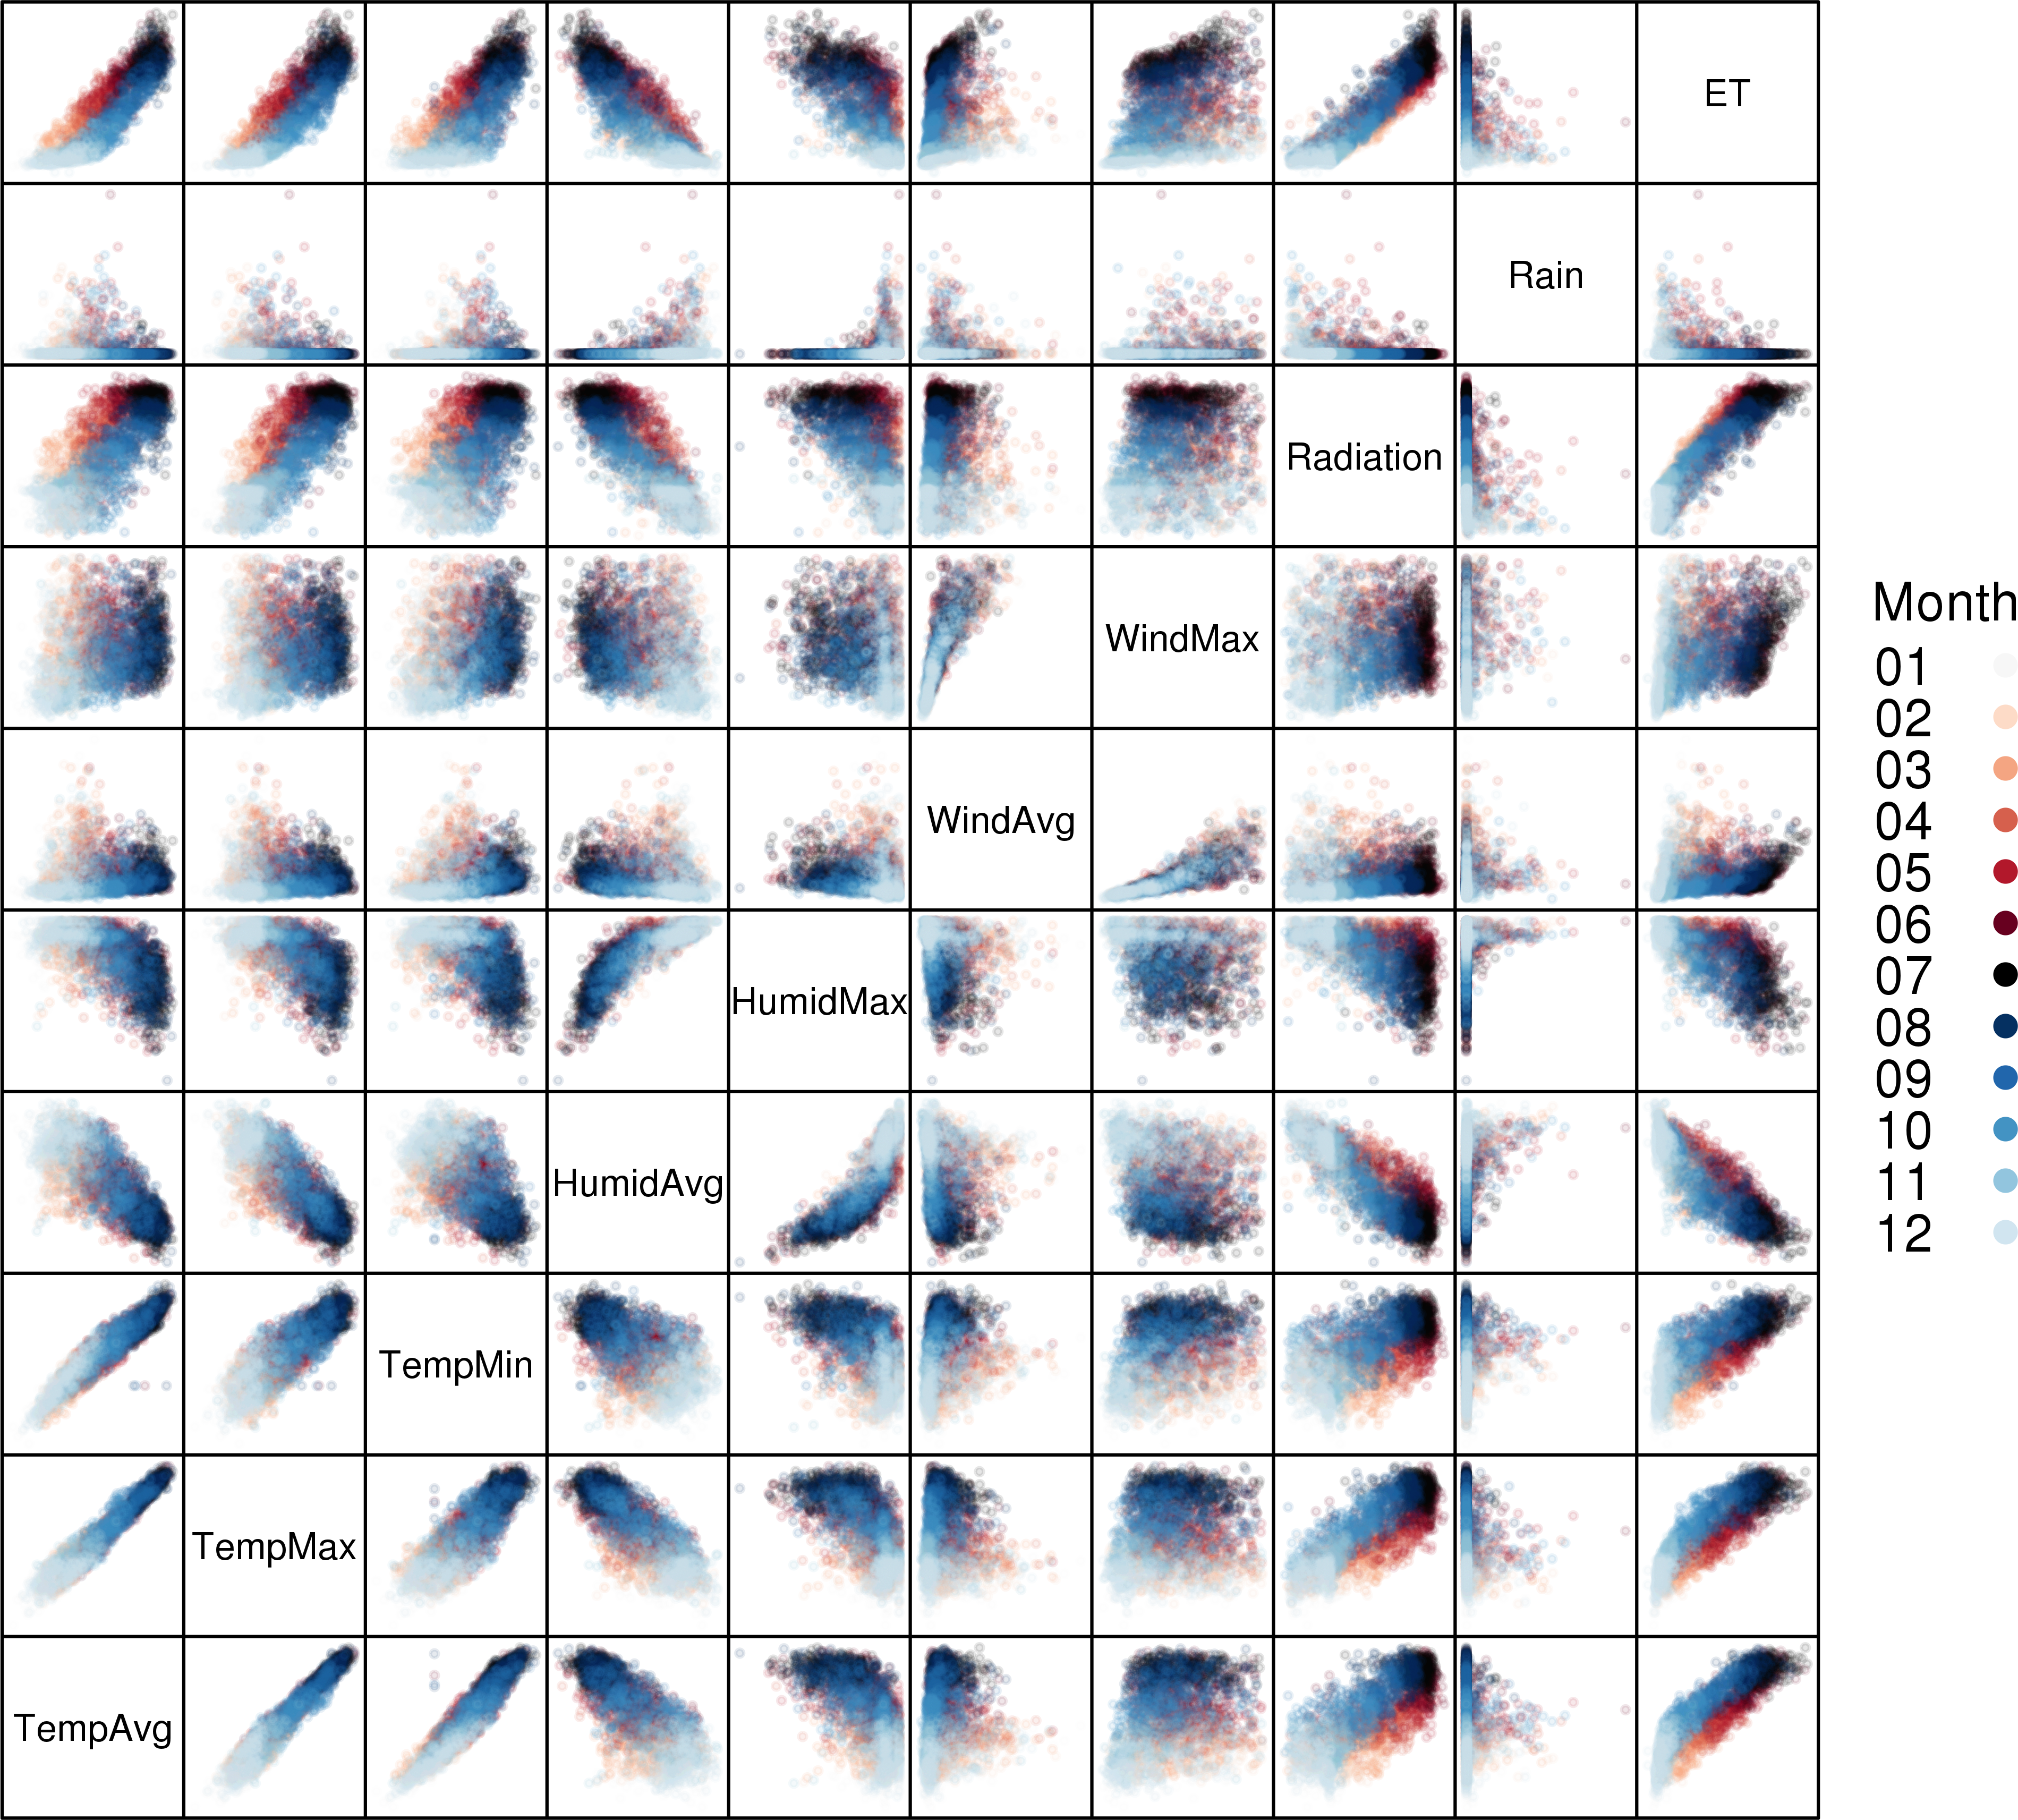
\includegraphics[width=.9\linewidth]{figs/aranjuezSplom.png}
\caption{\label{fig:orgparagraph1}
Scatter plot matrix of the collection of meteorological time series of the Aranjuez station.}
\end{figure}


Let's explore Figure \ref{fig:orgparagraph1}. For example,
\begin{itemize}
\item The highest values of ambient temperature (average, maximum, and
mimimun), solar radiation, and evotranspiration can be found
during the summer.
\item These variables are almost linearly related. The relation
between radiation and temperature is different during both
halves of the year (red and blue regions can be easily distinguished).
\item The humidity reaches its highest values during winter without
appreciable differences between the first and second half of the
year. The temperature and humidity may be related with an
exponential function.
\end{itemize}

A bit of interactivity can be added to this plot with the
identification of some points. This task is easy with
\texttt{panel.link.splom}. The points are selected via mouse clicks (and
highlighted in green). Clicks other than left-clicks terminate the
procedure. The output of this function is the index of chosen
points.

\index{panel.link.splom@\texttt{panel.link.splom}}
\index{trellis.focus@\texttt{trellis.focus}}

\lstset{language=R,label= ,caption= ,captionpos=b,numbers=none}
\begin{lstlisting}
trellis.focus('panel', 1, 1)
idx <- panel.link.splom(pch=13, cex=0.6, col='green')
aranjuez[idx,]
\end{lstlisting}


\subsection{Hexagonal Binning}
\label{sec:orgheadline1}
\label{orgtarget2}

For large datasets, the display of a large number of points in a
scatterplot produces hidden point density, long computation times,
and slow displays. These problems can be circumvented with the
estimation and representation of points densities.  A common
encoding uses gray scales, pseudo colors or partial
transparency. An improved scheme encodes density as the size of
hexagon symbols inscribed within hexagonal binning regions
\cite{Carr.Littlefield.ea1987}.

The \texttt{hexbin} package \cite{Carr.Lewin-Koh.ea2013} includes several
functions for hexagonal binning.  The \texttt{panel.hexbinplot} is a good
substitute for the default panel function. In addition, our first
attempt with \texttt{splom} can be improved with several modifications
(Figure \ref{fig:aranjuezSplomHexbin}):
\begin{itemize}
\item The scale's ticks and labels are suppressed with \texttt{pscale=0}.
\item The panels of the lower part of the matrix (\texttt{lower.panel}) will
include a locally weighted scatterplot smoothing (loess) with
\texttt{panel.loess}.
\item The diagonal panels (\texttt{diag.panel}) will display the kernel
density estimate of each variable. The \texttt{density} function
computes this estimate. The result is adjusted to the panel
limits (calculated with \texttt{current.panel.limits}). The kernel
density is plotted with \texttt{panel.lines} and the \texttt{diag.panel.splom}
function completes the content of each diagonal panel.
\item The point density is encoded with the palette \texttt{BTC} (ligther
colors for high density values and darker colors for almost
empty regions, with a gradient of blue hues for intermediate values).
\end{itemize}

\index{Packages!hexbin@\texttt{hexbin}}
\index{panel.hexbinplot@\texttt{panel.hexbinplot}}
\index{panel.loess@\texttt{panel.loess}}
\index{diag.panel.splom@\texttt{diag.panel.splom}}
\index{current.panel.limits@\texttt{current.panel.limits}}
\index{Panel function}

\lstset{language=R,label= ,caption= ,captionpos=b,numbers=none}
\begin{lstlisting}
  library(hexbin)
  
  splom(~as.data.frame(aranjuez),
             panel=panel.hexbinplot, xlab='',
             colramp=BTC,
             diag.panel = function(x, ...){
               yrng <- current.panel.limits()$ylim
               d <- density(x, na.rm=TRUE)
               d$y <- with(d, yrng[1] + 0.95 * diff(yrng) * y / max(y))
               panel.lines(d)
               diag.panel.splom(x, ...)
             },
             lower.panel = function(x, y, ...){
               panel.hexbinplot(x, y, ...)
               panel.loess(x, y, ..., col = 'red')
             },
             pscale=0, varname.cex=0.7
             )
\end{lstlisting}

\begin{figure}[htb]
\centering
\includegraphics[width=.9\linewidth]{figs/aranjuezSplomHexbin.pdf}
\caption{\label{fig:orgparagraph2}
Scatterplot matrix of the collection of meteorological time series of the Aranjuez station using hexagonal binning.}
\end{figure}

A drawback of the matrix of scatterplots with hexagonal binning is
that each panel is drawn independently, so it is impossible to compute
a common color key for all of them. In other words, two cells with
exactly the same color in different panels encode different point
densities.

It is possible to display a reduced set of variables against
another one and generate a common color key using the \texttt{hexbinplot}
function. First, the dataset must be reshaped from the wide format
(one colum for each variable) to the long format (only one column for
the values with one row for each observation). 

The \texttt{reshape} function needs several arguments to perform the
conversion. The most important is the \texttt{data.frame} to be
transformed. Then there are the names of variables to be mapped to
a single variable in the long dataset (the three ambient
temperatures). The name of this variable can be set with
\texttt{v.names}. Finally, \texttt{timevar} is the name of the column in long format that
differentiates multiple observations from the same variable. The
values of this column are defined with the \texttt{times} argument.

\index{reshape@\texttt{reshape}}

\lstset{language=R,label= ,caption= ,captionpos=b,numbers=none}
\begin{lstlisting}
  aranjuezDF <- data.frame(aranjuez,
                           month=format(index(aranjuez), '%m'))
  aranjuezRshp <- reshape(aranjuezDF, direction='long',
                          varying=list(names(aranjuez)[1:3]),
                          v.names='Temperature',
                          times=names(aranjuez)[1:3],
                          timevar='Statistic')
\end{lstlisting}


\lstset{language=R,label= ,caption= ,captionpos=b,numbers=none}
\begin{lstlisting}
  head(aranjuezRshp)
\end{lstlisting}

The \texttt{hexbinplot} displays this dataset with a different panel for
each type of temperature (average, maximum, and minimum) but with a
common color key encoding the point density (Figure
\ref{fig:orgparagraph3}). Now, two cells with the same color in
different panels encode the same value. 
\index{hexbinplot@\texttt{hexbinplot}}
\index{Panel function}

\lstset{language=R,label= ,caption= ,captionpos=b,numbers=none}
\begin{lstlisting}
  hexbinplot(Radiation~Temperature|Statistic, data=aranjuezRshp,
             layout=c(1, 3), colramp=BTC) +
      layer(panel.loess(..., col = 'red'))
\end{lstlisting}

\begin{figure}[htb]
\centering
\includegraphics[width=.9\linewidth]{figs/aranjuezHexbinplot.pdf}
\caption{\label{fig:orgparagraph3}
Scatterplot with hexagonal binning of temperature versus solar radiation using data of the Aranjuez station (\texttt{lattice} version).}
\end{figure}

The ggplot2 version uses \texttt{stat\_binhex}.
\lstset{language=R,label= ,caption= ,captionpos=b,numbers=none}
\begin{lstlisting}
  ggplot(data=aranjuezRshp, aes(Temperature, Radiation)) +
      stat_binhex(ncol=1) + 
      stat_smooth(se=FALSE, method='loess', col='red') +
      facet_wrap(~Statistic, ncol=1) +
      theme_bw()
\end{lstlisting}

\section{Scatterplot with Time as a Conditioning Variable}
\label{sec:orgheadline3}
\label{orgtarget3}

After discussing the hexagonal binning, let's recover the time
variable. Figure \ref{fig:orgparagraph1} uses colors to encode
months. Instead, we will now display separate scatterplots with a
panel for each month. In addition, the statistic type (average,
maximum, minimum) is included as an additional conditioning variable.

This matrix of panels can be displayed with \texttt{ggplot} using
\texttt{facet\_grid}. The code of Figure \ref{fig:orgparagraph4} uses partial
transparency to cope with overplotting, small horizontal and vertical
segments (\texttt{geom\_rug}) to display points density on both variables, and
a smooth line in each panel.
\lstset{language=R,label= ,caption= ,captionpos=b,numbers=none}
\begin{lstlisting}
  ggplot(data=aranjuezRshp, aes(Radiation, Temperature)) +
      facet_grid(Statistic ~ month) +
      geom_point(col='skyblue4', pch=19, cex=0.5, alpha=0.3) +
      geom_rug() +
      stat_smooth(se=FALSE, method='loess', col='indianred1', lwd=1.2) +
      theme_bw()
\end{lstlisting}

\begin{figure}[htb]
\centering
\includegraphics[width=.9\linewidth]{figs/aranjuezFacetGrid.png}
\caption{\label{fig:orgparagraph4}
Scatterplot of temperature versus solar radiation for each month using data of the Aranjuez station (\texttt{ggplot2} version).}
\end{figure}

The version with \texttt{lattice} needs the \texttt{useOuterStrips} function from
the \texttt{latticeExtra} package, which prints the names of the conditioning
variables on the top and left outer margins (Figure
\ref{fig:orgparagraph5}).

\index{useOuterStrips@\texttt{useOuterStrips}}
\index{panel.rug@\texttt{panel.rug}}
\index{panel.loess@\texttt{panel.loess}}
\index{Packages!latticeExtra@\texttt{latticeExtra}}

\lstset{language=R,label= ,caption= ,captionpos=b,numbers=none}
\begin{lstlisting}
  useOuterStrips(xyplot(Temperature ~ Radiation | month * Statistic,
                        data=aranjuezRshp,
                        between=list(x=0),
                        col='skyblue4', pch=19,
                        cex=0.5, alpha=0.3)) +
      layer({
          panel.rug(..., col.line='indianred1', end=0.05, alpha=0.6)
          panel.loess(..., col='indianred1', lwd=1.5, alpha=1)
      })
\end{lstlisting}

\begin{figure}[htb]
\centering
\includegraphics[width=.9\linewidth]{figs/aranjuezOuterStrips.pdf}
\caption{\label{fig:orgparagraph5}
Scatterplot of temperature versus solar radiation for each month using data of the Aranjuez station (lattice version).}
\end{figure}

These figures show the typical seasonal behavior of solar radiation
and ambient temperature. Additionally, it displays in more detail the
same relations between radiation and temperature already discussed
with Figure \ref{fig:orgparagraph3}.

\chapter{Time as a Complementary Variable}
\label{sec:orgheadline21}
\label{cha:timeComplementary}

Gapminder \footnote{\url{http://www.gapminder.org/}} is an independent foundation based in Stockholm, Sweden.  Its mission is ``to debunk devastating myths about the world by offering free access to a fact-based world view.'' They provide free online tools, data, and videos ``to better understand the changing world.'' The initial development of Gapminder was the Trendalyzer software, used by Hans Rosling in several sequences of his documentary ``The Joy of Stats.''

The information visualization technique used by Trendalyzer is an interactive bubble chart. By default it shows five variables: two numeric variables on the vertical and horizontal axes, bubble size and color, and a time variable that may be manipulated with a slider. The software uses brushing and linking techniques for displaying the numeric value of a highlighted country.

This software was acquired by Google in 2007, and is now available as a Motion Chart gadget and as the Public Data Explorer.

In this chapter, time will be used as a complementary variable which adds information to a graph where several variables are confronted. We will illustrate this approach with the evolution of the relationship between Gross National Income (GNI) and carbon dioxide (\(CO_2\)) emissions for a set of countries extracted from the database of the World Bank Open Data. We will try several solutions to display the relationship between \(CO_2\) emissions and GNI over the years using time as a complementary variable. The final method will produce an animated plot resembling the Trendalyzer solution.

\section{Polylines}
\label{sec-1}
The first solution is a Motion Chart the \texttt{googleVis} package
\cite{Gesmann.deCastillo2011}, an interface between R and the Google
Visualisation API. With its \texttt{gvisMotionChart} function it is easy to
produce a Motion Chart that can be displayed using a browser with
Flash enabled (Figure \ref{fig:googleVis}).

\lstset{language=R,numbers=none}
\begin{lstlisting}
load('data/CO2.RData')
\end{lstlisting}



\index{Data!CO2@$CO_2$}
\index{Data!World Bank}
\index{Packages!googleVis@\texttt{googleVis}}

\lstset{language=R,numbers=none}
\begin{lstlisting}
library(googleVis)
pgvis <- gvisMotionChart(CO2data, idvar='Country.Name', timevar='Year')
\end{lstlisting}

\begin{figure}
  \centering
  \includegraphics[width=\textwidth]{figs/googleVis}
  \caption{Snapshot of a Motion Chart produced with googleVis.}
  \label{fig:googleVis}
\end{figure}



Although the \texttt{gvisMotionChart} is quite easy to use, the global
appearance and behavior are completely determined by Google
API\footnote{You should read the Google API Terms of Service before using
  \texttt{googleVis}: \url{https://developers.google.com/terms/}.}. Moreover, you should carefully read their Terms of Use
before using it for public distribution.

Our next attempt is to display the entire data in a panel with a
scatterplot using country names as the grouping factor. Points of each
country are connected with polylines to reveal the time evolution
(Figure \ref{fig:CO2-GNI}).
\lstset{language=R,numbers=none}
\begin{lstlisting}
## lattice version
xyplot(GNI.capita  ~ CO2.capita, data=CO2data,
       xlab="Carbon dioxide emissions (metric tons per capita)",
       ylab="GNI per capita, PPP (current international $)",
       groups=Country.Name, type='b')
\end{lstlisting}

\begin{figure}[htb]
\centering
\includegraphics[width=.9\linewidth]{figs/CO2_GNI.pdf}
\caption{\label{fig:CO2-GNI}GNI per capita versus $\mathrm{CO_2}$ emissions per capita (\texttt{lattice} version).}
\end{figure}

\lstset{language=R,numbers=none}
\begin{lstlisting}
## ggplot2 version
ggplot(data=CO2data, aes(x=CO2.capita, y=GNI.capita,
           color=Country.Name)) +
    xlab("Carbon dioxide emissions (metric tons per capita)") +
    ylab("GNI per capita, PPP (current international $)") +
    geom_point() + geom_path() + theme_bw()
\end{lstlisting}

Three improvements can be added to this graphical result: 
\begin{enumerate}
\item Define a better palette to enhance visual discrimination between
countries.
\item Display time information with labels to show year values.
\item Label each polyline with the country name instead of a legend.
\end{enumerate}
\section{Choosing Colors}
\label{sec-2}
The \texttt{Country.Name} categorical variable will be encoded with a
qualitative palette, namely the first five colors of \texttt{Set1}
palette\footnote{\url{http://colorbrewer2.org/}} from the \texttt{RColorBrewer} package
\cite{Neuwirth2011}. Because there are more countries than colors, we
have to repeat some colors to complete the number of levels of the
variable \texttt{Country.Name}. The result is a palette with non-unique
colors, and thus some countries will share the same color. This is not
a problem because the curves will be labeled, and countries with the
same color will be displayed at enough distance.

\index{Packages!RColorBrewer@\texttt{RColorBrewer}}
\index{brewer.pal@\texttt{brewer.pal}}

\lstset{language=R,numbers=none}
\begin{lstlisting}
library(RColorBrewer)

nCountries <- nlevels(CO2data$Country.Name)
pal <- brewer.pal(n=5, 'Set1')
pal <- rep(pal, length = nCountries)
\end{lstlisting}

Adjacent colors of this palette are chosen to be easily
distinguishable. Therefore, the connection between colors and
countries must be in such a way that nearby lines are encoded
with adjacent colors of the palette.

A simple approach is to calculate the annual average of the
variable to be represented along the x-axis (\texttt{CO2.capita}), and
extract colors from the palette according to the order of this
value.  

\index{aggregate@\texttt{aggregate}}

\lstset{language=R,numbers=none}
\begin{lstlisting}
## Rank of average values of CO2 per capita
CO2mean <- aggregate(CO2.capita ~ Country.Name, data=CO2data, FUN=mean)
palOrdered <- pal[rank(CO2mean$CO2.capita)]
\end{lstlisting}

A more sophisticated solution is to use the ordered results of a
hierarchical clustering of the time evolution of the $\mathrm{CO_2}$ per capita
values (Figure \ref{fig:hclustCO2}). The data is extracted from the
original $\mathrm{CO_2}$ \texttt{data.frame}.  

\index{hclust@\texttt{hclust}}

\lstset{language=R,numbers=none}
\begin{lstlisting}
CO2capita <- CO2data[, c('Country.Name', 'Year', 'CO2.capita')]
CO2capita <- reshape(CO2capita, idvar='Country.Name', timevar='Year', direction='wide')
hCO2 <- hclust(dist(CO2capita[, -1]))

oldpar <- par(mar=c(0, 2, 0, 0) + .1)
plot(hCO2, labels=CO2capita$Country.Name,
     xlab='', ylab='', sub='', main='')
par(oldpar)
\end{lstlisting}

\begin{figure}[htb]
\centering
\includegraphics[width=.9\linewidth]{figs/hclust.pdf}
\caption{\label{fig:hclustCO2}Hierarchical clustering of the time evolution of $\mathrm{CO_2}$ per capita values.}
\end{figure}


The colors of the palette are assigned to each country with \texttt{match},
which returns a vector of the positions of the matches of the country
names in alphabetical order in the country names ordered according to
the hierarchical clustering.
\lstset{language=R,numbers=none}
\begin{lstlisting}
idx <- match(levels(CO2data$Country.Name), 
             CO2capita$Country.Name[hCO2$order])
palOrdered <- pal[idx]
\end{lstlisting}
It must be highlighted that this palette links colors with the levels
of \texttt{Country.Name} (country names in alphabetical order), which is
exactly what the \texttt{groups} argument provides. The following code
produces a curve for each country using different colors to
distinguish them.

\index{simpleTheme@\texttt{simpleTheme}}

\lstset{language=R,numbers=none}
\begin{lstlisting}
## simpleTheme encapsulates the palette in a new theme for xyplot
myTheme <- simpleTheme(pch=19, cex=0.6, col=palOrdered)

pCO2.capita <- xyplot(GNI.capita  ~ CO2.capita,
                      xlab="Carbon dioxide emissions (metric tons per capita)",
                      ylab="GNI per capita, PPP (current international $)",
                      groups=Country.Name, data=CO2data,
                      par.settings=myTheme,
                      type='b')
\end{lstlisting}

\lstset{language=R,numbers=none}
\begin{lstlisting}
gCO2.capita <- ggplot(data=CO2data, aes(x=CO2.capita, y=GNI.capita,
                      color=Country.Name)) +
    geom_point() + geom_path() +
    scale_color_manual(values=palOrdered, guide=FALSE) +
    xlab('CO2 emissions (metric tons per capita)') +
    ylab('GNI per capita, PPP (current international $)') +
    theme_bw()
\end{lstlisting}
\section{Labels to Show Time Information}
\label{sec-3}
This result can be improved with labels displaying the years to show
the time evolution.  A panel function with \texttt{panel.text} to print the
year labels and \texttt{panel.superpose} to display the lines for each group
is a solution. In the panel function, \texttt{subscripts} is a vector with
the integer indices representing the rows of the \texttt{data.frame} to be
displayed in the panel.

\index{panel.text@\texttt{panel.text}}
\index{subscripts@\texttt{subscripts}} \index{Panel function}
\index{panel.superpose@\texttt{panel.superpose}}

\lstset{language=R,numbers=none}
\begin{lstlisting}
xyplot(GNI.capita  ~ CO2.capita,
       xlab="Carbon dioxide emissions (metric tons per capita)",
       ylab="GNI per capita, PPP (current international $)",
       groups=Country.Name, data=CO2data,
       par.settings=myTheme,
       type='b', 
       panel=function(x, y, ..., subscripts, groups){
         panel.text(x, y, ...,
                    labels=CO2data$Year[subscripts],
                    pos=2, cex=0.5, col='gray')
         panel.superpose(x, y, subscripts, groups,...)
       }
       )
\end{lstlisting}

The same result with a clearer code is obtained with the combination
of \texttt{+.trellis}, \texttt{glayer\_} and \texttt{panel.text}. Using \texttt{glayer\_} instead of
\texttt{glayer}, we ensure that the labels are printed below the lines.

\index{Packages!latticeExtra@\texttt{latticeExtra}}
\index{glayer@\texttt{glayer}}
\index{+.trellis@\texttt{+.trellis}}

\lstset{language=R,numbers=none}
\begin{lstlisting}
pCO2.capita <- pCO2.capita +
    glayer_(panel.text(..., labels=CO2data$Year[subscripts],
                       pos=2, cex=0.5, col='gray'))
\end{lstlisting}

\lstset{language=R,numbers=none}
\begin{lstlisting}
gCO2.capita <- gCO2.capita + geom_text(aes(label=Year),
                                       colour='gray',
                                       size=2.5,
                                       hjust=0, vjust=0)
\end{lstlisting}
\section{Country Names: Positioning Labels}
\label{sec-4}
The common solution to link each curve with the group value is to add
a legend. However, a legend can be confusing with too many items. In
addition, the reader must carry out a complex task: Choose the line,
memorize its color, search for it in the legend, and read the country
name.

A better approach is to label each line using nearby text with the
same color encoding. A suitable method is to place the labels
close to the end of each line (Figure
\ref{fig:CO2-GNI-glayer}). Labels are placed with the
\texttt{panel.pointLabel} function from the \texttt{maptools} package. This
function use optimization routines to find locations without
overlaps.

\index{group.value@\texttt{group.value}}
\index{group.number@\texttt{group.number}}

\lstset{language=R,numbers=none}
\begin{lstlisting}
library(maptools)  
## group.value provides the country name; group.number is the
## index of each country to choose the color from the palette.
pCO2.capita +
    glayer(panel.pointLabel(mean(x), mean(y),
                            labels= group.value,
                            col=palOrdered[group.number],
                            cex=.8,
                            fontface=2, fontfamily='Palatino'))
\end{lstlisting}

\begin{figure}[htb]
\centering
\includegraphics[width=.9\linewidth]{figs/CO2_capita.pdf}
\caption{\label{fig:CO2-GNI-glayer}$\mathrm{CO_2}$ emissions versus GNI per capita. Labels are placed with \texttt{panel.pointLabel}.}
\end{figure}


However, this solution does not solve the overlapping between labels
and lines. The package \texttt{directlabels} \cite{Hocking2013} includes a
wide repertory of positioning methods to cope with this problem. The
main function, \texttt{direct.label}, is able to determine a suitable method
for each plot, although the user can choose a different method from
the collection or even define a custom method. For the \texttt{pCO2.capita}
object, I have obtained the best results with \texttt{extreme.grid} (Figure
\ref{fig:CO2-GNI-DL}).

\index{Packages!directlabels@\texttt{directlabels}}
\index{direct.label@\texttt{direct.label}}

\lstset{language=R,numbers=none}
\begin{lstlisting}
library(directlabels)
direct.label(pCO2.capita, method='extreme.grid')
\end{lstlisting}

\begin{figure}[htb]
\centering
\includegraphics[width=.9\linewidth]{figs/CO2_capitaDL.pdf}
\caption{\label{fig:CO2-GNI-DL}$\mathrm{CO_2}$ emissions versus GNI per capita. Labels are placed with the \texttt{extreme.grid} method of the \texttt{directlabels} package.}
\end{figure}

\lstset{language=R,numbers=none}
\begin{lstlisting}
direct.label(gCO2.capita, method='extreme.grid')
\end{lstlisting}
\section{A Panel for Each Year}
\label{sec-5}
Time can be used as a conditioning variable (as shown in previous
sections) to display subsets of the data in different panels. Figure
\ref{fig:CO2-GNI-panel} is produced with the same code as in Figure
\ref{fig:CO2-GNI}, now including \texttt{|factor(Year)} in the lattice
version and \texttt{facet\_wrap(\textasciitilde{} Year)} in the \texttt{ggplot2} version.

\lstset{language=R,numbers=none}
\begin{lstlisting}
xyplot(GNI.capita  ~ CO2.capita | factor(Year), data=CO2data,
       xlab="Carbon dioxide emissions (metric tons per capita)",
       ylab="GNI per capita, PPP (current international $)",
       groups=Country.Name, type='b',
       auto.key=list(space='right'))
\end{lstlisting}

\begin{figure}[htb]
\centering
\includegraphics[width=.9\linewidth]{figs/CO2_capita_panel.pdf}
\caption{\label{fig:CO2-GNI-panel}$\mathrm{CO_2}$ emissions versus GNI per capita with a panel for each year.}
\end{figure}

\lstset{language=R,numbers=none}
\begin{lstlisting}
ggplot(data=CO2data, aes(x=CO2.capita, y=GNI.capita, colour=Country.Name)) +
    facet_wrap(~ Year) + geom_point(pch=19) + 
    xlab('CO2 emissions (metric tons per capita)') +
    ylab('GNI per capita, PPP (current international $)') +
    theme_bw()
\end{lstlisting}

Because the grouping variable, \texttt{Country.Name}, has many levels, the
legend is not very useful. Once again, point labeling is recommended
(Figure \ref{fig:CO2-GNI-panel-labels}).

\lstset{language=R,numbers=none}
\begin{lstlisting}
xyplot(GNI.capita  ~ CO2.capita | factor(Year), data=CO2data,
       xlab="Carbon dioxide emissions (metric tons per capita)",
       ylab="GNI per capita, PPP (current international $)",
       groups=Country.Name, type='b',
       par.settings=myTheme) + 
    glayer(panel.pointLabel(x, y, labels=group.value,
                            col=palOrdered[group.number], cex=0.7))
\end{lstlisting}

\begin{figure}[htb]
\centering
\includegraphics[width=.9\linewidth]{figs/CO2_capita_panel_labels.pdf}
\caption{\label{fig:CO2-GNI-panel-labels}$\mathrm{CO_2}$ emissions versus GNI per capita with a panel for each year.}
\end{figure}

\subsection{\floweroneleft Using Variable Size to Encode an Additional Variable}
\label{sec-5-1}
Instead of using simple points, we can display circles of
different radius to encode a new variable. This new variable is
\texttt{CO2.PPP}, the ratio of $\mathrm{CO_2}$ emissions to the Gross Domestic
Product with purchasing power parity (PPP) estimations.

To use this numeric variable as an additional grouping factor, its
range must be divided into different classes. The typical solution is
to use \texttt{cut} to coerce the numeric variable into a \texttt{factor} whose
levels correspond to uniform intervals, which could be unrelated to
the data distribution. The \texttt{classInt} package \cite{Bivand2013}
provides several methods to partition data into classes based on
natural groups in the data distribution.

\index{Packages!classInt@\texttt{classInt}}
\index{classIntervals@\texttt{classIntervals}}

\lstset{language=R,numbers=none}
\begin{lstlisting}
library(classInt)
z <- CO2data$CO2.PPP
intervals <- classIntervals(z, n=4, style='fisher')
\end{lstlisting}

Although the functions of this package are mainly intended to create
color palettes for maps, the results can also be associated to
point sizes. \texttt{cex.key} defines the sequence of sizes (to be
displayed in the legend) associated with each \texttt{CO2.PPP} using the
\texttt{findCols} function.
\lstset{language=R,numbers=none}
\begin{lstlisting}
nInt <- length(intervals$brks) - 1
cex.key <- seq(0.5, 1.8, length=nInt)

idx <- findCols(intervals)
CO2data$cexPoints <- cex.key[idx]
\end{lstlisting}

The graphic will display information on two variables (\texttt{GNI.capita}
and \texttt{CO2.capita} in the vertical and horizontal axes, respectively)
with a conditioning variable (\texttt{Year}) and two grouping variables
(\texttt{Country.Name}, and \texttt{CO2.PPP} through \texttt{cexPoints}) (Figure
\ref{fig:CO2pointsGG}).

\lstset{language=R,numbers=none}
\begin{lstlisting}
ggplot(data=CO2data, aes(x=CO2.capita, y=GNI.capita, colour=Country.Name)) +
    facet_wrap(~ Year) + geom_point(aes(size=cexPoints), pch=19) +
    xlab('Carbon dioxide emissions (metric tons per capita)') +
    ylab('GNI per capita, PPP (current international $)') +
    theme_bw()
\end{lstlisting}

\begin{figure}[htb]
\centering
\includegraphics[width=.9\linewidth]{figs/CO2pointsGG.pdf}
\caption{\label{fig:CO2pointsGG}$\mathrm{CO_2}$ emissions versus GNI per capita for different intervals of the ratio of $\mathrm{CO_2}$ emissions to the GDP PPP estimations.}
\end{figure}

The \texttt{auto.key} mechanism of the \texttt{lattice} version is not able to cope
with two grouping variables. Therefore, the legend, whose main
componens are the labels (\texttt{intervals}) and the point sizes
(\texttt{cex.key}), should be defined manually (Figure \ref{fig:CO2points}).

\index{panel.text@\texttt{panel.text}}

\lstset{language=R,numbers=none}
\begin{lstlisting}
op <- options(digits=2)
tab <- print(intervals)
options(op)

key <- list(space='right',
            title=expression(CO[2]/GNI.PPP),
            cex.title=1,
            ## Labels of the key are the intervals strings
            text=list(labels=names(tab), cex=0.85),
            ## Points sizes are defined with cex.key
            points=list(col='black', pch=19,
              cex=cex.key, alpha=0.7))


xyplot(GNI.capita ~ CO2.capita|factor(Year), data=CO2data,
       xlab="Carbon dioxide emissions (metric tons per capita)",
       ylab="GNI per capita, PPP (current international $)",
       groups=Country.Name, key=key, alpha=0.7,
       col=palOrdered, cex=CO2data$cexPoints) +
    glayer(panel.pointLabel(x, y, labels=group.value,
                            col=palOrdered[group.number], cex=0.7))
\end{lstlisting}

\begin{figure}[htb]
\centering
\includegraphics[width=.9\linewidth]{figs/CO2points.pdf}
\caption{\label{fig:CO2points}$\mathrm{CO_2}$ emissions versus GNI per capita for different intervals of the ratio of $\mathrm{CO_2}$ emissions to the GDP PPP estimations.}
\end{figure}
\section{\floweroneleft Traveling Bubbles}
\label{sec-6}
The final solution to display this multivariate time series is with
animation via the function \texttt{grid.animate} of the \texttt{gridSVG}
package. We will mimic the Trendalyzer/Motion Chart solution, using
traveling bubbles of different colors and with radius proportional to
\texttt{CO2.PPP}.

The first step is to draw the initial state of the bubbles. Their
colors are again defined by the \texttt{palOrdered} palette, although the
\texttt{adjustcolor} function is used for a ligther \texttt{fill} color. Because
there will not be a legend, there is no need to define class
intervals, and thus the radius is directly proportional to the value
of \texttt{CO2data\$CO2.PPP}.

\index{Packages!gridSVG@\texttt{gridSVG}}

\lstset{language=R,numbers=none}
\begin{lstlisting}
library(gridSVG)

xyplot(GNI.capita ~ CO2.capita, data=CO2data,
       xlab="Carbon dioxide emissions (metric tons per capita)",
       ylab="GNI per capita, PPP (current international $)",
       subset=Year==2000, groups=Country.Name,
       ## The limits of the graphic are defined
       ## with the entire dataset
       xlim=extendrange(CO2data$CO2.capita),
       ylim=extendrange(CO2data$GNI.capita),
       panel=function(x, y, ..., subscripts, groups) {
         color <- palOrdered[groups[subscripts]]
         radius <- CO2data$CO2.PPP[subscripts]
         ## Size of labels
         cex <- 1.1*sqrt(radius)
         ## Bubbles
         grid.circle(x, y, default.units="native",
                     r=radius*unit(.25, "inch"),
                     name=trellis.grobname("points", type="panel"),
                     gp=gpar(col=color,
                       ## Fill color ligther than border
                       fill=adjustcolor(color, alpha=.5),
                       lwd=2))
         ## Country labels
         grid.text(label=groups[subscripts],
                   x=unit(x, 'native'),
                   ## Labels above each bubble
                   y=unit(y, 'native') + 1.5 * radius *unit(.25, 'inch'),
                   name=trellis.grobname('labels', type='panel'),
                   gp=gpar(col=color, cex=cex))
       })
\end{lstlisting}

From this initial state, \texttt{grid.animate} creates a collection of
animated graphical objects with the result of \texttt{animUnit}. This
function produces a set of values that will be interpreted by
\texttt{grid.animate} as intermediate states of a feature of the graphical
object. Thus, the bubbles will travel across the values defined by
\texttt{x\_points} and \texttt{y\_points}, while their labels will use \texttt{x\_points} and
\texttt{x\_labels}.

The use of \texttt{rep=TRUE} ensures that the animation will be repeated
indefinitely.

\index{animUnit@\texttt{animUnit}}
\index{grid.animate@\texttt{grid.animate}}

\lstset{language=R,numbers=none}
\begin{lstlisting}
## Duration in seconds of the animation
duration <- 20

nCountries <- nlevels(CO2data$Country.Name)
years <- unique(CO2data$Year)
nYears <- length(years)

## Intermediate positions of the bubbles
x_points <- animUnit(unit(CO2data$CO2.capita, 'native'),
                     id=rep(seq_len(nCountries), each=nYears))
y_points <- animUnit(unit(CO2data$GNI.capita, 'native'),
                     id=rep(seq_len(nCountries), each=nYears))
## Intermediate positions of the labels
y_labels <- animUnit(unit(CO2data$GNI.capita, 'native') +
                     1.5 * CO2data$CO2.PPP * unit(.25, 'inch'),
                     id=rep(seq_len(nCountries), each=nYears))
## Intermediate sizes of the bubbles
size <- animUnit(CO2data$CO2.PPP * unit(.25, 'inch'),
                     id=rep(seq_len(nCountries), each=nYears))

grid.animate(trellis.grobname("points", type="panel", row=1, col=1),
             duration=duration,
             x=x_points,
             y=y_points,
             r=size,
             rep=TRUE)

grid.animate(trellis.grobname("labels", type="panel", row=1, col=1),
             duration=duration,
             x=x_points,
             y=y_labels,
             rep=TRUE)
\end{lstlisting}

A bit of interactivity can be added with the \texttt{grid.hyperlink}
function. For example, the following code adds the corresponding
Wikipedia link to a mouse click on each bubble.

\index{grid.hyperlink@\texttt{grid.hyperlink}}

\lstset{language=R,numbers=none}
\begin{lstlisting}
countries <- unique(CO2data$Country.Name)
URL <- paste('http://en.wikipedia.org/wiki/', countries, sep='')
grid.hyperlink(trellis.grobname('points', type='panel', row=1, col=1),
               URL, group=FALSE)
\end{lstlisting}

Finally, the time information: The year is printed in the lower
right corner, using the \texttt{visibility} attribute of an animated
\texttt{textGrob} object to show and hide the values.
\lstset{language=R,numbers=none}
\begin{lstlisting}
visibility <- matrix("hidden", nrow=nYears, ncol=nYears)
diag(visibility) <- "visible"
yearText <- animateGrob(garnishGrob(textGrob(years, .9, .15,
                                             name="year",
                                             gp=gpar(cex=2, col="grey")),
                                    visibility="hidden"),
                        duration=20,
                        visibility=visibility,
                        rep=TRUE)
grid.draw(yearText)
\end{lstlisting}

The SVG file produced with \texttt{grid.export} is available at the website
of the book (Figure \ref{fig:bubblesSVG}). Because this animation does
not trace the paths, Figure \ref{fig:CO2-GNI-DL} provides this
information as a static complement.

\index{grid.export@\texttt{grid.export}}

\lstset{language=R,numbers=none}
\begin{lstlisting}
grid.export("figs/bubbles.svg")
\end{lstlisting}

\begin{figure}
  \centering
  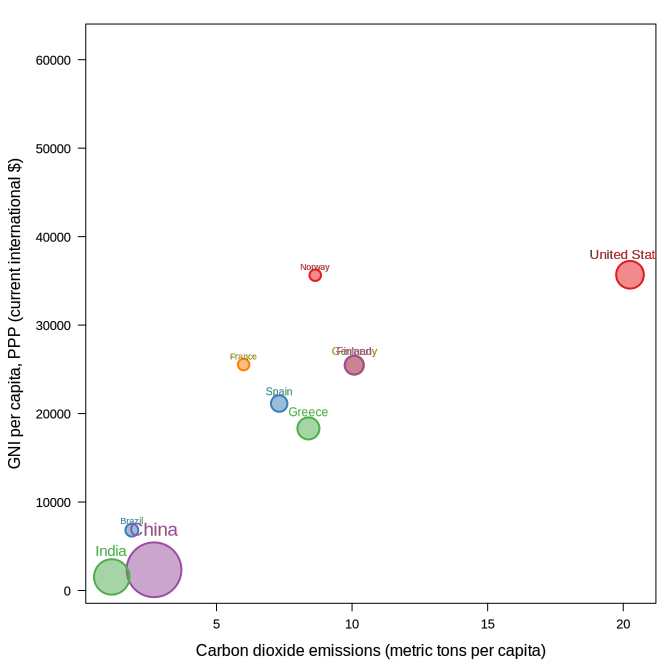
\includegraphics[width=\textwidth]{figs/bubbles.png}
  \caption{Animated bubbles produced with \texttt{gridSVG}.}
  \label{fig:bubblesSVG}
\end{figure}

Now, sit down in your favorite easy chair and watch the magistral
video ``200 Countries, 200 Years, 4 Minutes"\footnote{\url{http://www.gapminder.org/videos/200-years-that-changed-the-world-bbc/}}. After that, you are
ready to open the SVG file of traveling bubbles: It is easier, a short
time period with less than twenty countries.

\chapter{About the Data}
\label{sec:orgheadline22}
\label{cha:dataTime}

\part{Spatial Data}
\label{sec:orgheadline37}

\chapter{Displaying Spatial Data: Introduction}
\label{sec:orgheadline33}
\label{cha:spatialIntro}

Spatial data (also known as geospatial data) are directly or indirectly referenced to a location on the surface of the Earth. Their spatial reference is composed of coordinate values and a system of reference for these coordinates. Spatial data are often accessed, manipulated, or analyzed through Geographic Information Systems (GIS).

Real objects represented by GIS data can be divided into two abstractions: discrete objects (e.g., a road or a river) represented with vector data (points, lines, and polygons), and continuous fields (such as elevation or solar radiation) represented with raster data. The \texttt{sp} package is the preferred option to use vector data in \texttt{R}, and the \texttt{raster} package is the choice for raster data \footnote{Although \texttt{sp} and \texttt{raster} are the most important packages, there are an increasing number of packages designed to work with spatial data. They are summarized in the corresponding CRAN Task View. Read Section \ref{cha:further-reading-spatial} for details.}.

This part exposes several examples where vector and raster data are displayed to show geographic location of features and physical landscape features of a place (reference and physical maps, Chapter \ref{cha:refer-phys-maps}) or a specific variable in the context of a geographic reference (thematic maps, Chapter \ref{cha:thematicMaps}). These examples make use of several datasets (available at the book website) described in Chapter \ref{cha:dataSpatial}.

\section{Packages}
\label{sec:orgheadline31}
\label{sec:spatial-packages}

The CRAN Tasks View ``Analysis of Spatial Data'' \footnote{\url{http://CRAN.R-project.org/view=Spatial}} summarizes the packages for reading, vizualizing, and analyzing spatial data. This section provides a brief introduction to \texttt{sp}, \texttt{raster}, \texttt{rasterVis}, \texttt{maptools}, \texttt{rgdal}, \texttt{gstat}, and \texttt{maps}. Most of the information has been extracted from their vignettes, webpages, and help pages. You should read them for detailed information.

\subsection{sp}
\label{sec:orgheadline24}
\label{sec:sp}

\index{Packages!sp@\texttt{sp}}

The \texttt{sp} package \cite{Pebesma.Bivand2005} provides classes and methods for dealing with spatial data in \texttt{R}. The spatial data classes implemented are points (\texttt{SpatialPoints}), grids (\texttt{SpatialPixels} and \texttt{SpatialGrid}), lines (\texttt{Line}, \texttt{Lines} and \texttt{SpatialLines}), rings, and polygons (\texttt{Polygon}, \texttt{Polygons}, and \texttt{SpatialPolygons}), each of them without data or with data (for example, \texttt{SpatialPointsDataFrame} or \texttt{SpatialLinesDataFrame}).

Selecting, retrieving, or replacing certain attributes in spatial objects with data is done using standard methods:

\begin{itemize}
\item \texttt{[} selects rows (items) and columns in the \texttt{data.frame}.

\item \texttt{[[} selects a column from the \texttt{data.frame}

\item \texttt{[[<-} assigns or replaces values to a column in the \texttt{data.frame}.
\end{itemize}

A number of spatial methods are available for the classes in \texttt{sp}:

\begin{itemize}
\item \texttt{coordinates(object) <- value} sets spatial coordinates to create spatial data. It promotes a \texttt{data.frame} into a \texttt{SpatialPointsDataFrame}. \emph{value} may be specified by a formula, a character vector, or a numeric matrix or \texttt{data.frame} with the actual coordinates.

\item \texttt{coordinates(object, ...)} returns a matrix with the spatial coordinates. If used with \texttt{SpatialPolygons} it returns a matrix with the centroids of the polygons.

\item \texttt{bbox} returns a matrix with the coordinates bounding box.

\item \texttt{proj4string(object)} and \texttt{proj4string(object) <- value} retrieve or set projection attributes on spatial classes.

\item \texttt{spTransform} transforms from one coordinate reference system (geographic projection) to another (requires package \texttt{rgdal}).

\item \texttt{spplot} plots attributes combined with spatial data: Points, lines, grids, polygons.
\end{itemize}

\subsection{raster}
\label{sec:orgheadline25}
\label{sec:raster}

\index{Packages!raster@\texttt{raster}}

The \texttt{raster} package \cite{Hijmans2013} has functions for creating, reading, manipulating, and writing raster data. The package provides general raster data manipulation functions. The package also implements raster algebra and most functions for raster data manipulation that are common in Geographic Information Systems (GIS).

The raster package can work with raster datasets stored on disk if they are too large to be loaded into memory. The package can work with large files because the objects it creates from these files only contain information about the structure of the data, such as the number of rows and columns, the spatial extent, and the filename, but it does not attempt to read all the cell values in memory. In computations with these objects, the data are processed in chunks.

The package defines a number of \texttt{S4} classes. \texttt{RasterLayer}, \texttt{RasterBrick}, and \texttt{RasterStack} are the most important:

\begin{itemize}
\item A \texttt{RasterLayer} object represents single-layer (variable) raster
data. It can be created with the function \texttt{raster}. This function is able to create a \texttt{RasterLayer} from another object, including another \texttt{Raster*} object, or from a \texttt{SpatialPixels*} and \texttt{SpatialGrid*} object, or even a matrix. In addition, it can create a \texttt{RasterLayer} reading data from a file. The \texttt{raster} package can use raster files in several formats, some of them via the \texttt{rgdal} package. Supported formats for reading include GeoTIFF, ESRI, ENVI, and ERDAS.

\item \texttt{RasterBrick} and \texttt{RasterStack} are classes for multilayer data. A
\texttt{RasterStack} is a list of \texttt{RasterLayer} objects with the same spatial extent and resolution. It can be formed with a collection of files in different locations or even mixed with \texttt{RasterLayer} objects that only exist in memory. A \texttt{RasterBrick} is truly a multilayered object, and processing it can be more efficient than processing a \texttt{RasterStack} representing the same data.
\end{itemize}

The \texttt{raster} package defines a number of methods for raster algebra with \texttt{Raster*} objects: arithmetic operators, logical operators, and functions such as \texttt{abs}, \texttt{round}, \texttt{ceiling}, \texttt{floor}, \texttt{trunc}, \texttt{sqrt}, \texttt{log}, \texttt{log10}, \texttt{exp}, \texttt{cos}, \texttt{sin}, \texttt{max}, \texttt{min}, \texttt{range}, \texttt{prod}, \texttt{sum}, \texttt{any}, and \texttt{all}. In these functions, \texttt{Raster*} objects can be mixed with numbers.

There are several functions to modify the content or the spatial extent of \texttt{Raster*} objects, or to combine \texttt{Raster*} objects:

\begin{itemize}
\item The \texttt{crop} function takes a geographic subset of a larger \texttt{Raster*} object. \texttt{trim} crops a \texttt{RasterLayer} by removing the outer rows and columns that only contain \texttt{NA} values. \texttt{extend} adds new rows and/or columns with \texttt{NA} values.

\item The \texttt{merge} function merges two or more \texttt{Raster*} objects into a single new object.

\item \texttt{projectRaster} transforms values of a \texttt{Raster*} object to a new object with a different coordinate reference system.

\item With \texttt{overlay}, multiple \texttt{Raster*} objects can be combined (for example, multiply them).

\item \texttt{mask} removes all values from one layer that are \texttt{NA} in another layer, and \texttt{cover} combines two layers by taking the values of the first layer except where these are \texttt{NA}.

\item \texttt{calc} computes a function for a \texttt{Raster*} object. With \texttt{RasterLayer} objects, another \texttt{RasterLayer} is returned. With multilayer objects the result depends on the function: With a summary function (\texttt{sum}, \texttt{max}, etc.), \texttt{calc} returns a \texttt{RasterLayer} object, and a \texttt{RasterBrick} object otherwise.

\item \texttt{stackApply} computes summary layers for subsets of a \texttt{RasterStack} or \texttt{RasterBrick}.

\item \texttt{cut} and \texttt{reclassify} replace ranges of values with single values.

\item \texttt{zonal} computes zonal statistics, that is, summarizes a \texttt{Raster*} object using zones (areas with the same integer number) defined by another \texttt{RasterLayer}.
\end{itemize}

\subsection{rasterVis}
\label{sec:orgheadline26}
\label{sec:rasterVis}
\index{Packages!rasterVis@\texttt{rasterVis}}

The \texttt{rasterVis} package \cite{Perpinan.Hijmans2013} complements the \texttt{raster} package, providing a set of methods for enhanced visualization and interaction. This package defines visualization methods (\texttt{levelplot}) for quantitative data and categorical data, both for univariate and multivariate rasters.

It also includes several methods in the frame of the Exploratory Data Analysis approach: scatterplots with \texttt{xyplot}, histograms and density plots with \texttt{histogram} and \texttt{densityplot}, violin and boxplots with \texttt{bwplot}, and a matrix of scatterplots with \texttt{splom}.

On the other hand, this package is able to display vector fields using arrows, \texttt{vectorplot}, or with streamlines \cite{Wegenkittl.Groeller1997}, \texttt{streamplot}. In this last method, for each point, \emph{droplet}, of a jittered regular grid, a short streamline portion, \emph{streamlet}, is calculated by integrating the underlying vector field at that point. The main color of each streamlet indicates local vector magnitude (slope). Streamlets are composed of points whose sizes, positions, and color degradation encode the local vector direction (aspect).

\subsection{maptools}
\label{sec:orgheadline27}
\label{sec:maptools}
\index{Packages!maptools@\texttt{maptools}}

The \texttt{maptools} package \cite{Bivand.Lewin-Koh2013} provides a set of tools for manipulating and reading geographic data, in particular ESRI (Environmental Systems Research Institute) shapefiles. The package also provides interface wrappers for exchanging spatial objects with packages such as PBSmapping, spatstat, maps, RArcInfo, Stata tmap, WinBUGS, Mondrian, and others. The main functions in the context of this book are

\begin{itemize}
\item \texttt{readShapePoints} reads data from a points shapefile into a \texttt{SpatialPointsDataFrame} object.

\item \texttt{writePointsShape} writes data from a \texttt{SpatialPointsDataFrame} object to a shapefile.

\item \texttt{readShapeLines} reads data from a line shapefile into a \texttt{SpatialLinesDataFrame} object.

\item \texttt{writeLinesShape} writes data from a \texttt{SpatialLinesDataFrame} object to a shapefile.

\item \texttt{readShapePoly} reads data from a polygon shapefile into a \texttt{SpatialPolygonsDataFrame} object.

\item \texttt{writePolyShape} writes data from a \texttt{SpatialPolygonsDataFrame} object to a shapefile.

\item \texttt{map2SpatialPolygons} and \texttt{map2SpatialLines} may be used to convert map objects returned by the \texttt{map} function in the \texttt{maps} package to the classes defined in the \texttt{sp} package.

\item \texttt{spCbind} provides cbind-like methods for \texttt{Spatial*DataFrame} and \texttt{data.frame} objects.
\end{itemize}

The topology operations on geometries performed by this package (for example, \texttt{unionSpatialPolygons} ) use the package \texttt{rgeos}, an interface to the Geometry Engine Open Source (GEOS) \footnote{\url{http://trac.osgeo.org/geos/}}.

\subsection{rgdal}
\label{sec:orgheadline28}
\label{sec:rgdal}
\index{Packages!rgdal@\texttt{rgdal}}

The \texttt{rgdal} package \cite{Bivand.Keitt.ea2013} provides bindings to the Geospatial Data Abstraction Library (GDAL) \footnote{\url{http://www.gdal.org/}}. With \texttt{readOGR} and \texttt{readGDAL}, both GDAL raster and OGR vector map data can be imported into \texttt{R}, and GDAL raster data and OGR vector data can be exported with \texttt{writeGDAL} and \texttt{writeOGR}.

In addition, this package provides access to projection and transformation operations from the PROJ.4 library \footnote{\url{https://trac.osgeo.org/proj/}}. This package implements several \texttt{spTransform} methods providing transformation between datums and conversion between projections using PROJ.4 projection arguments.

\subsection{gstat}
\label{sec:orgheadline29}
\label{sec:gstat}
\index{Packages!gstat@\texttt{gstat}}

The \texttt{gstat} package \cite{Pebesma2004} provides functions for geostatistical modeling, prediction, and simulation, including variogram modeling and simple, ordinary, universal, and external drift kriging.

Most of the functionality of this package is beyond the scope of this book. However, some functions must be mentioned:

\begin{itemize}
\item \texttt{variogram} calculates the sample variogram from data, or for the residuals if a linear model is given. \texttt{vgm} generates a variogram and \texttt{fit.variogram} fit ranges and/or sills from a variogram model to a sample variogram.

\item \texttt{krige} is the function for simple, ordinary or universal kriging.  \texttt{gstat} is the function for univariate or multivariate geostatistical prediction.
\end{itemize}

\subsection{maps}
\label{sec:orgheadline30}
\label{sec:maps}
\index{Packages!maps@\texttt{maps}}
\index{Packages!mapproj@\texttt{mapproj}}
\index{Packages!mapdata@\texttt{mapdata}}

The \texttt{maps} \cite{Becker.Wilks.ea2013}, \texttt{mapdata} \cite{Becker.Wilks.ea2013b}, and \texttt{mapproj} \cite{McIlroy.Brownrigg.ea2013} packages are useful to draw or create geographical maps. \texttt{mapdata} contains higher resolution databases, and \texttt{mapproj} converts latitude/longitude coordinates into projected coordinates.

\section{Further Reading}
\label{sec:orgheadline32}
\label{cha:further-reading-spatial}

\begin{itemize}
\item \cite{Slocum.McMaster.ea2005} and \cite{Dent.Torguson.ea2008} are comprehensive books on thematic cartography and geovisualization.  They include chapters devoted to data classification, scales, map projections, color theory, typography, and proportional symbol, choropleth, dasymetric, isarithmic, and multivariate mapping. Several resources are available at their accompanying websites \footnote{\url{http://www.pearsonhighered.com/slocum3e/} and
\url{http://highered.mcgraw-hill.com/sites/0072943823/}}.

\item \cite{Bivand.Pebesma.ea2008} is the essential reference to work with spatial data in \texttt{R}. R. Bivand and E. Pebesma are the authors of the fundamental \texttt{sp} package, and they are the authors or maintainers of several important packages such as \texttt{gstat}, for geostatistical modeling, prediction, and simulation, \texttt{rgdal}, \texttt{rgeos} and \texttt{maptools}. Chapter 3 is devoted to the visualization of spatial data. Code, figures, and data of the book are available at the accompanying website \footnote{\url{http://www.asdar-book.org/}}.

\item \cite{Hengl2009} is an open-access book with seven spatial data analysis exercises. The author is the creator and maintainer of the Spatial-Analyst webpage \footnote{\url{http://spatial-analyst.net}}.

\item The CRAN Tasks View ``Analysis of Spatial Data'' \footnote{\url{http://CRAN.R-project.org/view=Spatial}} summarizes the packages for reading, vizualizing, and analyzing spatial data. The packages in development published at R-Forge are listed in the ``Spatial Data \& Statistics'' topic view \footnote{\url{http://r-forge.r-project.org/softwaremap/trove_list.php?form_cat=353}}. The R-SIG-Geo mailing list \footnote{\url{https://stat.ethz.ch/mailman/listinfo/R-SIG-Geo/}} is a powerful resource for obtaining help.

\item The ``Spatial Analysis'' \footnote{\url{http://spatialanalysis.co.uk/map-gallery/}} and ``Kartograph'' \footnote{\url{http://kartograph.org/}} webpages publish a variety of beautiful visualization examples.
\end{itemize}

\chapter{Thematic Maps}
\label{sec:orgheadline34}
\label{cha:thematicMaps}

A thematic map focuses on a specific theme or variable, commonly using geographic data such as coastlines, boundaries, and places as points of reference for the variable being mapped. These maps provide specific information about particular locations or areas (proportional symbol mapping and choropleth maps) and information about spatial patterns (isarithmic and raster maps). The following sections illustrate the code you need to produce these maps, with a final section devoted to the visualization of vector fields.
\section{Proportional Symbol Mapping}
\label{sec-1}
\label{sec:bubble}
\subsection{Introduction}
\label{sec-1-1}
The proportional symbol technique uses symbols of different sizes
to represent data associated with areas or point locations, with
circles being the most frequently used geometric symbol. The data
and the size of symbols can be related through different types of
scaling: mathematical scaling sizes areas of point symbols in
direct proportion to the data; perceptual scaling corrects the
mathematical scaling to account for visual understimation of
larger symbols; and range grading, where data are grouped, and each
class is represented with a single symbol size. 

In this chapter we display data from a grid of sensors belonging to
the Integrated Air Quality system of the Madrid City Council (Section
\ref{sec:airQualityData}) with circles as the proportional symbol, and
range grading as the scaling method. The objective when using range
grading is to discriminate between classes instead of estimating an
exact value from a perceived symbol size. However, because human
perception of symbol size is limited, it is always recommended to
add a second perception channel to improve the discrimination
task. Colors from a sequential palette will complement symbol size to
encode the groups.

\subsection{Proportional Symbol with \texttt{spplot}}
\label{sec-1-2}
The \texttt{NO2sp} \texttt{SpatialPointsDataFrame} can be easily displayed
with the \texttt{spplot} method provided by the \texttt{sp} package, based on
\texttt{xyplot} from the \texttt{lattice} package. Both color and size can be
combined in a unique graphical output because \texttt{spplot} accepts
both of them (Figure \ref{fig:airMadrid_spplot}). I define a
sequential palette whose colors denote the value of the variable
(green for lower values of the contaminant, brown for intermediate
values, and black for highest values).

\lstset{language=R,numbers=none}
\begin{lstlisting}
library(sp)

load('data/NO2sp.RData')
\end{lstlisting}

\lstset{language=R,numbers=none}
\begin{lstlisting}
airPal <- colorRampPalette(c('springgreen1', 'sienna3', 'gray5'))(5)

spplot(NO2sp["mean"], col.regions=airPal, cex=sqrt(1:5),
       edge.col='black', scales=list(draw=TRUE),
       key.space='right')
\end{lstlisting}

\begin{figure}[htb]
\centering
\includegraphics[width=.9\linewidth]{figs/airMadrid_spplot.pdf}
\caption{\label{fig:airMadrid_spplot}Annual average of $NO_2$ measurements in Madrid. Values are shown with different symbol sizes and  colors for each class with the \texttt{spplot} function.}
\end{figure}

The \texttt{ggplot2} version of this code needs to transform the
\texttt{SpatialPointsDataFrame} to a conventional \texttt{data.frame} (which
will contain two columns with latitude and longitude values).
\lstset{language=R,numbers=none}
\begin{lstlisting}
NO2df <- data.frame(NO2sp)
NO2df$Mean <- cut(NO2sp$mean, 5)

ggplot(data=NO2df, aes(long, lat, size=Mean, fill=Mean)) +
    geom_point(pch=21, col='black') + theme_bw() +
    scale_fill_manual(values=airPal)
\end{lstlisting}
\subsection{Optimal Classification and Sizes to Improve Discrimination}
\label{sec-1-3}
Two main improvements can be added to Figure
\ref{fig:airMadrid_spplot}:

\begin{itemize}
\item Define classes dependent on the data structure (instead of the
uniform distribution assumed with \texttt{cut}). A suitable approach is
the \texttt{classInterval} function of the \texttt{classInt} package, which
implements the Fisher-Jenks optimal classification
algorithm.
\end{itemize}

\index{Packages!classInt@\texttt{classInt}}
\index{classIntervals@\texttt{classIntervals}}
\index{findCols@\texttt{findCols}}
\index{findColours@\texttt{findColours}}

\lstset{language=R,numbers=none}
\begin{lstlisting}
library(classInt)
## The number of classes is chosen between the Sturges and the
## Scott rules.
nClasses <- 5
intervals <- classIntervals(NO2sp$mean, n=nClasses, style='fisher')
## Number of classes is not always the same as the proposed number
nClasses <- length(intervals$brks) - 1
\end{lstlisting}

\lstset{language=R,numbers=none}
\begin{lstlisting}
op <- options(digits=4)
tab <- print(intervals)
options(op)
\end{lstlisting}

\begin{itemize}
\item Encode each group with a symbol size (circle area) such that visual
discrimination among classes is enhanced. The next code uses the set
of radii proposed in \cite{Dent.Torguson.ea2008} (Figure
\ref{fig:dent}). This set of circle sizes is derived from studies by Meihoefer \cite{Meihoefer1969}. He derived a set of ten
circle sizes that were easily and consistently discriminated by his
subjects. The alternative proposed by Dent et al. improves the
discrimination between some of the circles.
\end{itemize}

\lstset{language=R,numbers=none}
\begin{lstlisting}
## Complete Dent set of circle radii (mm)
dent <- c(0.64, 1.14, 1.65, 2.79, 4.32, 6.22, 9.65, 12.95, 15.11)
## Subset for our dataset
dentAQ <- dent[seq_len(nClasses)]
## Link Size and Class: findCols returns the class number of each
## point; cex is the vector of sizes for each data point
idx <- findCols(intervals)
cexNO2 <- dentAQ[idx]
\end{lstlisting}

\begin{figure}[htb]
\centering
\includegraphics[width=.9\linewidth]{figs/dent.pdf}
\caption{\label{fig:dent}Symbol sizes proposed by Borden Dent.}
\end{figure}

These two enhancements are included in Figure
\ref{fig:airMadrid_classes}, which displays the categorical variable
\texttt{classNO2} (instead of \texttt{mean}) whose levels are the intervals
previously computed with \texttt{classIntervals}. In addition, this
figure includes an improved legend.

\lstset{language=R,numbers=none}
\begin{lstlisting}
NO2sp$classNO2 <- factor(names(tab)[idx])
\end{lstlisting}

\lstset{language=R,numbers=none}
\begin{lstlisting}
## ggplot2 version
NO2df <- data.frame(NO2sp)

ggplot(data=NO2df, aes(long, lat, size=classNO2, fill=classNO2)) +
    geom_point(pch=21, col='black') + theme_bw() +
    scale_fill_manual(values=airPal) +
    scale_size_manual(values=dentAQ*2)
\end{lstlisting}

\lstset{language=R,numbers=none}
\begin{lstlisting}
## spplot version

## Definition of an improved key with title and background
NO2key <- list(x=0.98, y=0.02, corner=c(1, 0),
              title=expression(NO[2]~~(paste(mu, plain(g))/m^3)),
              cex.title=.75, cex=0.7,
              background='gray92')

pNO2 <- spplot(NO2sp["classNO2"],
               col.regions=airPal,  cex=dentAQ,
               edge.col='black',
               scales=list(draw=TRUE),
               key.space=NO2key)
pNO2
\end{lstlisting}

\begin{figure}[htb]
\centering
\includegraphics[width=.9\linewidth]{figs/airMadrid_classes.pdf}
\caption{\label{fig:airMadrid_classes}Annual average of $NO_2$ measurements in Madrid.}
\end{figure}
\subsection{Spatial Context with Underlying Layers and Labels}
\label{sec-1-4}
The spatial distribution of the stations is better understood if
we add underlying layers with information about the spatial
context. 

\subsubsection{Static Image}
\label{sec-1-4-1}
A suitable method is to download data from a provider such as Google
Maps\textsuperscript{\texttrademark} or OpenStreetMap and transform it adequately. There are several
packages that provide an interface to query several map servers. On
one hand, \texttt{RGoogleMaps}, \texttt{OpenStreetMaps}, and \texttt{ggmap} provide raster
images from static maps obtained from Google Maps, Stamen,
OpenStreetMap, etc.; on the other hand, \texttt{osmar} is able to access
OpenStreetMap data and convert it into classes provided by existing R
packages (mainly \texttt{sp} and \texttt{igraph0} objects).

Among these options, I have chosen the Stamen watercolor maps
available through the \texttt{ggmap} \cite{Kahle.Wickham2013} and
\texttt{OpenStreetMaps} packages \cite{Fellows.Stotz2013}. It is worth noting
that these map tiles are published by Stamen Design under a Creative
Commons licence CC BY-3.0 (Attribution). They produce these maps with
data by OpenStreetMap also published under a Creative Commons licence
BY-SA (Attribution - ShareAlike).

\index{Packages!ggmap@\texttt{ggmap}}
\index{Packages!OpenStreetMap@\texttt{OpenStreetMap}}

\lstset{language=R,numbers=none}
\begin{lstlisting}
madridBox <- bbox(NO2sp)

## ggmap solution
library(ggmap)
madridGG <- get_map(c(madridBox), maptype='watercolor', source='stamen')
\end{lstlisting}

\lstset{language=R,numbers=none}
\begin{lstlisting}
## OpenStreetMap solution
library(OpenStreetMap)
ul <- madridBox[c(4, 1)]
lr <- madridBox[c(2, 3)]
madridOM <- openmap(ul, lr, type='stamen-watercolor')
madridOM <- openproj(madridOM)
\end{lstlisting}

\lstset{language=R,numbers=none}
\begin{lstlisting}
NO2df <- data.frame(NO2sp)

## ggmap
ggmap(madridGG) +
    geom_point(data=NO2df,
               aes(long, lat, size=classNO2, fill=classNO2),
               pch=21, col='black') +
       scale_fill_manual(values=airPal) +
       scale_size_manual(values=dentAQ*2)

##OpenStreetMap
autoplot(madridOM) + 
    geom_point(data=NO2df,
               aes(long, lat, size=classNO2, fill=classNO2),
               pch=21, col='black') +
    scale_fill_manual(values=airPal) +
    scale_size_manual(values=dentAQ*2)
\end{lstlisting}

Although \texttt{ggmap} is designed to work with the \texttt{ggplot2} package, the
result of \texttt{get\_map} is only a \texttt{raster} object with
attributes. Therefore, it can be easily displayed with \texttt{grid.raster}
as an underlying layer of the previous \texttt{spplot} result (Figure
\ref{fig:airMadrid_stamen}).

\lstset{language=R,numbers=none}
\begin{lstlisting}
## the 'bb' attribute stores the bounding box of the get_map result
bbMap <- attr(madridGG, 'bb')
## This information is needed to resize the image with grid.raster
height <- with(bbMap, ur.lat - ll.lat)
width <- with(bbMap, ur.lon - ll.lon)

pNO2 + layer(grid.raster(madridGG,
                          width=width, height=height,
                          default.units='native'),
             under=TRUE)
\end{lstlisting}

\begin{figure}[htb]
\centering
\includegraphics[width=.9\linewidth]{figs/airMadrid_stamen.pdf}
\caption{\label{fig:airMadrid_stamen}Annual average of $NO_2$ measurements in Madrid.}
\end{figure}

The result of \texttt{openmap} is more sophisticated but can also be
converted and displayed with \texttt{grid.raster}.
\lstset{language=R,numbers=none}
\begin{lstlisting}
tile <- madridOM$tile[[1]]

height <- with(tile$bbox, p1[2] - p2[2])
width <- with(tile$bbox, p2[1] - p1[1])

colors <- as.raster(matrix(tile$colorData,
                           ncol=tile$yres,
                           nrow=tile$xres,
                           byrow=TRUE))

pNO2 + layer(grid.raster(colors,
                         width=width,
                         height=height,
                         default.units='native'),
             under=TRUE)
\end{lstlisting}
\subsubsection{Vector Data}
\label{sec-1-4-2}
A major problem with the previous solution is that the user can
neither modify the image nor use its content to produce additional
information.  A different approach is to use digital vector data
(points, lines, and polygons). A popular format for vectorial data is
the shapefile, commonly used by public and private providers to
distribute information. A shapefile can be read with \texttt{readShapePoly}
and \texttt{readShapeLines} from the \texttt{rgdal} package. These functions produce
a \texttt{SpatialPolygonsDataFrame} and a \texttt{SpatialLinesDataFrame} objects,
respectively. These objects can be displayed with the \texttt{sp.polygons}
and \texttt{sp.lines} functions provided by the \texttt{sp} package.

For our example, the Madrid district and streets are available as
shapefiles from the nomecalles web service\footnote{\url{http://www.madrid.org/nomecalles/}}.

\index{Data!nomecalles}
\index{spTransform@\texttt{spTransform}}
\index{Packages!rgdal@\texttt{rgdal}}
\index{Packages!sp@\texttt{sp}}
\index{readShapeLines@\texttt{readShapeLines}}
\index{layer@\texttt{layer}}
\index{+.trellis@\texttt{+.trellis}}
\index{sp.polygons@\texttt{sp.polygons}}
\index{sp.pointLabel@\texttt{sp.pointLabel}}
\index{sp.lines@\texttt{sp.lines}}

\lstset{language=R,numbers=none}
\begin{lstlisting}
library(maptools)
library(rgdal)

## nomecalles http://www.madrid.org/nomecalles/Callejero_madrid.icm
## Form at http://www.madrid.org/nomecalles/DescargaBDTCorte.icm

## Madrid districts
unzip('Distritos de Madrid.zip')
distritosMadrid <- readShapePoly('Distritos de Madrid/200001331')
proj4string(distritosMadrid) <- CRS("+proj=utm +zone=30")
distritosMadrid <- spTransform(distritosMadrid, CRS=CRS("+proj=longlat +ellps=WGS84"))

## Madrid streets
unzip('Callejero_ Ejes de viales.zip')
streets <- readShapeLines('Callejero_ Ejes de viales/call2011.shp')
streetsMadrid <- streets[streets$CMUN=='079',]
proj4string(streetsMadrid) <- CRS("+proj=utm +zone=30")
streetsMadrid <- spTransform(streetsMadrid, CRS=CRS("+proj=longlat +ellps=WGS84"))
\end{lstlisting}

These shapefiles can be included in the plot with the \texttt{sp.layout}
mechanism accepted by \texttt{spplot} or with the \texttt{layer} and \texttt{+.trellis}
functions from the \texttt{latticeExtra} package. The station codes are
placed with this same procedure using the \texttt{sp.pointLabel} function
from the \texttt{maptools} package. Figure \ref{fig:airMadrid} displays the
final result.

\index{Packages!maptools@\texttt{maptools}}
\index{sp.pointLabel@\texttt{sp.pointLabel}}

\lstset{language=R,numbers=none}
\begin{lstlisting}
spDistricts <- list('sp.polygons', distritosMadrid, fill='gray97', lwd=0.3)
spStreets <- list('sp.lines', streetsMadrid, lwd=0.05)
spNames <- list(sp.pointLabel, NO2sp,
                labels=substring(NO2sp$codEst, 7),
                cex=0.6, fontfamily='Palatino')

spplot(NO2sp["classNO2"], col.regions=airPal, cex=dentAQ,
       edge.col='black', alpha=0.8,
       sp.layout=list(spDistricts, spStreets, spNames),
       scales=list(draw=TRUE),
       key.space=NO2key)
\end{lstlisting}

\lstset{language=R,numbers=none}
\begin{lstlisting}
pNO2 +
    layer(sp.pointLabel(NO2sp,
                        labels=substring(NO2sp$codEst, 7),
                        cex=0.8, fontfamily='Palatino')
          ) +
    layer_({
        sp.polygons(distritosMadrid, fill='gray97', lwd=0.3)
        sp.lines(streetsMadrid, lwd=0.05)
    })
\end{lstlisting}

\begin{figure}[htb]
\centering
\includegraphics[width=.9\linewidth]{figs/airMadrid.png}
\caption{\label{fig:airMadrid}Annual average of $NO_2$ measurements in Madrid using shapefiles (lines and polygons) and text as geographical context.}
\end{figure}

The \texttt{ggplot2} package is not able to work directly with
\texttt{SpatialLines*} or \texttt{SpatialPolygon*} objects. Instead, it includes
several \texttt{fortify} methods to convert objects from these classes into a
conventional \texttt{data.frame}. You should beware that the \texttt{fortify}
process for large objects (such as the \texttt{SpatialLinesDataFrame} in our
example) requires too much time to be completed.

\subsection{Spatial Interpolation}
\label{sec-1-5}
The measurements at discrete points give limited information about the
underlying process. It is quite common to approximate the spatial
distribution of the measured variable with the interpolation between
measurement locations. Selection of the optimal interpolation method
is outside the scope of this book. The following code illustrates an
easy solution using inverse distance weighted (IDW) interpolation with
the \texttt{gstat} package \cite{Pebesma2004} \emph{only} for illustration
purposes.

\index{Packages!gstat@\texttt{gstat}}
\index{Packages!krige@\texttt{krige}}

\lstset{language=R,numbers=none}
\begin{lstlisting}
library(gstat)

airGrid <- spsample(NO2sp, type='regular', n=1e5)
gridded(airGrid) <- TRUE
airKrige <- krige(mean ~ 1, NO2sp, airGrid)
\end{lstlisting}

The result is a \texttt{SpatialPixelsDataFrame} that can be displayed with
\texttt{spplot} and combined with the previous layers and the measurement
station points (Figure \ref{fig:airMadrid_krige}).

\index{spplot@\texttt{spplot}}
\index{layer@\texttt{layer}}
\index{sp.polygons@\texttt{sp.polygons}}
\index{sp.lines@\texttt{sp.lines}}
\index{sp.points@\texttt{sp.points}}

\lstset{language=R,numbers=none}
\begin{lstlisting}
spplot(airKrige["var1.pred"],
       col.regions=colorRampPalette(airPal)) +
  layer({
    sp.polygons(distritosMadrid, fill='transparent', lwd=0.3)
    sp.lines(streetsMadrid, lwd=0.07)
    sp.points(NO2sp, pch=21, alpha=0.8, fill='gray50', col='black')
    })
\end{lstlisting}

\begin{figure}[htb]
\centering
\includegraphics[width=.9\linewidth]{figs/airMadrid_krige.png}
\caption{\label{fig:airMadrid_krige}Kriging annual average of $NO_2$ measurements in Madrid.}
\end{figure}
\subsection{Export to Other Formats}
\label{sec-1-6}

A different approach is to use an external data viewer, due to its
features or its large community of users. Two tools deserve to be
mentioned: GeoJSON rendered within GitHub repositories, and KML files
imported in Google Earth\texttrademark.

\subsubsection{GeoJSON and OpenStreetMap}
\label{sec-1-6-1}
GeoJSON is an open computer file format for encoding collections of
simple geographical features along with their nonspatial attributes
using JavaScript Object Notation (JSON). These files can be easily
rendered within GitHub repositories. GitHub uses Leaflet.js\footnote{\url{http://leafletjs.com/}} to
represent the data and MapBox\footnote{\url{http://www.mapbox.com/}} with OpenStreetMap\footnote{\url{http://www.openstreetmap.org/}} for the
underlying map data.

Our \texttt{SpatialPointsDataFrame} can be converted to a GeoJSON file with
\texttt{writeOGR} from the \texttt{rgdal} package. 

\index{Packages!rgdal@\texttt{rgdal}}
\index{writeOGR@\texttt{writeOGR}}
\index{GeoJSON}

\lstset{language=R,numbers=none}
\begin{lstlisting}
library(rgdal)
writeOGR(NO2sp, 'data/NO2.geojson', 'NO2sp', driver='GeoJSON')
\end{lstlisting}

Figure \ref{fig:geojson} shows a snapshot of the rendering of this
GeoJSON file, available from the GitHub repository. There you can zoom
on the map and click on the stations to display the data.

\begin{figure}
\includegraphics[width=0.9\textwidth]{figs/geojson.png}
\caption{\label{fig:geojson}$NO_2$ data in a GeoJSON file rendered within the GitHub repository.}
\end{figure}
\subsubsection{Keyhole Markup Language}
\label{sec-1-6-2}

Keyhole Markup Language (KML) is a file format to display geographic
data within Internet-based, two-dimensional maps and three-dimensional
Earth browsers. KML uses a tag-based structure with nested elements
and attributes, and is based on the XML standard. KML became an
international standard of the Open Geospatial Consortium
in 2008. Google Earth was the first program able to view and
graphically edit KML files, although Marble, an open-source project,
also offers KML support.

\index{Packages!rgdal@\texttt{rgdal}}
\index{Packages!plotKML@\texttt{plotKML}}
\index{KML}

There are several packages able to generate KML files. For example,
the \texttt{writeOGR} function from the \texttt{rgdal} package can also write KML
files:
\lstset{language=R,numbers=none}
\begin{lstlisting}
library(rgdal)
writeOGR(NO2sp, dsn='NO2_mean.kml', layer='mean', driver='KML')
\end{lstlisting}

However, the \texttt{plotKML} package provides a simpler interface and
includes a wide set of options:
\lstset{language=R,numbers=none}
\begin{lstlisting}
library(plotKML)
plotKML(NO2sp["mean"], points_names=NO2sp$codEst)
\end{lstlisting}

Both functions produce a file that can be directly opened with Google
Earth or Marble.
\subsection{\floweroneleft Additional Information with Tooltips and Hyperlinks}
\label{sec-1-7}
Now, let's suppose you need to know the median and standard deviation
of the time series of a certain station. Moreover, you would like to
watch the photography of that station; or even better, you wish to visit
its webpage for additional information. A frequent solution is to
produce interactive graphics with tooltips and hyperlinks.

The \texttt{gridSVG} package is able to create an SVG graphic, where each
component owns a \texttt{title} attribute; the content of this attribute is
commonly displayed as a tooltip when the mouse hovers over the
element. The content of this attribute can be modified thanks to the
\texttt{grid.garnish} function. Moreover, the \texttt{grid.hyperlink} function can
add hyperlinks to the correspondent graphical element.

The tooltips will display the photography of the station, the name of
the station, and the statistics previously calculated with \texttt{aggregate}
in the first step of this chapter.  The station images are downloaded
from the Munimadrid webpage. The \texttt{htmlParse} function from the \texttt{XML}
package parses each station page, and the station photograph is
extracted with \texttt{getNodeSet} and \texttt{xmlAttrs}.

\index{Packages!XML@\texttt{XML}}
\index{htmlParse@\texttt{htmlParse}}
\index{getNodeSet@\texttt{getNodeSet}}

\lstset{language=R,numbers=none}
\begin{lstlisting}
library(XML)

old <- setwd('images')
for (i in 1:nrow(NO2df)){
  codEst <- NO2df[i, "codEst"]
  ## Webpage of each station
  codURL <- as.numeric(substr(codEst, 7, 8))
  rootURL <- 'http://www.mambiente.munimadrid.es'
  stationURL <- paste(rootURL,
                      '/opencms/opencms/calaire/contenidos/estaciones/estacion',
                      codURL, '.html', sep='')
  content <- htmlParse(stationURL, encoding='utf8')
  ## Extracted with http://www.selectorgadget.com/
  xPath <- '//*[contains(concat( " ", @class, " " ), concat( " ", "imagen_1", " " ))]'
  imageStation <- getNodeSet(content, xPath)[[1]]
  imageURL <- xmlAttrs(imageStation)[1]
  imageURL <- paste(rootURL, imageURL, sep='')
  download.file(imageURL, destfile=paste(codEst, '.jpg', sep=''))
}
setwd(old)
\end{lstlisting}

Next, we attach the hyperlink and the SVG information to each
circle.


\index{Packages!gridSVG@\texttt{gridSVG}}
\index{JavaScript}
\index{grid.garnish@\texttt{grid.garnish}}
\index{grid.hyperlink@\texttt{grid.hyperlink}}
\index{grid.export@\texttt{grid.export}}

\lstset{language=R,numbers=none}
\begin{lstlisting}
print(pNO2 + layer_(sp.polygons(distritosMadrid, fill='gray97', lwd=0.3)))
\end{lstlisting}

\lstset{language=R,numbers=none}
\begin{lstlisting}
library(gridSVG)

NO2df <- as.data.frame(NO2sp)

tooltips <- sapply(seq_len(nrow(NO2df)), function(i){
  codEst <- NO2df[i, "codEst"]
  ## Information to be attached to each line
  stats <- paste(c('Mean', 'Median', 'SD'),
                 signif(NO2df[i, c('mean', 'median', 'sd')], 4),
                 sep=' = ', collapse='<br />')
  ## Station photograph 
  imageURL <- paste('images/', codEst, '.jpg', sep='')
  imageInfo <- paste("<img src=", imageURL,
                     " width='100' height='100' />", sep='')
  ## Text to be included in the tooltip
  nameStation <- paste('<b>', 
                       as.character(NO2df[i, "Nombre"]),
                       '</b>', sep='')
  info <- paste(nameStation, stats, sep='<br />')
  ## Tooltip includes the image and the text
  paste(imageInfo, info, sep='<br />')
})
grid.garnish('points.panel', title=tooltips,  grep=TRUE, group=FALSE)
\end{lstlisting}



\lstset{language=R,numbers=none}
\begin{lstlisting}
## Webpage of each station
rootURL <- 'http://www.mambiente.munimadrid.es'
urlList <- sapply(seq_len(nrow(NO2df)), function(i){
  codEst <- NO2df[i, "codEst"]
  codURL <- as.numeric(substr(codEst, 7, 8))
  stationURL <- paste(rootURL,
                      '/opencms/opencms/calaire/contenidos/estaciones/estacion',
                      codURL, '.html', sep='')
  })

grid.hyperlink('points.panel', urlList, grep=TRUE, group=FALSE)
\end{lstlisting}


The \texttt{title} attribute can be accessed with the JavaScript plug-ins
jQuery\footnote{\url{http://jquery.com/}} and jQuery UI\footnote{\url{http://jqueryui.com/}} to display tooltips when the mouse
hovers over each station. The \texttt{grid.script} function creates objects
containing links to these plug-ins. And \texttt{grid.export} uses these
objects to produce an SVG document with script elements.

\index{jQuery} 
\index{jQuery UI}

\lstset{language=R,numbers=none}
\begin{lstlisting}
## Add jQuery and jQuery UI scripts
grid.script(file='http://code.jquery.com/jquery-1.8.3.js')
grid.script(file='http://code.jquery.com/ui/1.9.2/jquery-ui.js')
## Simple JavaScript code to initialize the tooltip
grid.script(file='js/myTooltip.js')
## Produce the SVG graphic: the results of grid.garnish,
## grid.hyperlink and grid.script are converted to SVG code
grid.export('figs/airMadrid.svg')
\end{lstlisting}

These plug-ins will work only after the file \texttt{airMadrid.svg} created by
\texttt{grid.export} is inserted in a HTML file with standard headers. Figure
\ref{fig:airMadridTooltip} shows a capture of the result.

\lstset{language=R,numbers=none}
\begin{lstlisting}
htmlBegin <- '<!DOCTYPE html>
<html>
<head>
<title>Tooltips with jQuery and gridSVG</title>
<link rel="stylesheet" type="text/css" href="http://code.jquery.com/ui/1.9.2/themes/smoothness/jquery-ui.css" />
<meta charset="utf-8">
</head>
<body>'

htmlEnd <- '</body> </html>'

svgText <- paste(readLines('figs/airMadrid.svg'), collapse='\n')

writeLines(paste(htmlBegin, svgText, htmlEnd, sep='\n'),
           'airMadrid.html')
\end{lstlisting}



\begin{figure}
\includegraphics[width=0.9\textwidth]{figs/airMadridTooltip.png}
\caption{\label{fig:airMadridTooltip}Tooltips generated with \texttt{gridSVG} using jQuery and jQuery UI.}
\end{figure}
\section{Choropleth Maps}
\label{sec-1}
\label{sec:multiChoropleth}
A choropleth map shades regions according to the measurement of a
variable displayed on the map. The choropleth map is an appropiate
tool to visualize a variable uniformly distributed within each
region, changing only at the region boundaries. This method
performs correctly with homogeneous regions, both in size and
shape.  

This section details how to create a multivariate choropleth map to
show the results of the 2011 Spanish general elections. It is inspired
by the infographic from the \emph{New York Times\footnote{\url{http://www.nytimes.com/interactive/2009/03/10/us/20090310-immigration-explorer.html}}}, a multivariate
choropleth map of the inmigration behavior in the United States.

\lstset{language=R,numbers=none}
\begin{lstlisting}
votes2011 <- read.csv('data/votes2011.csv',
                      colClasses=c('factor', 'factor', 'numeric', 'numeric'))
\end{lstlisting}

The next section describes how to define a \texttt{SpatialPolygonsDataFrame}
with the data from this \texttt{data.frame} and the spatial information of
the administrative boundaries from a shapefile. You can skip it for
later reading if you are not interested in this procedure and jump to
the section \ref{sec:map} where the maps are produced.

\subsection{\floweroneleft Administrative Boundaries}
\label{sec-1-1}

The Spanish administrative boundaries are available as shapefiles at
the INE (Instituto Nacional de Estadística) webpage\footnote{\url{http://www.ine.es/} > Products and services > Publications > Download the PC-Axis program > Municipal maps}. Both the
municipalities, \texttt{espMap}, and province boundaries, \texttt{provinces}, are
read as \texttt{SpatialPolygonsDataFrame} with \texttt{readShapePoly}.

\index{Packages!maps@\texttt{maps}}
\index{Packages!maptools@\texttt{maptools}}
\index{Packages!rgeos@\texttt{rgeos}}
\index{Packages!sp@\texttt{sp}}
\index{Packages!latticeExtra@\texttt{latticeExtra}}

\lstset{language=R,numbers=none}
\begin{lstlisting}
library(sp)
library(maptools)
\end{lstlisting}

\index{INE}
\index{readShapePoly@\texttt{readShapePoly}}
\index{Encoding@\texttt{Encoding}}

\lstset{language=R,numbers=none}
\begin{lstlisting}
old <- setwd(tempdir())
download.file('http://goo.gl/TIvr4', 'mapas_completo_municipal.rar')
system2('unrar', c('e', 'mapas_completo_municipal.rar'))
espMap <- readShapePoly(fn="esp_muni_0109")
Encoding(levels(espMap$NOMBRE)) <- "latin1"

provinces <- readShapePoly(fn="spain_provinces_ag_2")
setwd(old)
\end{lstlisting}

Some of the polygons are repeated and can be dissolved with
\texttt{unionSpatialPolygons} (the \texttt{rgeos} package must be installed).
\index{unionSpatialPolygons@\texttt{unionSpatialPolygons}}
\lstset{language=R,numbers=none}
\begin{lstlisting}
## dissolve repeated polygons
espPols <- unionSpatialPolygons(espMap, espMap$PROVMUN)
\end{lstlisting}

Spanish maps are commonly displayed with the Canarian islands next
to the peninsula. First we have to extract the polygons of the
islands and the polygons of the peninsula, and then shift the
coordinates of the islands with \texttt{elide}. Finally, a new
\texttt{SpatialPolygons} object binds the shifted islands with the
peninsula.

\lstset{language=R,numbers=none}
\begin{lstlisting}
## Extract Canarias islands from the SpatialPolygons object
canarias <-  sapply(espPols@polygons, function(x)substr(x@ID, 1, 2) %in% c("35",  "38"))
peninsulaPols <- espPols[!canarias]
islandPols <- espPols[canarias]

## Shift the island extent box to position them at the bottom right corner
dy <- bbox(peninsulaPols)[2,1] - bbox(islandPols)[2,1]
dx <- bbox(peninsulaPols)[1,2] - bbox(islandPols)[1,2]
islandPols2 <- elide(islandPols, shift=c(dx, dy))
bbIslands <- bbox(islandPols2)

## Bind Peninsula (without islands) with shifted islands
espPols <- rbind(peninsulaPols, islandPols2)
\end{lstlisting}

The final step is to link the data with the polygons. The \texttt{ID} slot of
each polygon is the key to find the correspondent registry in the
\texttt{votes2011} dataset.
\lstset{language=R,numbers=none}
\begin{lstlisting}
## Match polygons and data using ID slot and PROVMUN column
IDs <- sapply(espPols@polygons, function(x)x@ID)
idx <- match(IDs, votes2011$PROVMUN)

##Places without information
idxNA <- which(is.na(idx))

##Information to be added to the SpatialPolygons object
dat2add <- votes2011[idx, ]

## SpatialPolygonsDataFrame uses row names to match polygons with data
row.names(dat2add) <- IDs
espMapVotes <- SpatialPolygonsDataFrame(espPols, dat2add)

## Drop those places without information
espMapVotes <- espMapVotes[-idxNA, ]
\end{lstlisting}
\subsection{Map}
\label{sec-1-2}
\label{sec:map}
The \texttt{SpatialPolygonsDataFrame} constructed in the previous section
contains two main variables: \texttt{whichMax}, the name of the predominant
political option, and \texttt{pcMax}, the percentage of votes obtained by
this political option.

\texttt{whichMax} is a categorical value with four levels: the two main
parties (\texttt{PP} and \texttt{PSOE}), the abstention results (\texttt{ABS}), and the
rest of the parties (\texttt{OTH}). Figure \ref{fig:whichMax} encodes these levels
with a qualitative palette with constant hues and varying chroma and
luminance for each class using the package \texttt{colorspace}
\cite{Zeileis.Hornik.ea2009}. In order to improve the color
discrimination, hues are equally spaced along the HCL (Hue, Chroma,
Luminance) based color wheel.

\index{Packages!colorspace@\texttt{colorspace}}
\index{rainbow_hcl@\texttt{rainbow\_hcl}}
\lstset{language=R,numbers=none}
\begin{lstlisting}
library(colorspace)  

classes <- levels(factor(espMapVotes$whichMax))
nClasses <- length(classes)

qualPal <- rainbow_hcl(nClasses, start=30, end=300)
\end{lstlisting}

For the definition of a combined palette in the next section, it is
interesting to note that the colors provided by \texttt{rainbow\_hcl} can be
obtained with the following code where the distances between hues and
their values are computed explicitly.
\index{hcl@\texttt{hcl}}
\lstset{language=R,numbers=none}
\begin{lstlisting}
## distance between hues
step <- 360/nClasses 
## hues equally spaced
hue = (30 + step*(seq_len(nClasses)-1))%%360 
qualPal <- hcl(hue, c=50, l=70)
\end{lstlisting}

\lstset{language=R,numbers=none}
\begin{lstlisting}
spplot(espMapVotes["whichMax"], col='transparent', col.regions=qualPal)
\end{lstlisting}

\begin{figure}[htb]
\centering
\includegraphics[width=.9\linewidth]{figs/whichMax.pdf}
\caption{\label{fig:whichMax}Categorical choropleth map displaying the name of the predominant political option in each municipality in the 2011 Spanish general elections.}
\end{figure}

On the other hand, \texttt{pcMax} is a quantitative variable that can be
adequately displayed with a sequential palette (Figure \ref{fig:pcMax}).
\lstset{language=R,numbers=none}
\begin{lstlisting}
quantPal <- rev(heat_hcl(16))
spplot(espMapVotes["pcMax"], col='transparent', col.regions=quantPal)
\end{lstlisting}

\begin{figure}[htb]
\centering
\includegraphics[width=.9\linewidth]{figs/pcMax.pdf}
\caption{\label{fig:pcMax}Quantitative choropleth map displaying the percentage of votes obtained by the predominant political option in each municipality in the 2011 Spanish general elections.}
\end{figure}
\subsection{\floweroneleft Categorical and Quantitative Variables Combined in a Multivariate Choropleth Map}
\label{sec-1-3}
Following the inspiring example of the infographic from the \emph{New
York Times}, we will combine both choropleth maps to produce a
multivariate map: the hue of each polygon will be determined by
the name of the predominant option (\texttt{whichMax}) but the chroma and
luminance will vary according to the percentage of votes
(\texttt{pcMax}). Hues are computed with the same method as in Figure
\ref{fig:whichMax}, while the corresponding values of chroma and
luminance are calculated with the \texttt{sequential\_hcl} function.

\index{sequential_hcl@\texttt{sequential\_hcl}}
\lstset{language=R,numbers=none}
\begin{lstlisting}
classes <- levels(factor(espMapVotes$whichMax))
nClasses <- length(classes)
step <- 360/nClasses
multiPal <- lapply(1:nClasses, function(i){
    rev(sequential_hcl(16, h = (30 + step*(i-1))%%360))
    })
\end{lstlisting}

With this multivariate palette we can produce a list of maps
extracting the polygons according to each class and filling with
the appropiate color from this palette. The resulting list of
\texttt{trellis} objects can be combined with \texttt{Reduce} and the
\texttt{+.trellis} function of the \texttt{latticeExtra} and produce a \texttt{trellis}
object.

It is important to note that, to ensure the legend's homogeneity, the
breakpoints defined by the \texttt{at} argument are the same for all the
individual maps.

\index{Reduce@\texttt{Reduce}} \index{spplot@\texttt{spplot}}
\lstset{language=R,numbers=none}
\begin{lstlisting}
pList <- lapply(1:nClasses, function(i){
    ## Only those polygons corresponding to a level are selected
    mapClass <- espMapVotes[espMapVotes$whichMax==classes[i],]
    pClass <- spplot(mapClass['pcMax'], col.regions=multiPal[[i]],
                     col='transparent',
                     ## labels only needed in the last legend
                     colorkey=(if (i==nClasses) TRUE else list(labels=rep('', 6))),
                     at = seq(0, 100, by=20))
})

p <- Reduce('+', pList)
\end{lstlisting}

The legend of this \texttt{trellis} object must be defined
manually. The main operation is to merge the legends from the
components of the list of maps to obtain a bivariate
legend. 

The first step is to add a title to each individual legend.  This is a
little complex because \texttt{levelplot} (the engine under the \texttt{spplot}
method) does not include a title in its color key. The solution is to
define a function to add the title and include it as an argument to
the legend component of each \texttt{trellis} object. The \texttt{print.trellis}
method will process this function when displaying the \texttt{trellis}
object. The \texttt{frameGrob} and \texttt{packGrob} of the \texttt{grid} package will do
the main work inside this function.

\index{textGrob@\texttt{textGrob}}
\index{packGrob@\texttt{packGrob}}
\index{Packages!grid@\texttt{grid}}
\lstset{language=R,numbers=none}
\begin{lstlisting}
## Function to add a title to a legend
addTitle <- function(legend, title){
  titleGrob <- textGrob(title, gp=gpar(fontsize=8), hjust=1, vjust=1)
  ## retrieve the legend from the trellis object
  legendGrob <- eval(as.call(c(as.symbol(legend$fun), legend$args)))
  ## Layout of the legend WITH the title
  ly <- grid.layout(ncol=1, nrow=2,
                    widths=unit(0.9, 'grobwidth', data=legendGrob))
  ## Create a frame to host the original legend and the title
  fg <- frameGrob(ly, name=paste('legendTitle', title, sep='_'))
  ## Add the grobs to the frame
  pg <- packGrob(fg, titleGrob, row=2)
  pg <- packGrob(pg, legendGrob, row=1)
  }

## Access each trellis object from pList...
for (i in seq_along(classes)){
  ## extract the legend (automatically created by spplot)...
  lg <- pList[[i]]$legend$right
  ## ... and add the addTitle function to the legend component of each trellis object
  pList[[i]]$legend$right <- list(fun='addTitle',
                                  args=list(legend=lg, title=classes[i]))
}
\end{lstlisting}

Now that every component of \texttt{pList} includes a legend with a title,
the legend of the \texttt{p} trellis object can be modified to store the
merged legends from the set of components of \texttt{pList}.

\lstset{language=R,numbers=none}
\begin{lstlisting}
## List of legends
legendList <- lapply(pList, function(x){
  lg <- x$legend$right
  clKey <- eval(as.call(c(as.symbol(lg$fun), lg$args)))
  clKey
})

## Function to pack the list of legends in a unique legend
## Adapted from latticeExtra::: mergedTrellisLegendGrob
packLegend <- function(legendList){
  N <- length(legendList)
  ly <- grid.layout(nrow = 1,  ncol = N)
  g <- frameGrob(layout = ly, name = "mergedLegend")
  for (i in 1:N) g <- packGrob(g, legendList[[i]], col = i)
  g
}

## The legend of p will include all the legends
p$legend$right <- list(fun = 'packLegend',  args = list(legendList = legendList))
\end{lstlisting}

Figure \ref{fig:mapLegends} displays the result with the province boundaries
superposed (only for the peninsula due to a problem with the
definition of boundaries the Canarian islands in the file) and a
rectangle to separate the Canarian islands from the remainder of the
map.

\lstset{language=R,numbers=none}
\begin{lstlisting}
canarias <- provinces$PROV %in% c(35, 38)
peninsulaLines <- provinces[!canarias,]

p +
  layer(sp.polygons(peninsulaLines,  lwd = 0.1)) +
  layer(grid.rect(x=bbIslands[1,1], y=bbIslands[2,1],
                  width=diff(bbIslands[1,]),
                  height=diff(bbIslands[2,]),
                  default.units='native', just=c('left', 'bottom'),
                  gp=gpar(lwd=0.5, fill='transparent')))
\end{lstlisting}

\begin{figure}[htb]
\centering
\includegraphics[width=.9\linewidth]{figs/mapLegends.png}
\caption{\label{fig:mapLegends}Spanish general elections results. The map shows the result of the most voted option in each municipality.}
\end{figure}
\section{Raster Maps}
\label{sec-1}
\label{cha:raster}

A raster data structure is a matrix of cells organized into rows and
columns where each cell contains a value representing information,
such as temperature, altitude, population density, land use, etc.
This section describes how to display a raster with two different
examples: CM-SAF solar irradiation rasters will illustrate the use of
quantitative data, and land cover and population data from the
NEO-NASA project will exemplify the display of categorical data and
multivariate rasters. Read Chapter \ref{cha:dataSpatial} for
details about these datasets.

\subsection{Quantitative Data}
\label{sec-1-1}
As an example of quantitative data, this section displays the
distribution of annual solar irradiation over the Iberian peninsula
using the estimates from CM SAF. The \texttt{RasterLayer} object of annual
averages of solar irradiation estimated by CM SAF can be easily
displayed with the \texttt{levelplot} method of the \texttt{rasterVis}
package. Figure \ref{fig:levelplotCMSAF} illustrates this raster with
marginal graphics to show the column (longitude) and row (latitude)
summaries of the \texttt{RasterLayer} object. The summary is computed with
the function defined by \texttt{FUN.margin} (which uses \texttt{mean} as the default
value).

\index{Packages!raster@\texttt{raster}}
\index{Packages!rasterVis@\texttt{rasterVis}}
\index{levelplot@\texttt{levelplot}}
\index{rasterTheme@\texttt{rasterTheme}}

\lstset{language=R,numbers=none}
\begin{lstlisting}
library(raster)
library(rasterVis)
SISav <- raster('data/SISav')
levelplot(SISav)
\end{lstlisting}

\begin{figure}[htb]
\centering
\includegraphics[width=.9\linewidth]{figs/leveplotSISavOrig.pdf}
\caption{\label{fig:levelplotCMSAF}Annual average of solar radiation displayed with a sequential palette.}
\end{figure}

Although the solar irradiation distribution reveals the physical
structure of the region, it is recommended to add the geographic
context with a layer of administrative boundaries (Figure
\ref{fig:levelplotCMSAF_boundaries}).

\index{Packages!maps@\texttt{maps}}
\index{Packages!mapdata@\texttt{mapdata}}
\index{Packages!maptools@\texttt{maptools}}
\index{map2SpatialLines@\texttt{map2SpatialLines}}

\lstset{language=R,numbers=none}
\begin{lstlisting}
library(maps)
library(mapdata)
library(maptools)

ext <- as.vector(extent(SISav))
boundaries <- map('worldHires',
                  xlim=ext[1:2], ylim=ext[3:4],
                  plot=FALSE)
boundaries <- map2SpatialLines(boundaries,
                               proj4string=CRS(projection(SISav)))
\end{lstlisting}

\index{Packages!sp@\texttt{sp}}
\index{Packages!latticeExtra@\texttt{latticeExtra}}
\index{sp.lines@\texttt{sp.lines}}

\lstset{language=R,numbers=none}
\begin{lstlisting}
levelplot(SISav) + layer(sp.lines(boundaries, lwd=0.5))
\end{lstlisting}

\begin{figure}[htb]
\centering
\includegraphics[width=.9\linewidth]{figs/leveplotSISavBoundaries.pdf}
\caption{\label{fig:levelplotCMSAF_boundaries}Annual average of solar radiation with administrative boundaries.}
\end{figure}

\subsubsection{Hill Shading}
\label{sec-1-1-1}
A frequent method to improve the display of meteorological rasters is
the hill shading or shaded relief technique, a method of representing
relief on a map by depicting the shadows that would be cast by high
ground if light comes from a certain sun position (Figure
\ref{fig:hillShading}).

The procedure is as follows:

\begin{itemize}
\item Download a Digital Elevation Model (DEM) from the DIVA-GIS service.
\end{itemize}
\index{Data!DIVA-GIS}

\lstset{language=R,numbers=none}
\begin{lstlisting}
old <- setwd(tempdir())
download.file('http://www.diva-gis.org/data/msk_alt/ESP_msk_alt.zip', 'ESP_msk_alt.zip')
unzip('ESP_msk_alt.zip', exdir='.')

DEM <- raster('ESP_msk_alt')
\end{lstlisting}

\begin{itemize}
\item Compute the hill shade raster with \texttt{terrain} and \texttt{hillShade} from \texttt{raster}.
\end{itemize}
\index{terrain@\texttt{terrain}}
\index{hillShade@\texttt{hillShade}}

\lstset{language=R,numbers=none}
\begin{lstlisting}
slope <- terrain(DEM, 'slope')
aspect <- terrain(DEM, 'aspect')
hs <- hillShade(slope=slope, aspect=aspect,
                angle=20, direction=30)
\end{lstlisting}
\lstset{language=R,numbers=none}
\begin{lstlisting}
setwd(old)
\end{lstlisting}

\begin{itemize}
\item Combine the result with the previous map using semitransparency.
\end{itemize}
\index{+.trellis@\texttt{+.trellis}}
\index{layer@\texttt{layer}}

\lstset{language=R,numbers=none}
\begin{lstlisting}
## hillShade theme: gray colors and semitransparency
hsTheme <- modifyList(GrTheme(), list(regions=list(alpha=0.6)))

levelplot(SISav, panel=panel.levelplot.raster,
          margin=FALSE, colorkey=FALSE) +
    levelplot(hs, par.settings=hsTheme, maxpixels=1e6) +
    layer(sp.lines(boundaries, lwd=0.5))
\end{lstlisting}

\begin{figure}[htb]
\centering
\includegraphics[width=.9\linewidth]{figs/hillShading.png}
\caption{\label{fig:hillShading}Hill shading of annual average of solar radiation.}
\end{figure}
\subsubsection{Excursus: 3D Visualization}
\label{sec-1-1-2}
An alternative method for a DEM is 3D visualization where the user can
rotate or zoom the figure. This solution is available thanks to the
\texttt{rgl} package, which provides functions for 3D interactive
graphics. The \texttt{plot3D} function in the \texttt{rasterVis} package is a
wrapper to this package for \texttt{RasterLayer} objects.

\index{Packages!rgl@\texttt{rgl}}
\index{3D visualization}
\index{WebGL}
\index{STL}

\lstset{language=R,numbers=none}
\begin{lstlisting}
plot3D(DEM, maxpixels=5e4)
\end{lstlisting}

The output scene can be exported to several formats such as WebGL with
\texttt{writeWebGL} to be rendered in a browser, or \texttt{STL} with \texttt{writeSTL}, a
format commonly used in 3D printing. Files using this format are
viewed easily on GitHub (Figure \ref{fig:DEM_STL})

\lstset{language=R,numbers=none}
\begin{lstlisting}
writeSTL('figs/DEM.stl')
\end{lstlisting}

\begin{figure}
\includegraphics[height=0.3\textheight]{figs/DEM_STL_GitHub.png}
\caption{\label{fig:DEM_STL}3D visualization of a Digital Elevation
  Model using the STL format in a GitHub repository.}
\end{figure}

\subsubsection{Diverging Palettes}
\label{sec-1-1-3}
Next, instead of displaying the absolute values of each cell, we will
analyze the differences between each cell and the global average
value. This average is computed with the \texttt{cellStats} function and
substracted from the original \texttt{RasterLayer}. Figure
\ref{fig:xyplotSISav} displays the relation between these scaled
values and latitude (\texttt{y}), with five different groups defined by the
longitude (\texttt{cut(x, 5)}). It is evident that larger irradiation values
are associated with lower latitudes. However, there is no such clear
relation between irradiation and longitude.

\index{cellStats@\texttt{cellStats}}

\lstset{language=R,numbers=none}
\begin{lstlisting}
meanRad <- cellStats(SISav, 'mean')
SISav <- SISav - meanRad
\end{lstlisting}

\index{xyplot@\texttt{xyplot}}
\index{rasterTheme@\texttt{rasterTheme}}
\index{Packages!hexbin@\texttt{hexbin}}
\index{plinrain@\texttt{plinrain}}

\lstset{language=R,numbers=none}
\begin{lstlisting}
xyplot(layer ~ y, data = SISav,
       groups=cut(x, 5),
       par.settings=rasterTheme(symbol=plinrain(n=5, end=200)),
       xlab = 'Latitude', ylab = 'Solar radiation (scaled)',  
       auto.key=list(space='right', title='Longitude', cex.title=1.3))
\end{lstlisting}

\begin{figure}[htb]
\centering
\includegraphics[width=.9\linewidth]{figs/xyplotSISav.png}
\caption{\label{fig:xyplotSISav}Relation between scaled annual average radiation and latitude for several longitude groups.}
\end{figure}

Numerical information ranging in an interval including a neutral
value is commonly displayed with diverging palettes. These
palettes represent neutral classes with light colors, while low
and high extremes of the data range are highlighted using dark
colors with contrasting hues. I use the Purple-Orange palette from
ColorBrewer with purple for positive values and orange for
negative values. In order to underline the position of the
interval containing zero, the center color of this palette is
substituted with pure white. The resulting palette is displayed in
Figure \ref{fig:showDivPal} with the custom \texttt{showPal}
function. The corresponding correspondent raster map produced with this palette
is displayed in Figure \ref{fig:divPal_SISav_naive}.  Although
extreme positive and negative values can be easily discriminated,
the zero value is not associated with white because the data range
is not symmetrical around zero.

\index{Package!RColorBrewer@\texttt{RColorBrewer}}
\index{brewer.pal@\texttt{brewer.pal}}

\lstset{language=R,numbers=none}
\begin{lstlisting}
divPal <- brewer.pal(n=9, 'PuOr')
divPal[5] <- "#FFFFFF"

showPal <- function(pal, labs=pal, cex=0.6, ...){
  barplot(rep(1, length(pal)), col=pal,
          names.arg=labs, cex.names=cex,
          axes=FALSE, ...)
}

showPal(divPal)
\end{lstlisting}

\begin{figure}[htb]
\centering
\includegraphics[height=0.3\textheight]{figs/showDivPal.pdf}
\caption{\label{fig:showDivPal}Purple-Orange diverging palette using white as middle color.}
\end{figure}


\lstset{language=R,numbers=none}
\begin{lstlisting}
divTheme <- rasterTheme(region=divPal)

levelplot(SISav, contour=TRUE, par.settings=divTheme)
\end{lstlisting}

\begin{figure}[htb]
\centering
\includegraphics[width=.9\linewidth]{figs/divPal_SISav_naive.pdf}
\caption{\label{fig:divPal_SISav_naive}Asymmetric raster data (scaled annual average irradiation) displayed with a symmetric diverging palette.}
\end{figure}

The solution is to connect the symmetrical color palette with the
asymmetrical data range. The first step is to create a set of
breaks such that the zero value is the center of one of the
intervals.
\lstset{language=R,numbers=none}
\begin{lstlisting}
rng <- range(SISav[])
## Number of desired intervals
nInt <- 15
## Increment corresponding to the range and nInt
inc0 <- diff(rng)/nInt
## Number of intervals from the negative extreme to zero
n0 <- floor(abs(rng[1])/inc0)
## Update the increment adding 1/2 to position zero in the center of an interval
inc <- abs(rng[1])/(n0 + 1/2)
## Number of intervals from zero to the positive extreme
n1 <- ceiling((rng[2]/inc - 1/2) + 1)
## Collection of breaks
breaks <- seq(rng[1], by=inc, length= n0 + 1 + n1)
\end{lstlisting}

The next step is to compute the midpoints of each interval. These
points represent the data belonging to each interval, and their value
will be connected with a color of the palette.
\index{findInterval@\texttt{findInterval}}
\index{tapply@\texttt{tapply}}

\lstset{language=R,numbers=none}
\begin{lstlisting}
## Midpoints computed with the median of each interval
idx <- findInterval(SISav[], breaks, rightmost.closed=TRUE)
mids <- tapply(SISav[], idx, median)
## Maximum of the absolute value both limits
mx <- max(abs(breaks))
mids
\end{lstlisting}

A simple method to relate the palette and the intervals is with a
straight line such that a point is defined by the absolute maximum
value, (\texttt{(mx, 1)}), and another point by zero, (\texttt{(0, 0.5)}).  Why are
we using the interval [0, 1] as the \texttt{y}-coordinate of this line, and
why is 0.5 the result of zero? The reason is that the input of the
\texttt{break2pal} function will be the result of \texttt{colorRamp}, a function
that creates another interpolating function which maps colors with
values between 0 and 1. Therefore, a new palette is created,
extracting colors from the original palette, such that the central
color (white) is associated with the interval containing zero. This
palette is displayed in Figure \ref{fig:showBreak2Pal}.

The raster map produced with this new palette is displayed in Figure
\ref{fig:divPalSISav}. Now zero is clearly associated with the white
color.
\index{colorRamp@\texttt{colorRamp}}
\index{rgb@\texttt{rgb}}
\lstset{language=R,numbers=none}
\begin{lstlisting}
break2pal <- function(x, mx, pal){
  ## x = mx gives y = 1
  ## x = 0 gives y = 0.5
  y <- 1/2*(x/mx + 1)
  rgb(pal(y), maxColorValue=255)
}

## Interpolating function that maps colors with [0, 1]
## rgb(divRamp(0.5), maxColorValue=255) gives "#FFFFFF" (white)
divRamp <- colorRamp(divPal)
## Diverging palette where white is associated with the interval
## containing the zero
pal <- break2pal(mids, mx, divRamp)
showPal(pal, round(mids, 1))
\end{lstlisting}

\begin{figure}[htb]
\centering
\includegraphics[height=0.3\textheight]{figs/showBreak2Pal.pdf}
\caption{\label{fig:showBreak2Pal}Modified diverging palette related with the asymmetrical raster data.}
\end{figure}


\lstset{language=R,numbers=none}
\begin{lstlisting}
levelplot(SISav, par.settings=rasterTheme(region=pal),
          at=breaks, contour=TRUE)
\end{lstlisting}

\begin{figure}[htb]
\centering
\includegraphics[width=.9\linewidth]{figs/divPalSISav.pdf}
\caption{\label{fig:divPalSISav}Asymmetric raster data (scaled annual average irradiation) displayed with a modified diverging palette.}
\end{figure}


It is interesting to note two operations carried out internally by
the \texttt{lattice} package. First, the \texttt{custom.theme} function (used by
\texttt{rasterTheme}) creates a new palette with 100 colors using
\texttt{colorRampPalette} to interpolate the palette passed as an
argument. Second, the \texttt{level.colors} function makes the
arrangement between intervals and colors. If this function
receives more colors than intervals, it chooses a subset of the
palette disregarding some of the intermediate colors. Therefore,
because this function will receive 100 colors from \texttt{par.settings}, it
is difficult to control exactly which colors of our original
palette will be represented.

An alternative way for finer control is to fill the \texttt{regions\$col}
component of the theme with our palette after it has been created
(Figure \ref{fig:divPal_SISav_regions}).

\lstset{language=R,numbers=none}
\begin{lstlisting}
divTheme <- rasterTheme()

divTheme$regions$col <- pal
levelplot(SISav, par.settings=divTheme, at=breaks, contour=TRUE)
\end{lstlisting}

\begin{figure}[htb]
\centering
\includegraphics[width=.9\linewidth]{figs/divPalSISav_regions.pdf}
\caption{\label{fig:divPal_SISav_regions}Same as Figure \ref{fig:divPalSISav} but colors are assigned directly to the \texttt{regions\$col} component of the theme.}
\end{figure}

A final improvement to this map is to compute the intervals using a
classification algorithm with the \texttt{classInt} package. With this
approach it is likely that zero will not be perfectly centered in its
corresponding interval. The remaining code is exactly the same as
above, replacing the \texttt{breaks} vector with the result of the
\texttt{classIntervals} function. Figure \ref{fig:divPalSISav_classInt}
displays the result.

\index{Packages!classInt@\texttt{classInt}}
\index{classIntervals@\texttt{classIntervals}}

\lstset{language=R,numbers=none}
\begin{lstlisting}
library(classInt)

cl <- classIntervals(SISav[],
                     ## n=15, style='equal')
                     ## style='hclust')
                     ## style='sd')
                     style='kmeans')
                     ## style='quantile')
cl
breaks <- cl$brks
\end{lstlisting}

\lstset{language=R,numbers=none}
\begin{lstlisting}
idx <- findInterval(SISav[], breaks, rightmost.closed=TRUE)
mids <- tapply(SISav[], idx, median)
mids
mx <- max(abs(breaks))
pal <- break2pal(mids, mx, divRamp)
divTheme$regions$col <- pal
levelplot(SISav, par.settings=divTheme, at=breaks, contour=TRUE)
\end{lstlisting}

\begin{figure}[htb]
\centering
\includegraphics[width=.9\linewidth]{figs/divPalSISav_classInt.pdf}
\caption{\label{fig:divPalSISav_classInt}Same as Figure \ref{fig:divPal_SISav_regions} but defining intervals with the optimal classification method.}
\end{figure}

\subsection{Categorical Data}
\label{sec-1-2}
Land cover is the observed physical cover on the Earth's surface. A
set of seventeen different categories is commonly used. Using
satellite observations, it is possible to map where on Earth each of
these seventeen land surface categories can be found and how these
land covers change over time.

This section illustrates how to read and display rasters with
categorical information using information from the NEO-NASA
project. After the land cover and population density files have been
downloaded, two \texttt{RasterLayers} can be created with the \texttt{raster}
package. Both files are read, their geographical extent reduced to the
area of India and China, and cleaned (\texttt{99999} cells are replaced with
\texttt{NA}).

\index{Packages!raster@\texttt{raster}}
\index{extent@\texttt{extent}}
\index{crop@\texttt{crop}}

\lstset{language=R,numbers=none}
\begin{lstlisting}
library(raster)
## China and India  
ext <- extent(65, 135, 5, 55)

pop <- raster('875430rgb-167772161.0.FLOAT.TIFF')
pop <- crop(pop, ext)
pop[pop==99999] <- NA

landClass <- raster('241243rgb-167772161.0.TIFF')
landClass <- crop(landClass, ext)
\end{lstlisting}

Each land cover type is designated with a different key: the sea is
labeled with 0; forests with 1 to 5; shrublands, grasslands, and
wetlands with 6 to 11; agriculture and urban lands with 12 to 14; and
snow and barren with 15 and 16.  These four groups (sea is replaced by
\texttt{NA}) will be the levels of the categorical raster. The \texttt{raster}
package includes the \texttt{ratify} method to define a layer as categorical
data, filling it with integer values associated to a Raster Attribute
Table (RAT).


\index{ratify@\texttt{ratify}}
\index{cut@\texttt{cut}}

\lstset{language=R,numbers=none}
\begin{lstlisting}
landClass[landClass %in% c(0, 254)] <- NA
## Only four groups are needed:
## Forests: 1:5
## Shrublands, etc: 6:11
## Agricultural/Urban: 12:14
## Snow: 15:16
landClass <- cut(landClass, c(0, 5, 11, 14, 16))
## Add a Raster Attribute Table and define the raster as categorical data
landClass <- ratify(landClass)
## Configure the RAT: first create a RAT data.frame using the
## levels method; second, set the values for each class (to be
## used by levelplot); third, assign this RAT to the raster
## using again levels
rat <- levels(landClass)[[1]]
rat$classes <- c('Forest', 'Land', 'Urban', 'Snow')
levels(landClass) <- rat
\end{lstlisting}

This categorical raster can be displayed with the \texttt{levelplot} method
of the \texttt{rasterVis} package. Previously, a theme is defined with the
background color set to \texttt{lightskyblue1} to display the sea areas
(filled with \texttt{NA} values), and the region palette is defined with
adequate colors (Figure \ref{fig:landClass}).

\index{Packages!rasterVis@\texttt{rasterVis}}
\index{levelplot@\texttt{levelplot}}
\index{modifyList@\texttt{modifyList}}
\index{rasterTheme@\texttt{rasterTheme}}

\lstset{language=R,numbers=none}
\begin{lstlisting}
library(rasterVis)

pal <- c('palegreen4', # Forest
         'lightgoldenrod', # Land
         'indianred4', # Urban
         'snow3')      # Snow

catTheme <- modifyList(rasterTheme(),
                       list(panel.background = list(col='lightskyblue1'),
                            regions = list(col= pal)))

levelplot(landClass, maxpixels=3.5e5, par.settings=catTheme,
          panel=panel.levelplot.raster)
\end{lstlisting}

\begin{figure}[htb]
\centering
\includegraphics[width=.9\linewidth]{figs/landClass.pdf}
\caption{\label{fig:landClass}Land cover raster (categorical data).}
\end{figure}

Let's explore the relation between the land cover and population
density rasters. Figure \ref{fig:populationNASA} displays this
latter raster using a logarithmic scale.

\lstset{language=R,numbers=none}
\begin{lstlisting}
pPop <- levelplot(pop, zscaleLog=10, par.settings=BTCTheme,
                  maxpixels=3.5e5, panel=panel.levelplot.raster)
pPop
\end{lstlisting}

\begin{figure}[htb]
\centering
\includegraphics[width=.9\linewidth]{figs/populationNASA.pdf}
\caption{\label{fig:populationNASA}Population density raster.}
\end{figure}

Both rasters can be joined together with the \texttt{stack} method to
create a new \texttt{RasterStack} object. Figure
\ref{fig:histogramLandClass} displays the distribution of the
logarithm of the population density associated to each land class.

\index{stack@\texttt{stack}}
\index{histogram@\texttt{histogram}}

\lstset{language=R,numbers=none}
\begin{lstlisting}
s <- stack(pop, landClass)
names(s) <- c('pop', 'landClass')
histogram(~log10(pop)|landClass, data=s,
          scales=list(relation='free'))
\end{lstlisting}

\begin{figure}[htb]
\centering
\includegraphics[width=.9\linewidth]{figs/histogramLandClass.pdf}
\caption{\label{fig:histogramLandClass}Distribution of the logarithm of the population density associated to each land class.}
\end{figure}

\subsection{\floweroneleft  Multivariate Legend}
\label{sec-1-3}
We can reproduce the code used to create the multivariate
choropleth (Section \ref{sec:multiChoropleth}) using the
\texttt{levelplot} function from the \texttt{rasterVis} package. Again, the
result is a list of \texttt{trellis} objects. Each of these objects is
the representation of the population density in a particular land
class. The \texttt{+.trellis} function of the \texttt{latticeExtra} package with
\texttt{Reduce} superposes the elements of this list and produces a
\texttt{trellis} object. Figure \ref{fig:popLandClass} displays the
result.




\lstset{language=R,numbers=none}
\begin{lstlisting}
library(colorspace)
## at for each sub-levelplot is obtained from the global levelplot
at <- pPop$legend$bottom$args$key$at
classes <- rat$classes
nClasses <- length(classes)

pList <- lapply(1:nClasses, function(i){
  landSub <- landClass
  ## Those cells from a different land class are set to NA...
  landSub[!(landClass==i)] <- NA
  ## ... and the resulting raster masks the population raster
  popSub <- mask(pop, landSub)
  ## The HCL color wheel is divided in nClasses
  step <- 360/nClasses
  ## and a sequential palette is constructed with a hue from one of
  ## the color wheel parts
  cols <- rev(sequential_hcl(16, h = (30 + step*(i-1))%%360))

  pClass <- levelplot(popSub, zscaleLog=10, at=at,
                      maxpixels=3.5e5,
                      ## labels only needed in the last legend
                      colorkey=(if (i==nClasses) TRUE else list(labels=list(labels=rep('', 17)))),
                      col.regions=cols, margin=FALSE)
})
\end{lstlisting}


\begin{figure}[htb]
\centering
\includegraphics[width=.9\linewidth]{figs/popLandClass.png}
\caption{\label{fig:popLandClass}Population density for each land class (multivariate raster).}
\end{figure}
\section{Vector Fields}
\label{sec-1}
\label{sec:vector}

Many objects in our natural environment exhibit directional
features that are naturally represented by vector data. Vector
fields, commonly found in science and engineering, describe the
spatial distribution of a vector variable such as fluid flow or
electromagnetic forces. A suitable visualization method has to
display both the magnitude and the direction of the vectors at any
point.

This section illustrates two visualization techniques, arrow plots and
stream lines, with the help of the wind direction and speed forecast
published by MeteoGalicia (see Section \ref{sec:animationST} for
details).

\index{Packages!rasterVis@\texttt{rasterVis}}
\index{Packages!raster@\texttt{raster}}
\index{Data!Wind Speed}

\lstset{language=R,numbers=none}
\begin{lstlisting}
library(raster)
library(rasterVis)

wDir <- raster('data/wDir')/180*pi
wSpeed <- raster('data/wSpeed')
windField <- stack(wSpeed, wDir)
names(windField) <- c('magnitude', 'direction')
\end{lstlisting}

\subsection{Arrow Plot}
\label{sec-1-1}
A frequent vector visualization technique is the arrow plot, which
draws a small arrow at discrete points within the vector field
(Figure \ref{fig:vectorplot}). This approach is best suited for
small datasets. If the grid of discrete points gets too dense or
if the variations in magnitude are too big, the images tend to be
visually confusing.

\index{vectorplot@\texttt{vectorplot}}
\lstset{language=R,numbers=none}
\begin{lstlisting}
vectorplot(windField, isField=TRUE, par.settings=BTCTheme(),
           colorkey=FALSE, scales=list(draw=FALSE))
\end{lstlisting}

\begin{figure}[htb]
\centering
\includegraphics[width=.9\linewidth]{figs/vectorplot.pdf}
\caption{\label{fig:vectorplot}Arrow plot of the wind vector field.}
\end{figure}
\subsection{Streamlines}
\label{sec-1-2}
Another solution is to depict the directional structure of the vector
field by its integral curves, also denoted as flow lines or
streamlines. There are a variety of algorithms to produce such
visualization. The \texttt{streamplot} function of \texttt{rasterVis} displays
streamlines with a procedure inspired by the FROLIC algorithm: For
each point, \emph{droplet}, of a jittered regular grid, a short streamline
portion, \emph{streamlet}, is calculated by integrating the underlying
vector field at that point. The main color of each streamlet indicates
local vector magnitude. Streamlets are composed of points whose sizes,
positions, and color degradation encode the local vector direction
(Figure \ref{fig:streamplot}).

\index{streamplot@\texttt{streamplot}}
\index{brewer.pal@\texttt{brewer.pal}}
\lstset{language=R,numbers=none}
\begin{lstlisting}
myTheme <- streamTheme(region=rev(brewer.pal(n=4, name='Greys')),
                                    symbol=BTC(n=9, beg=20))
streamplot(windField, isField=TRUE,
           par.settings=myTheme,
           droplet=list(pc=12),
           streamlet=list(L=5, h=5),
           scales=list(draw=FALSE),
           panel=panel.levelplot.raster)
\end{lstlisting}

\begin{figure}[htb]
\centering
\includegraphics[width=.9\linewidth]{figs/streamplot.pdf}
\caption{\label{fig:streamplot}Streamlines of the wind vector field.}
\end{figure}

The magic of Figure \ref{fig:streamplot} is that it is able to show the
underlying physical structure of the spatial region only displaying
wind speed and direction. It is easy to recognize the Iberian
Peninsula surrounded by strong winds along the eastern and northern
coasts. Another feature easily distinguishable is the Strait of
Gibraltar, a channel that connects the Atlantic Ocean to the
Mediterranean Sea between the south of Spain and the north of
Morocco. Also apparent are the Pyrenees mountains and some of the
river valleys.

\chapter{Reference and Physical Maps}
\label{sec:orgheadline35}
\label{cha:refer-phys-maps}

A reference map focuses on the geographic location of features. In these maps, cities are named and major transport routes are identified. In addition, natural features such as rivers and mountains are named, and elevation is shown using a simple color shading.
A physical map shows the physical landscape features of a place.  Mountains and elevation changes are usually shown with different colors and shades to show relief, using green to show lower elevations and browns for high elevations.

This chapter details how to create a reference map of a northern region of Spain using data from OpenStreetMap and a physical map of Brazil with data from different sources.
\section{Physical Maps}
\label{sec-1}
Brazil\footnote{\url{http://en.wikipedia.org/wiki/Brazil}}, the world's fifth largest country, is one of the
seventeen megadiverse countries\footnote{\url{http://en.wikipedia.org/wiki/Megadiverse_countries}}, home to diverse wildlife,
natural environments, and extensive natural resources in a variety of
protected habitats. Throughout this section we will create a physical
map of this exceptional country using data from several data services.

\index{Packages!raster@\texttt{raster}}  
\index{Packages!rasterVis@\texttt{rasterVis}}  
\index{Packages!sp@\texttt{sp}}  
\index{Packages!maptools@\texttt{maptools}}  
\index{Packages!rgeos@\texttt{rgeos}}  
\index{Packages!colorspace@\texttt{colorspace}}  
\index{CRS@\texttt{CRS}}

\lstset{language=R,numbers=none}
\begin{lstlisting}
library(raster)
library(rasterVis)
library(maptools)
library(rgeos)
library(latticeExtra)
library(colorspace)

## Longitude-Latitude projection
proj <- CRS(' +proj=longlat +ellps=WGS84')
\end{lstlisting}

\subsection{Retrieving Data}
\label{sec-1-1}
Four types of information are needed: administrative boundaries,
terrain elevation, rivers and lakes, and sea depth.

\index{download.file@\texttt{download.file}}
\index{readShapePoly@\texttt{readShapePoly}}
\index{readShapeLines@\texttt{readShapeLines}}
\index{Encoding@\texttt{Encoding}}
\index{raster@\texttt{raster}}
\index{Data!GADM}
\index{Data!DIVA-GIS}
\index{Data!Natural Earth Data}

\begin{enumerate}
\item The administrative boundaries are available from GADM\footnote{\url{http://gadm.org/}}. The
\texttt{readShapePoly} function reads data from the downloaded shapefile
and creates a \texttt{SpatialPolygonsDataFrame} object.
\lstset{language=R,numbers=none}
\begin{lstlisting}
old <- setwd(tempdir())

download.file('http://www.gadm.org/data/shp/BRA_adm.zip',
              'BRA_adm.zip')
unzip('BRA_adm.zip')
brazilAdm <- readShapePoly('BRA_adm1.shp', proj4string=proj)
Encoding(levels(brazilAdm$NAME_1)) <- 'latin1'
\end{lstlisting}

\item The terrain elevation or digital elevation model (DEM) is
available from DIVA-GIS\footnote{\url{http://www.diva-gis.org/Data}}. The \texttt{raster} function reads the
file and creates a \texttt{RasterLayer} object.
\lstset{language=R,numbers=none}
\begin{lstlisting}
download.file('http://www.diva-gis.org/data/alt/BRA_alt.zip',
              'BRA_alt.zip')
unzip('BRA_alt.zip')
brazilDEM <- raster('BRA_alt')
\end{lstlisting}
\item The water lines (rivers and lakes) are available from Natural
Earth Data\footnote{\url{http://www.naturalearthdata.com/}}. The \texttt{readShapeLines} function reads data from
the downloaded shapefile and creates a \texttt{SpatialLinesDataFrame}
object.
\lstset{language=R,numbers=none}
\begin{lstlisting}
## World Water lines (Natural Earth)
download.file('http://www.naturalearthdata.com/http//www.naturalearthdata.com/download/10m/physical/ne_10m_rivers_lake_centerlines.zip',
              'neRivers.zip')
unzip('neRivers.zip')
worldlRiv <- readShapeLines('ne_10m_rivers_lake_centerlines', proj4string = proj)
\end{lstlisting}
\item Finally, the sea depth is also available from Natural Earth
Data\footnotemark[5]{}. The raster covers the whole world so it must be
cropped by the extent of the DEM raster.
\lstset{language=R,numbers=none}
\begin{lstlisting}
download.file('http://www.naturalearthdata.com/http//www.naturalearthdata.com/download/10m/raster/OB_LR.zip',
              'neSea.zip')
unzip('neSea.zip')
worldSea <- raster('OB_LR.tif')
brazilSea <- crop(worldSea, brazilDEM)
setwd(old)
\end{lstlisting}
\end{enumerate}
\subsection{Intersection of Shapefiles and Elevation Model}
\label{sec-1-2}
The rivers and lakes database from Natural Earth Data comprises all
the world extent, but we only need the rivers of Brazil. The function
\texttt{gIntersection} of the package \texttt{rgeos} determines the intersection
between two geometries. Because these geometries must be defined with
classes of the \texttt{sp} package, the extent of \texttt{brazilDEM} must be first
converted to \texttt{SpatialPolygons}. The intersection is a new
\texttt{SpatialLines} object, \texttt{brazilRiv}.

\index{gIntersection@\texttt{gIntersection}}
\index{extent@\texttt{extent}}

\lstset{language=R,numbers=none}
\begin{lstlisting}
## only those features labeled as "River" are needed
worlRiv<- worlRiv[worlRiv$featurecla=='River',]

## Define the extent of Brazil as a SpatialPolygons
extBrazil <- as(extent(brazilDEM), 'SpatialPolygons')
proj4string(extBrazil) <- proj

## and intersect it with worldRiv to extract brazilian rivers
## from the world database
brazilRiv <- gIntersection(worldRiv, extBrazil, byid=TRUE)
## and especially the famous Amazonas River
amazonas <- worldRiv[worldRiv$name=='Amazonas',]
\end{lstlisting}
\subsection{Labels}
\label{sec-1-3}
Each region of Brazil will be labeled with the name of its
corresponding polygon. The locations of the labels are defined by the
centroid of each polygon, easily computed with the \texttt{coordinates}
method. In addition, a larger label with the name of the country will be
placed in the average centroid.

\index{coordinates@\texttt{coordinates}}
\index{apply@\texttt{apply}}

\lstset{language=R,numbers=none}
\begin{lstlisting}
## Locations of labels of each polygon
centroids <- coordinates(brazilAdm)
## Location of the "Brazil" label (average of the set of polygons centroids)
xyBrazil <- apply(centroids, 2, mean)
\end{lstlisting}

Some region names are too long to be displayed in one line. Thus, a
previous step is to split the string if it comprises more than two
words.

\index{sapply@\texttt{sapply}}
\index{strsplit@\texttt{strsplit}}

\lstset{language=R,numbers=none}
\begin{lstlisting}
admNames <- strsplit(as.character(brazilAdm$NAME_1), ' ')

admNames <- sapply(admNames,
                 FUN=function(s){
                   sep=if (length(s)>2) '\n' else  ' '
                   paste(s, collapse=sep)
                   })
\end{lstlisting}
\subsection{Overlaying Layers of Information}
\label{sec-1-4}
Therefore, the physical map (Figure \ref{fig:brazil}) is composed
of four layers: 

\begin{enumerate}
\item The sea depth raster displayed with the \texttt{levelplot} method of the
\texttt{rasterVis} package. The palette is defined with \texttt{brewer.pal}
(Figure \ref{fig:rastersBrazil}).
\lstset{language=R,numbers=none}
\begin{lstlisting}
blueTheme <- rasterTheme(region=brewer.pal(n=9, 'Blues'))

seaPlot <- levelplot(brazilSea, par.settings=blueTheme,
                    maxpixels=1e6, panel=panel.levelplot.raster,
                    margin=FALSE, colorkey=FALSE)
\end{lstlisting}

\index{rasterTheme@\texttt{rasterTheme}}
\index{brewer.pal@\texttt{brewer.pal}}

\item The altitude raster layer uses a terrain colors palette, as the one
produced by the \texttt{terrain\_hcl} function from the \texttt{colorspace} package
\cite{Ihaka.Murrell.ea2011} (Figure \ref{fig:rastersBrazil}).
\lstset{language=R,numbers=none}
\begin{lstlisting}
terrainTheme <- rasterTheme(region=terrain_hcl(15))

altPlot <- levelplot(brazilDEM, par.settings=terrainTheme,
                     maxpixels=1e6, panel=panel.levelplot.raster,
                     margin=FALSE, colorkey=FALSE)
\end{lstlisting}

\index{rasterTheme@\texttt{rasterTheme}}
\index{terrain_hcl@\texttt{terrain\_hcl}}

\item The rivers represented by the \texttt{SpatialLinesDataFrame} object. The
Amazonas River is labeled with \texttt{sp.lineLabel} and printed with a
thicker line. The label is created with the \texttt{label} method, a
wrapper function to extract the \texttt{ID} slots from the \texttt{SpatialLines}
and create a suitable \texttt{character} object with the correct \texttt{names}
values.

\lstset{language=R,numbers=none}
\begin{lstlisting}
amazonasLab <- label(amazonas, 'Amazonas')
\end{lstlisting}

\item The administrative boundaries represented by the
\texttt{SpatialPolygonsDataFrame} object with their labels printed with
the \texttt{panel.pointLabel} function. This function uses optimization
routines to find good locations for point labels without overlaps.

\index{levelplot@\texttt{levelplot}}
\index{sp.lines@\texttt{sp.lines}}
\index{sp.lineLabel@\texttt{sp.lineLabel}}
\index{sp.polygons@\texttt{sp.polygons}}
\index{panel.text@\texttt{panel.text}}
\index{layer@\texttt{layer}}
\index{brewer.pal@\texttt{brewer.pal}}

\lstset{language=R,numbers=none}
\begin{lstlisting}
 seaPlot + altPlot + layer({
    ## Rivers
    sp.lines(brazilRiv, col='darkblue', lwd=0.2)
    ## Amazonas
    sp.lineLabel(amazonas, amazonasLab, 
                 lwd=1, col='darkblue', col.line='darkblue',
                 cex=0.5, fontfamily='Palatino')
    ## Administrative boundaries
    sp.polygons(brazilAdm, col='black', lwd=0.2)
    ## Centroids of administrative boundaries ...
    panel.points(centroids, col='black')
    ## ... with their labels
    panel.pointLabel(centroids, labels=admNames,
                     cex=0.7, fontfamily='Palatino', lineheight=.8)
    ## Country name
    panel.text(xyBrazil[1], xyBrazil[2], labels='B R A Z I L',
               cex=1.5, fontfamily = 'Palatino', fontface=2)
})
\end{lstlisting}
\end{enumerate}

\begin{figure}[htb]
\centering
\includegraphics[width=.9\linewidth]{figs/rastersBrazil.png}
\caption{\label{fig:rastersBrazil}Sea depth and altitude rasters of Brazil.}
\end{figure}


\begin{figure}[htb]
\centering
\includegraphics[width=.9\linewidth]{figs/brazil.png}
\caption{\label{fig:brazil}Physical map of Brazil. Main administrative regions and the Amazonas River are labeled.}
\end{figure}
\section{\floweroneleft OpenStreetMap with Hill Shade Layers}
\label{sec-1}

Although I was born in Madrid, Galicia (north of Spain) is a very
special region for me. More precisely, the Cedeira and Valdoviño
regions offer a wonderful combination of wild sea, secluded beaches,
and forests. I will show you a map of these marvelous places.

\subsection{Retrieving Data from OpenStreetMap}
\label{sec-1-1}
The first step is to acquire information from the OpenStreetMap
project. There are several packages to extract data from this service
but, while most of them only provide already rendered raster images,
the \texttt{osmar} package\footnote{Its webpage \url{http://osmar.r-forge.r-project.org/} proposes
two interesting demos.} \cite{Eugster.Schlesinger2010} enables the
use of the raw data with classes from the packages \texttt{sp} and \texttt{igraph}.

The \texttt{get\_osm} function retrieves a region defined by \texttt{corner\_bbox}
using the OSM API.

\index{Data!OpenStreetMap}
\index{Packages!osmar@\texttt{osmar}}
\index{osmsource_api@\texttt{osmsource\_api}}
\index{get_osm@\texttt{get\_osm}}

\lstset{language=R,numbers=none}
\begin{lstlisting}
library('osmar')

api <- osmsource_api()
ymax <- 43.7031
ymin <- 43.6181
xmax <- -8.0224
xmin <- -8.0808
box <- corner_bbox(xmin, ymin, xmax, ymax)
cedeira <- get_osm(box, source=api, full=TRUE)
\end{lstlisting}

The \texttt{cedeira} object includes three main components: nodes, ways and
relations. These components can be accessed with the functions \texttt{find},
\texttt{subset}, \texttt{way}, \texttt{node}, \texttt{relation}, and \texttt{tags}. Thus, the different
kinds of roads can be obtained using \texttt{way} and \texttt{tags} with the
appropiate tag.

\lstset{language=R,numbers=none}
\begin{lstlisting}
summary(cedeira$nodes)
\end{lstlisting}

\index{find@\texttt{find}}
\index{subset@\texttt{subset}}
\index{way@\texttt{way}}

\lstset{language=R,numbers=none}
\begin{lstlisting}
idxHighways <- find(cedeira, way(tags(k=='highway')))
highways <- subset(cedeira, way_ids=idxHighways)
idxStreets <- find(highways, way(tags(v=='residential')))
idxPrimary <- find(highways, way(tags(v=='primary')))
idxSecondary <- find(highways, way(tags(v=='secondary')))
idxTertiary <- find(highways, way(tags(v=='tertiary')))
idxOther <- find(highways,
                 way(tags(v=='unclassified' |
                          v=='footway' |
                          v=='steps')))
\end{lstlisting}

The result of \texttt{find} is the index of each element. The correspondent
spatial object is extracted with \texttt{find\_down} and \texttt{subset}, and can be
converted to a class defined by the \texttt{sp} package with \texttt{as\_sp}. The
following \texttt{spFromOSM} function encodes the procedure, and extracts the
\texttt{SpatialLines} object that represent each type of road.

\index{as_sp@\texttt{as\_sp}}
\index{find_down@\texttt{find\_down}}

\lstset{language=R,numbers=none}
\begin{lstlisting}
spFromOSM <- function(source, index, type='lines'){
  idx <- find_down(source, index)
  obj <- subset(source, ids=idx)
  objSP <- as_sp(obj, type)
  }

streets <- spFromOSM(cedeira, way(idxStreets))
primary <- spFromOSM(cedeira, way(idxPrimary))
secondary <- spFromOSM(cedeira, way(idxSecondary))
tertiary <- spFromOSM(cedeira, way(idxTertiary))
other <- spFromOSM(cedeira, way(idxOther))
\end{lstlisting}

A similar procedure can be applied to construct a \texttt{SpatialPoints}
object with the collection of places with name:

\index{match@\texttt{match}}

\lstset{language=R,numbers=none}
\begin{lstlisting}
idxPlaces <- find(cedeira, node(tags(k=='name')))
places <- spFromOSM(cedeira, node(idxPlaces), 'points')

nms <- subset(cedeira$nodes$tags, subset=(k=='name'), select=c('id', 'v'))
ord <- match(idxPlaces, nms$id)
nms <- nms[ord,]
places$name <- nms$v[ord]

## Cedeira town will be printed differently
idxCedeira <- which(nms$v=='Cedeira') ##Main town
cedeiraCoords <- coordinates(places[idxCedeira,])
places <- places[-idxCedeira,]
\end{lstlisting}
\subsection{Hill Shading}
\label{sec-1-2}
\index{Hill shading}

The second step is to produce layers to display the topography. A
suitable method is shaded relief or hill shading. This technique
simulates the cast shadow thrown from a light source upon a raised
relief map. The hill shade layer can be computed from the slope and
aspect layers derived from a Digital Elevation Model (DEM). This layer
will underlay the DEM raster, which will be printed using
semitransparency.

The DEM for this region is available at the Geonetwork-SECAD service
from the Universidad de Extremadura and can be read with \texttt{raster}:

\index{Packages!raster@\texttt{raster}}
\index{Packages!rasterVis@\texttt{rasterVis}}
\index{Data!Geonetwork}

\lstset{language=R,numbers=none}
\begin{lstlisting}
library(raster)
## Galicia DEM
## http://ide.unex.es/geonetwork/srv/es/main.search?any=MDE_Galicia
## http://ide.unex.es:8180/geonetwork/srv/es/resources.get?id=21&fname=dem_gal.7z&access=private

old <- tempdir()
download.file('http://ide.unex.es:8180/geonetwork/srv/es/resources.get?id=21&fname=dem_gal.7z&access=private', 'dem_gal.7z')
unzip('dem_gal.7z')
demGalicia <- raster('dem_gal.asc')
setwd(old)
\end{lstlisting}

The \texttt{slope} and \texttt{aspect} layers are computed with the \texttt{terrain}
function, and the hill shade layer is derived with these layers for a
fixed sun position. Previously, the useful region of the DEM raster
was extracted with the \texttt{crop} function:

\index{terrain@\texttt{terrain}}
\index{crop@\texttt{crop}}
\index{hillShade@\texttt{hillShade}}
\index{Hill shading}

\lstset{language=R,numbers=none}
\begin{lstlisting}
cedeiraSP <- as_sp(cedeira, 'points')
projCedeira <- projection(cedeiraSP)
##extCedeira <- bbox(cedeiraSP) 
## or summary(cedeira$nodes)$bbox
extCedeira <- extent(-8.15, -7.95, 43.6, 43.75)
demCedeira <- crop(demGalicia, extCedeira)
projection(demCedeira) <- projCedeira
demCedeira[demCedeira <= 0] <- NA

slope <- terrain(demCedeira, 'slope')
aspect <- terrain(demCedeira, 'aspect')
hsCedeira <- hillShade(slope=slope, aspect=aspect,
                       angle=20, direction=30)
\end{lstlisting}
\subsection{Overlaying Layers of Information}
\label{sec-1-3}
And finally, the third step is to display the different layers of
information in correct order (Figure \ref{fig:cedeiraOsmar}):

\begin{itemize}
\item The hill shade layer is created with the \texttt{levelplot} method for
  \texttt{Raster} objects defined in the \texttt{rasterVis} package. The
  \texttt{GrTheme} is modified to display the sea region with blue color.

\item The DEM raster is printed with terrain colors and
semitransparency over the hill shade layer.

\item The roads are displayed with an auxiliary function (\texttt{sp.road})
that produces a colored line over a thicker black line.

\item The places are represented with \texttt{sp.points} and labeled with
the \texttt{sp.pointLabel} method, a modification of the \texttt{pointLabel}
function for \texttt{base} graphics, both defined in the \texttt{maptools}
package. These functions use optimization routines to find good
locations for point labels without overlaps.
\end{itemize}

\index{Packages!maptools@\texttt{maptools}}  
\index{Packages!sp@\texttt{sp}}  
\index{Packages!latticeExtra@\texttt{latticeExtra}}  
\index{Packages!colorspace@\texttt{colorspace}}  
\index{sp.lines@\texttt{sp.lines}}
\index{sp.lines@\texttt{sp.points}}
\index{sp.lines@\texttt{sp.pointLabel}}

\lstset{language=R,numbers=none}
\begin{lstlisting}
library(maptools)
library(latticeExtra)
library(colorspace)
library(rasterVis)

##Auxiliary function to display the roads. A thicker black line in
##the background and a thinner one with an appropiate color.
sp.road <- function(line, lwd=5, blwd=7,
                    col='indianred1', bcol='black'){
  sp.lines(line, lwd=blwd, col=bcol)
  sp.lines(line, lwd=lwd, col=col)
}

## The background color of the panel is set to blue to represent the sea
hsTheme <- modifyList(GrTheme(), list(panel.background=list(col='skyblue3')))
## DEM with terrain colors and semitransparency
terrainTheme <- modifyList(rasterTheme(region=terrain_hcl(n=15)),
                                list(regions=list(alpha=0.6)))
## Hill shade and DEM overlaid
levelplot(hsCedeira, maxpixels=ncell(hsCedeira),
          par.settings=hsTheme, margin=FALSE, colorkey=FALSE) +
  levelplot(demCedeira, maxpixels=ncell(demCedeira),
            par.settings=terrainTheme) +
  ## Roads and places
  layer({
    ## Street and roads
    sp.road(streets, lwd=1, blwd=2, col='white')
    sp.road(other, lwd=2, blwd=3, col='white')
    sp.road(tertiary, lwd=3, blwd=4, col='palegreen')
    sp.road(secondary, lwd=4, blwd=6, col='midnightblue')
    sp.road(primary, col='indianred1')
    ## Places except Cedeira town
    sp.points(places, pch=19, col='black', cex=0.4, alpha=0.8)
    sp.pointLabel(places, labels=places$name,
                      fontfamily = 'Palatino', 
                      cex=0.6, col='black')
    ## Cedeira town
    panel.points(cedeiraCoords, pch=18, col='black', cex=1)
    panel.text(cedeiraCoords, labels='Cedeira', pos=2, offset=1)
    })
\end{lstlisting}

\begin{figure}[htb]
\centering
\includegraphics[width=.9\linewidth]{figs/cedeiraOsmar.pdf}
\caption{\label{fig:cedeiraOsmar}Main roads near Cedeira, Galicia. Local topography is displayed with the hill shading technique. Some places are highlighted.}
\end{figure}

\chapter{About the Data}
\label{sec:orgheadline36}
\label{cha:dataSpatial}

\section{Air Quality in Madrid}
\label{sec-1}
\label{sec:airQualityData}

Air pollution is harmful to health and contributes to respiratory and
cardiac diseases, and has a negative impact on natural ecosystems,
agriculture, and the built environment. In Spain, the principal
pollutants are particulate matter (PM), tropospheric ozone, nitrogen
dioxide, and environmental noise\footnote{\url{http://www.eea.europa.eu/soer/countries/es/}}.

The surveillance system of the Integrated Air Quality system of the
Madrid City Council consists of twenty-four remote stations, equipped
with analyzers for gases (NO\_\{X\}, CO, ozone, BT\_\{X\}, HCs, SO\_\{2\}) and
particles (PM10, PM2.5), which measure pollution in different areas of
the urban environment. In addition, many of the stations also include
sensors to provide meteorological data.

The detailed information of each measuring station can be retrieved
from its own webpage defined by its station code.
\lstset{language=R,numbers=none}
\begin{lstlisting}
## codeStations.csv is extracted from the document
## http://www.mambiente.munimadrid.es/opencms/export/sites/default/calaire/Anexos/INTPHORA-DIA.pdf,
## table of page 3.

codEstaciones <- read.csv2('data/codeStations.csv')
codURL <- as.numeric(substr(codEstaciones$Codigo, 7, 8))

## The information of each measuring station is available at its own webpage, defined by codURL
URLs <- paste('http://www.mambiente.munimadrid.es/opencms/opencms/calaire/contenidos/estaciones/estacion', codURL, '.html', sep='')
\end{lstlisting}

\subsection{\floweroneleft Data Arrangement}
\label{sec-1-1}
The station webpage includes several tables that can be extracted with
the \texttt{readHTMLTable} function of the \texttt{XML} package.  The longitude and
latitude are included in the second table. The \texttt{ub2dms} function
cleans this table and converts the strings to the \texttt{DMS} class defined
by the \texttt{sp} package to represent degrees, minutes, and decimal
seconds.

\index{Web scraping}
\index{Packages!XML@\texttt{XML}}
\index{Packages!sp@\texttt{sp}}
\index{readHTMLTable@\texttt{readHTMLTable}}
\index{lapply@\texttt{lapply}}
\index{char2dms@\texttt{char2dms}}

\lstset{language=R,numbers=none}
\begin{lstlisting}
library(XML)
library(sp)

## Access each webpage, retrieve tables and extract long/lat data
coords <- lapply(URLs, function(est){
  tables <- readHTMLTable(est)
  location <- tables[[2]]
  ## Clean the table content and convert to dms format
  ub2dms <- function(x){
    ch <- as.character(x)
    ch <- sub(',', '.', ch) 
    ch <- sub('O', 'W', ch) ## Some stations use "O" instead of "W"
    as.numeric(char2dms(ch, "º", "'", "'' "))
  }
  long <- ub2dms(location[2,1])
  lat <- ub2dms(location[2,2])
  alt <- as.numeric(sub(' m.', '', location[2, 3]))

  coords <- data.frame(long=long, lat=lat, alt=alt)

  coords
})

airStations <- cbind(codEstaciones, do.call(rbind, coords))

## The longitude of "El Pardo" station is wrong (positive instead of negative)
airStations$long[22] <- -airStations$long[22]

write.csv2(airStations, file='data/airStations.csv')
\end{lstlisting}

The 2011 air pollution data are available upon request from the Madrid
City Council webpage\footnote{\url{http://www.mambiente.munimadrid.es/opencms/opencms/calaire/consulta/descarga.html}} and at the \texttt{data} folder of the book
repository. The structure of the file is documented in the
INTPHORA-DIA document\footnote{\url{http://www.mambiente.munimadrid.es/opencms/export/sites/default/calaire/Anexos/INTPHORA-DIA.pdf}}. The \texttt{readLines} function reads the file
and a \texttt{lapply} loop processes each line. The result is stored in the
file \texttt{airQuality.csv}

\index{String manipulation}
\index{readLines@\texttt{readLines}}
\index{lapply@\texttt{lapply}}
\index{do.call@\texttt{do.call}}
\index{substr@\texttt{substr}}
\index{gregexpr@\texttt{gregexpr}}
\index{strsplit@\texttt{strsplit}}
\index{gsub@\texttt{gsub}}

\lstset{language=R,numbers=none}
\begin{lstlisting}
## Fill in the form at
## http://www.mambiente.munimadrid.es/opencms/opencms/calaire/consulta/descarga.html
## to receive the Diarios11.zip file.
unzip('data/Diarios11.zip')
rawData <- readLines('data/Datos11.txt')
## This loop reads each line and extracts fields as defined by the
## INTPHORA file:
## http://www.mambiente.munimadrid.es/opencms/export/sites/default/calaire/Anexos/INTPHORA-DIA.pdf
datos11 <- lapply(rawData, function(x){
  codEst <- substr(x, 1, 8)
  codParam <- substr(x, 9, 10)
  codTec <- substr(x, 11, 12)
  codPeriod <- substr(x, 13, 14)
  month <- substr(x, 17, 18)
  dat <- substr(x, 19, nchar(x))
  ## "N" used for impossible days (31st April)
  idxN <- gregexpr('N', dat)[[1]]
  if (idxN==-1) idxN <- numeric(0)
  nZeroDays <- length(idxN)
  day <- seq(1, 31-nZeroDays)
  ## Substitute V and N with ";" to split data from different days
  dat <- gsub('[VN]+', ';', dat)
  dat <- as.numeric(strsplit(dat, ';')[[1]])
  ## Only data from valid days
  dat <- dat[day]
  res <- data.frame(codEst, codParam, ##codTec, codPeriod,
                    month, day, year=2011,
                    dat)
  })
datos11 <- do.call(rbind, datos11)
write.csv2(datos11, 'data/airQuality.csv')
\end{lstlisting}
\subsection{Combine Data and Spatial Locations}
\label{sec-1-2}
Our next step is to combine the data and spatial information. The
locations are contained in \texttt{airStations}, a \texttt{data.frame} that is
converted to an \texttt{SpatialPointsDataFrame} object with the \texttt{coordinates}
method.

\index{Data!Air quality in Madrid}
\index{Packages!sp@\texttt{sp}}
\index{read.csv2@\texttt{read.csv2}}

\lstset{language=R,numbers=none}
\begin{lstlisting}
library(sp)

## Spatial location of stations
airStations <- read.csv2('data/airStations.csv')
coordinates(airStations) <- ~ long + lat
## Geographical projection
proj4string(airStations) <- CRS("+proj=longlat +ellps=WGS84 +datum=WGS84")
\end{lstlisting}

On the other hand, the \texttt{airQuality} \texttt{data.frame} comprises the air
quality daily measurements. We will retain only the $NO_2$ time
series.
\lstset{language=R,numbers=none}
\begin{lstlisting}
## Measurements data
airQuality <- read.csv2('data/airQuality.csv')
## Only interested in NO2 
NO2 <- airQuality[airQuality$codParam==8, ]
\end{lstlisting}

We will represent each station using aggregated values (mean, median,
and standard deviation) computed with \texttt{aggregate}:

\index{aggregate@\texttt{aggregate}}

\lstset{language=R,numbers=none}
\begin{lstlisting}
NO2agg <- aggregate(dat ~ codEst, data=NO2,
                    FUN = function(x) {
                        c(mean=signif(mean(x), 3),
                          median=median(x),
                          sd=signif(sd(x), 3))
                        })
NO2agg <- do.call(cbind, NO2agg)
NO2agg <- as.data.frame(NO2agg)
\end{lstlisting}

The aggregated values (a \texttt{data.frame}) and the spatial information (a
\texttt{SpatialPointsDataFrame}) are combined with the \texttt{spCbind} method from
the \texttt{maptools} package to create a new
\texttt{SpatialPointsDataFrame}. Previously, the \texttt{data.frame} is reordered by
matching against the shared key column (\texttt{airStations\$Codigo} and
\texttt{NO2agg\$codEst}):

\index{Packages!maptools@\texttt{maptools}}
\index{aggregate@\texttt{aggregate}} \index{match@\texttt{match}}
\index{spCbind@\texttt{spCbind}}

\lstset{language=R,numbers=none}
\begin{lstlisting}
library(maptools)
## Link aggregated data with stations to obtain a SpatialPointsDataFrame.
## Codigo and codEst are the stations codes
idxNO2 <- match(airStations$Codigo, NO2agg$codEst)
NO2sp <- spCbind(airStations[, c('Nombre', 'alt')], NO2agg[idxNO2, ])
save(NO2sp, file='data/NO2sp.RData')
\end{lstlisting}

\section{Spanish General Elections}
\label{sec-2}
The results from the 2011 Spanish general elections\footnote{\url{http://en.wikipedia.org/wiki/Spanish_general_election_2011}} are
available from the Ministry webpage\footnote{\url{http://www.infoelectoral.mir.es/docxl/04_201105_1.zip}} and at the \texttt{data} folder of
the book repository. Each region of the map will represent the
percentage of votes (\texttt{pcMax}) obtained by the predominant political
option (\texttt{whichMax}) at the corresponding municipality.  Only four
groups are considered: the two main parties (\texttt{PP} and \texttt{PSOE}), the
abstention results (\texttt{ABS}), and the remaining parties (\texttt{OTH}). Each
region will be identified by the \texttt{PROVMUN} code.

\index{apply@\texttt{apply}}
\index{sprintf@\texttt{sprintf}}

\lstset{language=R,numbers=none}
\begin{lstlisting}
dat2011 <- read.csv('data/GeneralSpanishElections2011.gz')

census <- dat2011$Total.censo.electoral
validVotes <- dat2011$Votos.válidos
## Election results per political party and municipality
votesData <- dat2011[, 12:1023]
## Abstention as an additional party
votesData$ABS <- census - validVotes
## Winner party at each municipality
whichMax <- apply(votesData,  1, function(x)names(votesData)[which.max(x)])
## Results of the winner party at each municipality
Max <- apply(votesData, 1, max)
## OTH for everything but PP, PSOE and ABS
whichMax[!(whichMax %in% c('PP',  'PSOE', 'ABS'))] <- 'OTH'
## Percentage of votes with the electoral census
pcMax <- Max/census * 100

## Province-Municipality code. sprintf formats a number with leading zeros.
PROVMUN <- with(dat2011, paste(sprintf('%02d', Código.de.Provincia),
                               sprintf('%03d', Código.de.Municipio),
                               sep=""))

votes2011 <- data.frame(PROVMUN, whichMax, Max, pcMax)
write.csv(votes2011, 'data/votes2011.csv', row.names=FALSE)
\end{lstlisting}

\section{CM SAF}
\label{sec-3}
\label{sec:CMSAF}

The Satellite Application Facility on Climate Monitoring (CM SAF) is a
joint venture of the Royal Netherlands Meteorological Institute, the
Swedish Meteorological and Hydrological Institute, the Royal
Meteorological Institute of Belgium, the Finnish Meteorological
Institute, the Deutscher Wetterdienst, Meteoswiss, and the UK
MetOffice, along with collaboration of the European Organization for
the Exploitation of Meteorological Satellites (EUMETSAT)
\cite{CMSAF}. The CM-SAF was funded in 1992 to generate and store
monthly and daily averages of meteorological data measured in a
continuous way with a spatial resolution of $\ang{0.03}$ (15
kilometers). The CM SAF provides two categories of data: operational
products and climate data. The operational products are built on data
that are validated with on-ground stations and then is provided in
near-real-time to develop variability studies in diurnal and seasonal
time scales. However, climate data are long-term data series to assess
inter-annual variability \cite{Posselt.Mueller.ea2012}.

In this chapter we will display the annual average of the shortwave
incoming solar radiation product (SIS) incident over Spain during
2008, computed from the monthly means of this variable. SIS collates
shortwave radiation ($0.2$ to $\SI{4}{\micro\meter}$ wavelength range)
reaching a horizontal unit Earth surface obtained by processing
information from geostationary satellites (METEOSAT) and also from
polar satellites (MetOp and NOAA) \cite{Schulz.Albert.ea2009} and then
validated with high-quality on-ground measurements from the Baseline
Surface Radiation Network (BSRN)\footnote{\url{http://www.bsrn.awi.de/en/home/}}.

The monthly means of SIS are available upon request from the CM SAF
webpage \cite{Posselt.Muller.ea2011} and at the \texttt{data} folder of the
book repository. Data from CM-SAF is published as raster files. The
\texttt{raster} package provides the \texttt{stack} function to read a set of files
and create a \texttt{RasterStack} object, where each layer stores the content
of a file. Therefore, the twelve raster files of monthly averages
produce a \texttt{RasterStack} with twelve layers.

\index{Packages!raster@\texttt{raster}}
\index{stack@\texttt{stack}}

\lstset{language=R,numbers=none}
\begin{lstlisting}
library(raster)

tmp <- tempdir()
unzip('data/SISmm2008_CMSAF.zip', exdir=tmp)
filesCMSAF <- dir(tmp, pattern='SISmm')
SISmm <- stack(paste(tmp, filesCMSAF, sep='/'))
## CM-SAF data is average daily irradiance (W/m2). Multiply by 24
## hours to obtain daily irradiation (Wh/m2)
SISmm <- SISmm * 24
\end{lstlisting}

The \texttt{RasterLayer} object with annual averages is computed from the
monthly means and stored using the native format of the \texttt{raster}
package.
\lstset{language=R,numbers=none}
\begin{lstlisting}
## Monthly irradiation: each month by the corresponding number of days
daysMonth <- c(31, 29, 31, 30, 31, 30, 31, 31, 30, 31, 30, 31)
SISm <- SISmm * daysMonth / 1000 ## kWh/m2
## Annual average
SISav <- sum(SISm)/sum(daysMonth)
writeRaster(SISav, file='SISav')
\end{lstlisting}

\section{Land Cover and Population Rasters}
\label{sec-4}

The NASA's Earth Observing System (EOS)\footnote{\url{http://eospso.gsfc.nasa.gov/}} is a coordinated
series of polar-orbiting and low-inclination satellites for
long-term global observations of the land surface, biosphere, solid
Earth, atmosphere, and oceans. NEO-NASA\footnote{\url{http://neo.sci.gsfc.nasa.gov}}, one of projects
included in EOS, provides a repository of global data imagery. We
use the population density and land cover classification
rasters. Both rasters must be downloaded from their respective
webpages as Geo-TIFF files.

\lstset{language=R,numbers=none}
\begin{lstlisting}
library(raster)
## http://neo.sci.gsfc.nasa.gov/Search.html?group=64
pop <- raster('875430rgb-167772161.0.FLOAT.TIFF')
## http://neo.sci.gsfc.nasa.gov/Search.html?group=20
landClass <- raster('241243rgb-167772161.0.TIFF')
\end{lstlisting}
\part{Space-Time Data}
\label{sec:orgheadline46}

\chapter{Displaying Spatiotemporal Data: Introduction}
\label{sec:orgheadline43}
\label{cha:introductionST}

Space-time datasets are indexed both in space and in time. The data may consist of a spatial vector object (for example, points or polygons) or raster data at different times. The first case is representative of data from fixed sensors providing measurements abundant in time but sparse in space. The second case is the typical format of satellite imagery, which produces high spatial resolution data sparse in time \cite{Pebesma2012}.

There are several visualization approaches of space-time data trying to cope with the four dimensions of the data \cite{Cressie.Wikle2011}.

On the one hand, the data can be conceived as a collection of snapshots at different times. These snapshots can be displayed as a sequence of frames to produce an animation, or can be printed on one page with different panels for each snapshot using the small-multiple technique described repeatedly in previous chapters.

On the other hand, one of the two spatial dimensions can be collapsed through an appropriate statistic (for example, mean or standard deviation) to produce a space-time plot (also known as a Hovmöller diagram). The axes of this graphic are typically longitude or latitude as the x-axis, and time as the y-axis, with the value of the spatial-averaged value of the raster data represented with color.

Finally, the space-time object can be reduced to a multivariate time series (where each location is a variable or column of the time series) and displayed with the time series visualization techniques described in the Part \ref{part:Time}. This approach is directly applicable to space-time data sparse in space (for example, point measurements at different times). However, it is mandatory to use aggregation in the case of raster data. In this case, the multivariate time series is composed of the evolution of the raster data averaged along a certain direction.

The next chapters, focused on raster space-time data (Chapter \ref{cha:rasterST}) and point space-time data (Chapter \ref{cha:pointsST}), illustrate with examples how to produce animations, multipanel graphics, hovmöller diagrams, and time-series with \texttt{R}.

\section{Packages}
\label{sec:orgheadline41}
\label{sec:spacetime-packages}

The CRAN Tasks View ``Handling and Analyzing Spatiotemporal Data'' \footnote{\url{http://cran.r-project.org/web/views/SpatioTemporal.html}} summarizes the packages for reading, vizualizing, and analyzing space-time data. This section provides a brief introduction to the \texttt{spacetime}, \texttt{raster}, and \texttt{rasterVis} packages. Most of the information has been extracted from their vignettes, webpages, and help pages. You should read them for detailed information.

\subsection{spacetime}
\label{sec:orgheadline38}
\label{sec:spacetime}
\index{Packages!spacetime@\texttt{spacetime}}

The \texttt{spacetime} package \cite{Pebesma2012} is built upon the classes and methods for spatial data from the \texttt{sp} package , and for time series data from the \texttt{xts} package. It defines classes to represent four space-time layouts:

\begin{enumerate}
\item \texttt{STF}, \texttt{STFDF}: full space-time grid of observations for spatial features and observation time, with all space-time combinations.

\item \texttt{STS}, \texttt{STSDF}: sparse grid layout, stores only the non-missing space-time combinations on a lattice

\item \texttt{STI}, \texttt{STIDF}: irregular layout, time and space points of measured values have no apparent organisation.

\item \texttt{STT}, \texttt{STTDF}: simple trajectories.
\end{enumerate}

Moreover, \texttt{spacetime} provides several methods for the following classes:

\begin{itemize}
\item \texttt{stConstruct}, \texttt{STFDF}, and \texttt{STIDF} create objects from single or multiple tables.

\item \texttt{as} coerces to other spatiotemporal objects, xts, Spatial, matrix, or data.frame.

\item \texttt{[[} selects or replaces data values.

\item \texttt{[} selects spatial or temporal subsets, and data variables.

\item \texttt{over} retrieves index or data values of one object at the locations and times of another.

\item \texttt{aggregate} aggregates data values over particular spatial, temporal, or spatiotemporal domains.

\item \texttt{stplot} creates spatiotemporal plots. It is able to produce multi-panel plots, space-time plots, animations, and time series plots.
\end{itemize}

\subsection{raster}
\label{sec:orgheadline39}
\label{sec:rasterST}
\index{Packages!raster@\texttt{raster}}

The \texttt{raster} package \cite{Hijmans2013} is able to add time information associated with layers of a \texttt{RasterStack} or \texttt{RasterBrick} object with the \texttt{setZ} function. This information can be extracted with \texttt{getZ}.

If a \texttt{Raster*} object includes this information, the \texttt{zApply} function can be used to apply a function over a time series of layers of the object.

\subsection{rasterVis}
\label{sec:orgheadline40}
\label{sec:rastervisST}
\index{Packages!rasterVis@\texttt{rasterVis}}

\texttt{rasterVis} \cite{Perpinan.Hijmans2013} provides three methods to display spatiotemporal rasters:

\begin{enumerate}
\item \texttt{hovmoller} produces Hovmöller diagrams \cite{Hovmoeller1949a}. The axes of this kind of diagram are typically longitude or latitude (x-axis) and time (ordinate or y-axis) with the value of some aggregated field represented through color. However, the user can define the direction with \texttt{dirXY} and the summary function with \texttt{FUN}.

\item \texttt{horizonplot} creates horizon graphs \cite{Few2008}, with many time series displayed in parallel by cutting the vertical range into segments and overplotting them with color representing the magnitude and direction of deviation. Each time series corresponds to a geographical zone defined with \texttt{dirXY} and averaged with \texttt{zonal}.

\item \texttt{xyplot} displays conventional time series plots. Each time series corresponds to a geographical zone defined with \texttt{dirXY} and aggregated with \texttt{zonal}.
\end{enumerate}

On the other hand, the \texttt{histogram}, \texttt{densityplot}, and \texttt{bwplot} methods accept a \texttt{FUN} argument to be applied to the \texttt{z} slot of \texttt{Raster*} object (defined by \texttt{setZ}). The result of this function is used as the grouping variable of the plot to create different panels.

\section{Further Reading}
\label{sec:orgheadline42}
\label{cha:further-reading-spatiotime}

\begin{itemize}
\item \cite{Cressie.Wikle2011} is a systematic approach to key quantitative techniques on statistics for spatiotemporal data. The book begins with separate treatments of temporal data and spatial data, and later combines these concepts to discuss spatiotemporal statistical methods. There is a chapter devoted to exploratory methods, including visualization techniques.

\item \cite{Pebesma2012} presents the \texttt{spacetime} package, which implements a set of classes for spatiotemporal data. This paper includes examples that illustrate how to import, subset, coerce, and export spatiotemporal data, proposes several visualization methods, and discusses spatiotemporal geostatistical interpolation.

\item \cite{Slocum.McMaster.ea2005} (previously cited in Chapter \ref{cha:further-reading-spatial}) includes a chapter about map animation, discussing several approaches for displaying spatiotemporal data.

\item \cite{Hengl2009} (previously cited in Chapter \ref{cha:further-reading-spatial}) includes a working example with spatiotemporal data to illustrate space-time variograms and interpolation.

\item \cite{Harrower.Fabrikant2008} explore the role of animation in geographic visualization and outline the challenges, both conceptual and technical, involved in the creation and use of animated maps.

\item The CRAN Tasks View ``Handling and Analyzing Spatiotemporal Data'' \footnote{\url{http://cran.r-project.org/web/views/SpatioTemporal.html}} summarizes the packages for reading, vizualizing, and analyzing space-time data. The R-SIG-Geo mailing list \footnote{\url{https://stat.ethz.ch/mailman/listinfo/R-SIG-Geo/}} is a powerful resource for obtaining help.
\end{itemize}

\chapter{Spatiotemporal Raster Data}
\label{sec:orgheadline44}
\label{cha:rasterST}

\section{Introduction}
\label{sec-1}

A space-time raster dataset is a collection of raster layers indexed
by time, or in other words, a time series of raster maps. The \texttt{raster}
package defines the classes \texttt{RasterStack} and \texttt{RasterBrick} to build
multilayer rasters. The index of the collection can be set with the
function \texttt{setZ} (which is not restricted to time indexes). The
\texttt{rasterVis} packages provide several methods to display space-time
rasters.

\subsection{Data}
\label{sec-1-1}
Throughout this chapter we will work with a multilayer raster of daily
solar radiation estimates from CM SAF (section \ref{sec:CMSAF}) falling in
the region of Galicia (north of Spain) during 2011. These data are
arranged in a \texttt{RasterBrick} with 365 layers using \texttt{brick} and time
indexed with \texttt{setZ}.

\index{Packages!raster@\texttt{raster}}
\index{Packages!zoo@\texttt{zoo}}
\index{Packages!rasterVis@\texttt{rasterVis}}
\index{setZ@\texttt{setZ}}

\lstset{language=R,numbers=none}
\begin{lstlisting}
library(raster)
library(zoo)
library(rasterVis)

SISdm <- brick('data/SISgal')

timeIndex <- seq(as.Date('2011-01-01'), by='day', length=365)
SISdm <- setZ(SISdm, timeIndex)
names(SISdm) <- format(timeIndex, '%a_%Y%m%d')
\end{lstlisting}
\section{Level Plots}
\label{sec-2}

This multilayer raster can be displayed with each snapshot in a
panel using the small-multiple technique. The problem with this
approach is that only a limited number of panels can be correctly
displayed on one page. In this example, we print the first 12
days of the sequence (Figure \ref{fig:SISdm}).

\index{levelplot@\texttt{levelplot}}

\lstset{language=R,numbers=none}
\begin{lstlisting}
levelplot(SISdm, layers=1:12, panel=panel.levelplot.raster)
\end{lstlisting}

\begin{figure}[htb]
\centering
\includegraphics[width=.9\linewidth]{figs/SISdm.pdf}
\caption{\label{fig:SISdm}Level plot of daily averages of solar radiation.}
\end{figure}

When the number of layers is very high, a partial solution is to
aggregate the data, grouping the layers according to a time
condition. For example, we can build a new space-time raster with
the monthly averages using \texttt{zApply} and \texttt{as.yearmon}. This raster
can be completely displayed on one page (Figure \ref{fig:SISmm}),
although part of the information of the original data is lost in
the aggregation procedure.

\index{zApply@\texttt{zApply}}

\lstset{language=R,numbers=none}
\begin{lstlisting}
SISmm <- zApply(SISdm, by=as.yearmon, fun='mean')
\end{lstlisting}

\lstset{language=R,numbers=none}
\begin{lstlisting}
levelplot(SISmm, panel=panel.levelplot.raster)
\end{lstlisting}

\begin{figure}[htb]
\centering
\includegraphics[width=.9\linewidth]{figs/SISmm.pdf}
\caption{\label{fig:SISmm}Level plot of monthly averages of solar radiation.}
\end{figure}
\section{Graphical Exploratory Data Analysis}
\label{sec-3}

There are other graphical tools that complement the previous maps. The
scatterplot and the matrix of scatterplots, the histogram and kernel
density plot, and the boxplot are among the most important tools in
the frame of the Exploratory Data Analysis approach. Some of them were
previously used with a spatial raster (Chapter \ref{cha:raster}). In
this section we will use the histogram (Figure \ref{fig:SISdm_hist}),
the violin plot (a combination of a boxplot and a kernel density plot)
(Figure \ref{fig:SISdm_boxplot}), and the matrix of scatterplots
(section \ref{SEC:groupVariable}, Figure \ref{fig:SISmm_splom}).

\index{histogram@\texttt{histogram}}

\lstset{language=R,numbers=none}
\begin{lstlisting}
histogram(SISdm, FUN=as.yearmon)
\end{lstlisting}

\begin{figure}[htb]
\centering
\includegraphics[width=.9\linewidth]{figs/SISdm_histogram.pdf}
\caption{\label{fig:SISdm_hist}Histogram of monthly distribution of solar radiation.}
\end{figure}


\index{bwplot@\texttt{bwplot}}
\lstset{language=R,numbers=none}
\begin{lstlisting}
bwplot(SISdm, FUN=as.yearmon)
\end{lstlisting}

\begin{figure}[htb]
\centering
\includegraphics[width=.9\linewidth]{figs/SISdm_boxplot.pdf}
\caption{\label{fig:SISdm_boxplot}Violin plot of monthly distribution of solar radiation.}
\end{figure}

\index{splom@\texttt{splom}}

\lstset{language=R,numbers=none}
\begin{lstlisting}
splom(SISmm, xlab='', plot.loess=TRUE)
\end{lstlisting}

\begin{figure}[htb]
\centering
\includegraphics[width=.9\linewidth]{figs/SISmm_splom.png}
\caption{\label{fig:SISmm_splom}Scatterplot matrix of monthly averages together with their kernel density estimations in the diagonal frames.}
\end{figure}


Both the histogram and the violin plot show that daily solar
irradiation is bimodal almost every month. This is related to the
predominance of clear sky and overcast days, with several partly
cloudy days between these modes. This geographical region receives
higher irradiation levels from June to September, and both the levels
and the shape of the probability distribution contrast sharply with
the winter.

The matrix of scatterplots displays a quasilinear relationship
between the central months due to the predominance of clear sky
conditions. However, the relationships involving winter months become
strongly nonlinear due to the presence of clouds.
\section{Space-Time and Time Series Plots}
\label{sec-4}
The level plots of Figures \ref{fig:SISdm} and \ref{fig:SISmm}
display the full 3D space-time with a grid of panels where each layer
is printed. In other words, the raster is sliced, and the collection of
pieces is shown in a table. In the section \ref{sec:animationST}, this
collection of layers will be displayed sequentially like frames of a
movie to build an animation. In this section, the 3D raster is reduced
to a 2D matrix with spatial aggregation following a certain
direction. For example, Figure \ref{fig:SISdm_hovmoller_lat}
displays with colors the averaged value of the raster for each
latitude zone (using the default value of the argument \texttt{dirXY}) with
time on the vertical axis.

\index{hovmoller@\texttt{hovmoller}}

\lstset{language=R,numbers=none}
\begin{lstlisting}
hovmoller(SISdm, par.settings=BTCTheme())
\end{lstlisting}

\begin{figure}[htb]
\centering
\includegraphics[width=.9\linewidth]{figs/SISdm_hovmoller_lat.pdf}
\caption{\label{fig:SISdm_hovmoller_lat}Hovmöller graphic displaying the time evolution of the average solar radiation for each latitude zone.}
\end{figure}

On the other hand, this 2D matrix can be conceived as a multivariate
time series with each aggregated zone conforming to a different variable of
the time series. This approach is followed by the \texttt{xyplot} (Figure
\ref{fig:SISmm_xyplot}) and \texttt{horizonplot} (Figure \ref{fig:SISdm_horizonplot})
methods, which reproduce the procedures described in Chapter
\ref{cha:timeHorizontalAxis} to display multivariate time series.

\index{xyplot@\texttt{xyplot}}

\lstset{language=R,numbers=none}
\begin{lstlisting}
xyplot(SISdm, digits=1, col='black', lwd=0.2, alpha=0.6)
\end{lstlisting}

\begin{figure}[htb]
\centering
\includegraphics[width=.9\linewidth]{figs/SISmm_xyplot.png}
\caption{\label{fig:SISmm_xyplot}Time graph of the average solar radiation for each latitude zone. Each line represents a latitude band.}
\end{figure}

\index{horizonplot@\texttt{horizonplot}}

\lstset{language=R,numbers=none}
\begin{lstlisting}
horizonplot(SISdm, digits=1,
            col.regions=rev(brewer.pal(n=6, 'PuOr')),
            xlab='', ylab='Latitude')
\end{lstlisting}

\begin{figure}[htb]
\centering
\includegraphics[width=.9\linewidth]{figs/SISdm_horizonplot.pdf}
\caption{\label{fig:SISdm_horizonplot}Horizon graph of the average solar radiation for each latitude zone.}
\end{figure}

These three figures highlight the stational behavior of the solar
radiation, with higher values during the central months. It is
interesting to note that (Figure \ref{fig:SISdm_horizonplot}) the
radiation values around the equinoxes fluctuate near the yearly
average value of each latitude region.
\section{Animation}
\label{sec-5}
\label{sec:animationST}

A different approach is to plot the individual layers of the
space-time raster sequentially as movie frames to produce an
animation. The procedure is quite simple:
\begin{itemize}
\item Plot each layer of the raster to produce a collection of graphic
files.
\item Join these files as a sequence of frames with a suitable tool (for
example, \texttt{ffmpeg}) to create a movie file\footnote{The \texttt{animation} package \cite{Xie2013} defines several functions to wrap \texttt{ffmpeg} and \texttt{convert} from ImageMagick.}\textsuperscript{,}\,\footnote{An alternative method is the \LaTeX{} animate package, which
provides an interface to create portable JavaScript-driven PDF
animations from rasterized image files.}.
\end{itemize}


The effectiveness of this visualization procedure is partly related to
the similitude between consecutive frames. If the frames of the
sequence diverge excessively from one to another, the user will
experience difficulties to perceive any relationship between them. On
the other hand, if the transitions between layers are smooth enough,
the frames will be perceived as conforming to a whole story; and,
moreover, the user will be able to spot both the stable patterns and
the important variations.

\subsection{Data}
\label{sec-5-1}
The daily solar radiation CM-SAF data do not meet the condition of
a smooth transition between layers. The changes between the consecutive
snapshots of daily radiation are too abrupt to be glued one after
another. We will work with a different dataset in this section.

The THREDSS server\footnote{\url{http://mandeo.meteogalicia.es/thredds/catalogos/WRF_2D/catalog.html}} of Meteogalicia\footnote{\url{http://www.meteogalicia.es}} provides access
through different protocols to the output of a Weather Research
and Forecasting (WRF) model, a mesoscale numerical weather
prediction system. Among the set of available variables we will
use the forecast of hourly cloud cover at low and mid levels. This
space-time raster has a time horizon of 96 hours and a spatial
resolution of 12 kilometers.

\lstset{language=R,numbers=none}
\begin{lstlisting}
cft <- brick('data/cft_20130417_0000.nc')
## use memory instead of file
cft[] <- getValues(cft)
## set projection
projLCC2d <- "+proj=lcc +lon_0=-14.1 +lat_0=34.823 +lat_1=43 +lat_2=43 +x_0=536402.3 +y_0=-18558.61 +units=km +ellps=WGS84"
projection(cft) <- projLCC2d
#set time index
timeIndex <- seq(as.POSIXct('2013-04-17 01:00:00', tz='UTC'), length=96, by='hour')
cft <- setZ(cft, timeIndex)
names(cft) <- format(timeIndex, 'D%d_H%H')
\end{lstlisting}

\subsection{Spatial Context: Administrative Boundaries}
\label{sec-5-2}
Let's provide the spatial context with the countries
boundaries, extracted from the \texttt{worldHires} database of the \texttt{maps}
and \texttt{mapdata} packages.

\index{Packages!maptools@\texttt{maptools}}
\index{Packages!mapdata@\texttt{mapdata}}
\index{Packages!maps@\texttt{maps}}
\index{Packages!rgdal@\texttt{rgdal}}
\index{map2SpatialLines@\texttt{map2SpatialLines}}
\index{spTransform@\texttt{spTransform}}

\lstset{language=R,numbers=none}
\begin{lstlisting}
library(maptools)
library(rgdal)
library(maps)
library(mapdata)


projLL <- CRS('+proj=longlat +datum=WGS84 +ellps=WGS84 +towgs84=0,0,0')
cftLL <- projectExtent(cft, projLL)
cftExt <- as.vector(bbox(cftLL))
boundaries <- map('worldHires',
                  xlim=cftExt[c(1,3)], ylim=cftExt[c(2,4)],
                  plot=FALSE)
boundaries <- map2SpatialLines(boundaries, proj4string=projLL)
boundaries <- spTransform(boundaries, CRS(projLCC2d))
\end{lstlisting}

\subsection{Producing the Frames and the Movie}
\label{sec-5-3}
The next step is to produce the collection of frames. We will create a
file with each layer of the \texttt{RasterBrick} using the \texttt{levelplot}
function. This function provides the argument \texttt{layout} to control the
arrangement of a multipanel display. If it is set to \texttt{c(1,1)}, a
different page is created for each layer.

\index{brewer.pal@\texttt{brewer.pal}}
\lstset{language=R,numbers=none}
\begin{lstlisting}
cloudTheme <- rasterTheme(region=brewer.pal(n=9, 'Blues'))
\end{lstlisting}

\index{levelplot@\texttt{levelplot}}

\lstset{language=R,numbers=none}
\begin{lstlisting}
tmp <- tempdir()
trellis.device(png, file=paste0(tmp, '/Rplot%02d.png'),
                      res=300, width=1500, height=1500)
levelplot(cft, layout=c(1, 1), par.settings=cloudTheme) +
    layer(sp.lines(boundaries, lwd=0.6))
dev.off()
\end{lstlisting}

A suitable tool to concatenate these frames and create the movie is
\texttt{ffmpeg}, a free cross-platform software to record, convert, and stream
audio and video\footnote{\url{http://www.ffmpeg.org/}}. The resulting movie is available from the book
website.

\index{ffmpeg@\texttt{ffmpeg}}

\lstset{language=R,numbers=none}
\begin{lstlisting}
old <- setwd(tmp)
## Create a movie with ffmpeg using 6 frames per second a bitrate of 300kbs
movieCMD <- 'ffmpeg -r 6 -b 300k -i Rplot%02d.png output.mp4'
system(movieCMD)
file.remove(dir(pattern='Rplot'))
file.copy('output.mp4', paste0(old, '/figs/cft.mp4'), overwrite=TRUE)
setwd(old)
\end{lstlisting}
\subsection{Static Image}
\label{sec-5-4}
Figure \ref{fig:cft} shows a sequence of twenty-four snapshots (second day
of the forecast series) of the movie. This graphic is also created
with \texttt{levelplot} but now using the argument \texttt{layers} to choose a
subset of the layers, and with a different value for \texttt{layout} to
display a matrix of twenty-four panels.
\lstset{language=R,numbers=none}
\begin{lstlisting}
levelplot(cft, layers=25:48, layout=c(6, 4),
          par.settings=cloudTheme,
          names.attr=paste0(sprintf('%02d', 1:24), 'h'),
          panel=panel.levelplot.raster) +
    layer(sp.lines(boundaries, lwd=0.6))
\end{lstlisting}

\begin{figure}[htb]
\centering
\includegraphics[width=.9\linewidth]{figs/cft.pdf}
\caption{\label{fig:cft}Forecast of hourly cloud cover at low and mid levels.}
\end{figure}

The movie and the static image are complementary tools and should be
used together. Watching the movie you will perceive the cloud transit
from Galicia to the Pyrenees gradually dissolving over the Cantabrian
region. On the other hand, with Figure \ref{fig:cft} you can locate the
position of a group of clouds in a certain hour and simultaneously
observe the relationship of that position with the evolution during
that period. With the movie you will concentrate your attention on the
movement. With small multiple pictures, your focus will be on
positions and relations. You should use both graphical tools to grasp
the entire 3D dataset.

\chapter{Spatiotemporal Point Observations}
\label{sec:orgheadline45}
\label{cha:pointsST}

\section{Introduction}
\label{sec-1}
Throughout this chapter we will revisit the data from the Integrated
Air Quality system of the Madrid City Council (section
\ref{sec:airQualityData}) to illustrate visualization methods
applicable for point space-time data. This dataset comprises the time
series of measurements acquired at each station of the network
during 2011. In the section \ref{sec:bubble} the data were converted
from spatiotemporal data to spatial data, where the time
information was suppressed to display only the yearly average
values. In this chapter we will work with the whole space-time dataset
using the tools provided by the \texttt{spacetime} package
\cite{Pebesma2012}.
\section{Data and Spatial Information}
\label{sec-2}

The starting point is to retrieve the data and combine it with the
spatial and temporal information. The data are contained in the
\texttt{airQuality} \texttt{data.frame}, and the locations are in \texttt{airStations}, a
\texttt{data.frame} that is converted to a \texttt{SpatialPointsDataFrame} object
with the \texttt{coordinates} method.

\index{Data!Air quality in Madrid}
\index{Packages!sp@\texttt{sp}}
\index{read.csv2@\texttt{read.csv2}}

\lstset{language=R,numbers=none}
\begin{lstlisting}
library(sp)

## Spatial location of stations
airStations <- read.csv2('data/airStations.csv')
## rownames are used as the ID of the Spatial object
rownames(airStations) <- substring(airStations$Codigo, 7)
coordinates(airStations) <- ~ long + lat
proj4string(airStations) <- CRS("+proj=longlat +ellps=WGS84")
## Measurements data
airQuality <- read.csv2('data/airQuality.csv')
## Only interested in NO2 
NO2 <- airQuality[airQuality$codParam==8, ]
\end{lstlisting}

Each row of this \texttt{data.frame} corresponds to a measurement at one
of the stations during a day of the year (long format, following
the schema proposed in \cite{Pebesma2012}).

The \texttt{spacetime} package defines several classes for spatiotemporal
data inheriting the classes defined by the \texttt{sp} and \texttt{xts} packages.
In particular, the \texttt{STFDF}, a class for spatiotemporal data with full
space-time grids with \texttt{n} spatial locations and \texttt{m} times, requires a
\texttt{data.frame} with \texttt{n·m} rows, (spatial index moving fastest).  Thus,
we need to transform this structure to build a multivariate time
series where each station is a different variable (space-wide under
the schema of \cite{Pebesma2012}). The procedure is

\begin{itemize}
\item Add a column with the \texttt{POSIXct} time index.
\item Reshape the \texttt{data.frame} from long to wide format with
  \texttt{reshape}.
\item Define a multivariate time series with \texttt{zoo} (Figure
  \ref{fig:NO2zoo}).
\item Coerce this time series to a vector with \texttt{n·m} rows.
\end{itemize}

\index{reshape@\texttt{reshape}}
\index{Packages!zoo@\texttt{zoo}}
\index{Packages!spacetime@\texttt{spacetime}}
\index{STFDF@\texttt{STFDF}}

\lstset{language=R,numbers=none}
\begin{lstlisting}
library(zoo)
library(spacetime)

NO2$time <- with(NO2, ISOdate(year, month, day))
NO2wide <- reshape(NO2[,c('codEst', 'dat', 'time')],
                   idvar='time', timevar='codEst',
                   direction='wide')
NO2zoo <- zoo(NO2wide[,-1], NO2wide$time)

dats <- data.frame(vals=as.vector(t(NO2zoo)))
NO2st <- STFDF(airStations, index(NO2zoo), dats)
\end{lstlisting}
\section{Graphics with \texttt{spacetime}}
\label{sec-3}
The \texttt{stplot} function of the \texttt{spacetime} package supplies the main
visualization methods for spatiotemporal data. When the mode \texttt{xy} is
chosen (default) it is mainly a wrapper around \texttt{spplot} and displays a
panel with the spatial data for each element of the time index (Figure
\ref{fig:NO2STxy}). The problem with this approach is that only a limited
number of panels can be correctly displayed on one page. In this
example, we print the first 12 days of the sequence.

\index{stplot@\texttt{stplot}}
\index{colorRampPalette@\texttt{colorRampPalette}}

\lstset{language=R,numbers=none}
\begin{lstlisting}
airPal <- colorRampPalette(c('springgreen1', 'sienna3', 'gray5'))(5)

stplot(NO2st[, 1:12], cuts=5, col.regions=airPal, edge.col='black')
\end{lstlisting}

\begin{figure}[htb]
\centering
\includegraphics[width=.9\linewidth]{figs/NO2STxy.pdf}
\caption{\label{fig:NO2STxy}Scatterplots of the $NO_2$ values (2011) with a panel for each day of the time series. Each circle represents a different station.}
\end{figure}

With the mode \texttt{xt}, a space-time plot with space on the x-axis and
time on the y-axis is plotted (Figure \ref{fig:NO2hovmoller}).

\lstset{language=R,numbers=none}
\begin{lstlisting}
stplot(NO2st, mode='xt', col.regions=colorRampPalette(airPal)(15),
       scales=list(x=list(rot=45)), ylab='', xlab='')
\end{lstlisting}

\begin{figure}[htb]
\centering
\includegraphics[width=.9\linewidth]{figs/NO2hovmoller.pdf}
\caption{\label{fig:NO2hovmoller}Space-time graphic of the NO\_2 time series. Each column represents a different station (denoted with the last two digits of the code).}
\end{figure}

Finally, with the mode \texttt{ts}, data are coerced to a multivariate time series
that is displayed in a single plot (Figure \ref{fig:NO2zoo}).

\lstset{language=R,numbers=none}
\begin{lstlisting}
stplot(NO2st, mode='ts', xlab='',
       lwd=0.1, col='black', alpha=0.6,
       auto.key=FALSE)
\end{lstlisting}

\begin{figure}[htb]
\centering
\includegraphics[width=.9\linewidth]{figs/NO2zoo.png}
\caption{\label{fig:NO2zoo}Time graph of the $NO_2$ time series (2011). Each line represents a different station.}
\end{figure}

These three graphics complement each other and together provide a more
complete view of the behavior of the data. For example in Figure
\ref{fig:NO2STxy}, we can find stations whose levels remain almost constant
throughout the 12-day period (namely, El Pardo-28079058\footnote{Use Figure \ref{fig:airMadrid} as reference of the
positions and codes of the stations.}, the
station at the top-left corner that is far from the city center),
while others fluctuate notably during this same period (for example,
Barajas-28079027 and Urb. Embajada-28079055, the two nearby stations
at the right). On the other hand, Figure \ref{fig:NO2hovmoller} loses the
spatial information but gives a more comprehensive view of the
evolution of the network. The station El Pardo-28079058 is
significantly below the rest of the stations during the whole year,
with the station Pza. Fdez Ladreda-28079056 being the opposite. In
between, the stations could be divided into two or three groups
according to their levels. Regardless, the group of stations reaches
maximum values during the first days of autumn and at the end of
winter. These maxima are clearly displayed in Figure \ref{fig:NO2zoo}.

\section{\floweroneleft Animation}
\label{sec-4}
Another approach for displaying this spatiotemporal data is using
animation. Once again, we will take advantage of the functionalities
of the \texttt{gridSVG} package.

\subsection{Initial Snapshot}
\label{sec-4-1}
The first step is to define the initial parameters of the animation:
starting values and duration.

\index{Packages!gridSVG@\texttt{gridSVG}}

\lstset{language=R,numbers=none}
\begin{lstlisting}
library(gridSVG)
## Initial parameters
start <- NO2st[,1]
## values will be encoded as size of circles,
## so we need to scale them
startVals <- start$vals/5000

nStations <- nrow(airStations)
days <- index(NO2zoo)
nDays <- length(days)
## Duration in seconds of the animation
duration <- nDays*.3
\end{lstlisting}

The first snapshot of the data is produced with \texttt{spplot}. We define an
auxiliary function, \texttt{panel.circlesplot}, to display the data encoding
values with circles of variable size and color.  This function
uses \texttt{grid.circle} from the \texttt{grid} package.  

The subsequent frames of the animation will modify the colors and
sizes of the circles according to the \texttt{NO2st} object.

\index{Packages!grid@\texttt{grid}}
\index{grid.circle@\texttt{grid.circle}}
\index{spplot@\texttt{spplot}}

\lstset{language=R,numbers=none}
\begin{lstlisting}
library(grid)

## Auxiliary panel function to display circles
panel.circlesplot <- function(x, y, cex, col='gray',
                              name='stationsCircles', ...){
grid.circle(x, y, r=cex,
            gp=gpar(fill=col, alpha=0.5),
            default.units='native', name=name)
}

pStart <- spplot(start, panel=panel.circlesplot,
                 cex=startVals,
                 scales=list(draw=TRUE), auto.key=FALSE)
pStart
\end{lstlisting}
\subsection{Intermediate States to Create the Animation}
\label{sec-4-2}
From this initial state, \texttt{grid.animate} creates a collection of
animated graphical objects with the intermediate states defined by
\texttt{animUnit} and \texttt{animValue}.  As previously stated, the $NO_2$ values
will be encoded with the radius of each circle, and the color of the
circles will distinguish between weekdays and weekend.  The use of
\texttt{rep=TRUE} ensures that the animation will be repeated indefinitely.

\index{animValue@\texttt{animValue}}
\index{animUnit@\texttt{animUnit}}
\index{grid.animate@\texttt{grid.animate}}

\lstset{language=R,numbers=none}
\begin{lstlisting}
## Color to distinguish between weekdays ('green')
## and weekend ('blue')
isWeekend <- function(x) {format(x, '%w') %in% c(0, 6)}
color <- ifelse(isWeekend(days), 'blue', 'green')
colorAnim <- animValue(rep(color, each=nStations),
                       id=rep(seq_len(nStations), nDays))

## Intermediate sizes of the circles
vals <- NO2st$vals/5000
vals[is.na(vals)] <- 0
radius <- animUnit(unit(vals, 'native'),
                       id=rep(seq_len(nStations), nDays))                     

## Animation of circles including sizes and colors
grid.animate('stationsCircles',
             duration=duration,
             r=radius,
             fill=colorAnim,
             rep=TRUE)
\end{lstlisting}
\subsection{Time Reference: Progress Bar}
\label{sec-4-3}
Information from an animation is better understood if a time
reference is included, for example with a progress bar.  The following
code builds a progress bar with ticks at the first day of each
month, and with color changing from gray (background) to blue as
the time advances.  On the other hand, it is convenient to provide
a method so the user can stop and restart the animation sequence
if desired.  This functionality is added with the definition of
two events, \texttt{onmouseover} and \texttt{onmouseout}, included with the
\texttt{grid.garnish} function.

\index{grid.rect@\texttt{grid.rect}}
\index{grid.text@\texttt{grid.text}}
\index{grid.animate@\texttt{grid.animate}}
\index{grid.segments@\texttt{grid.segments}}
\index{grid.garnish@\texttt{grid.garnish}}

\lstset{language=R,numbers=none}
\begin{lstlisting}
## Progress bar
prettyDays <- pretty(days, 12)
## Width of the progress bar
pbWidth <- .95
## Background
grid.rect(.5, 0.01, width=pbWidth, height=.01,
          just=c('center', 'bottom'),
          name='bgbar', gp=gpar(fill='gray'))

## Width of the progress bar for each day
dayWidth <- pbWidth/nDays
ticks <- c(0, cumsum(as.numeric(diff(prettyDays)))*dayWidth) + .025
grid.segments(ticks, .01, ticks, .02)
grid.text(format(prettyDays, '%d-%b'),
                 ticks, .03, gp=gpar(cex=.5))
## Initial display of the progress bar
grid.rect(.025, .01, width=0,
          height=.01, just=c('left', 'bottom'),
          name='pbar', gp=gpar(fill='blue', alpha='.3'))
## ...and its animation
grid.animate('pbar', duration=duration,
             width=seq(0, pbWidth, length=duration),
             rep=TRUE)
## Pause animations when mouse is over the progress bar
grid.garnish('bgbar',
             onmouseover='document.rootElement.pauseAnimations()',
             onmouseout='document.rootElement.unpauseAnimations()')
\end{lstlisting}

The SVG file is finally produced with \texttt{gridToSVG} (Figure \ref{fig:NO2pb})

\index{grid.export@\texttt{grid.export}}  

\lstset{language=R,numbers=none}
\begin{lstlisting}
grid.export('figs/NO2pb.svg')
\end{lstlisting}

\begin{figure}
  \centering
  \includegraphics[width=\textwidth]{figs/NO2pb.png}
  \caption{Animated circles of the $NO_2$ space-time data with a progress bar.}
  \label{fig:NO2pb}
\end{figure}
\subsection{Time Reference: A Time Series Plot}
\label{sec-4-4}
A different and more informative solution is to add a time series
plot instead of a progress bar.  This time series plot displays
the average value of the set of stations, with a point and a
vertical line to highlight the time position as the animation
advances (Figure \ref{fig:vLine}).
\lstset{language=R,numbers=none}
\begin{lstlisting}
## Time series with average value of the set of stations
NO2mean <- zoo(rowMeans(NO2zoo, na.rm=TRUE), index(NO2zoo))
## Time series plot with position highlighted
pTimeSeries <- xyplot(NO2mean, xlab='', identifier='timePlot') +
    layer({
        grid.points(0, .5, size=unit(.5, 'char'),
                    default.units='npc',
                    gp=gpar(fill='gray'),
                    name='locator')
        grid.segments(0, 0, 0, 1, name='vLine')
    })

print(pStart, position=c(0, .2, 1, 1), more=TRUE)
print(pTimeSeries, position=c(.1, 0, .9, .25))
\end{lstlisting}


Once again, \texttt{grid.animate} creates a sequence of intermediate states
for each object of the graphical scenes: The signaling point and
vertical line follow the time evolution, while the sizes and colors of
each station circle change as in the previous approach.  Moreover, the
\texttt{onmouseover} and \texttt{onmouseout} events are defined with \texttt{grid.garnish}
so the user can pause and restart the animation by hovering the mouse
over the time series plot.
\lstset{language=R,numbers=none}
\begin{lstlisting}
grid.animate('locator',
             x=unit(as.numeric(index(NO2zoo)), 'native'),
             y=unit(as.numeric(NO2mean), 'native'),
             duration=duration, rep=TRUE)

xLine <- unit(index(NO2zoo), 'native')

grid.animate('vLine',
             x0=xLine, x1=xLine,
             duration=duration, rep=TRUE)

grid.animate('stationsCircles',
             duration=duration,
             r=radius,
             fill=colorAnim,
             rep=TRUE)

## Pause animations when mouse is over the time series plot
grid.garnish('timePlot', grep=TRUE,
             onmouseover='document.rootElement.pauseAnimations()',
             onmouseout='document.rootElement.unpauseAnimations()')

grid.export('figs/vLine.svg')
\end{lstlisting}


\begin{figure}
  \centering
  \includegraphics[width=\textwidth]{figs/vLine.png}
  \caption{Animated circles of the $NO_2$ space-time data with a a time series as reference.}
  \label{fig:vLine}
\end{figure}

\backmatter

\printbibliography

\clearpage

\printindex
\end{document}